%%%%%%%%%%%%%%%%%%%%%%%%%%%%%%%%%%%%%%%%%%%%%%%%%%%%%%%%%%%%%%%%%%%%%%%%%%%%%%%%
%\documentclass[12pt,papel,twoside]{ibtesis}
\documentclass[12pt,screen,twoside,pagebackref]{ibtesis}
%\documentclass[12pt,papel,singlespace,oneside]{ibtesis}
%\documentclass[12pt,papel,preprint,singlespace,oneside]{ibtesis}


%%%%%%%%%%%%%%%%%%%%% Paquetes extra %%%%%%%%%%%%%%%%%%%%%%%%%%%%%%%%%%%%%%%%%%%
% Por conveniencia: aqu\'{\i} puede cargar todos los paquetes y definir los comandos
% que necesite
%\usepackage[utf8]{inputenc} % acentos
\usepackage{ibextra}
%\usepackage[spanish]{babel}
\usepackage[utf8]{inputenc} % acentos
\usepackage{graphicx}    %.eps ---> compilar con latex
%\usepackage{graphicx}          %.png ---> compilar con pdflatex
\usepackage{amssymb}
\usepackage{latexsym}
\usepackage{amsmath}
\usepackage{mathrsfs}
\usepackage{verbatim}
\usepackage[T1]{fontenc}%Ahora puedo escribir con acentos
\usepackage[dvipsnames]{xcolor}
% Code lines
%\usepackage{lmodern}
%\usepackage{listings}
%\usepackage{alltt}
\usepackage{fancyvrb}
%\usepackage[latin1]{inputenc}
\usepackage{scrextend} % add extra margins in paragraph
\usepackage{tikz} % Scientific schemes
\usetikzlibrary{arrows.meta} % Arrows
\usetikzlibrary{calc} % Coordinate calculation
\usetikzlibrary{positioning} % To get more advances positioning options
\usetikzlibrary{babel} % To allow <>
\usetikzlibrary{arrows} % To get more arrow heads
\usetikzlibrary{shapes,snakes} % Node shapes
\usepackage{pgfplots} % Scientific plots
\usepackage{hyperref} % http links
\usepackage{subfig} % Sub figures
\usepackage{float} % [H] option for figures
\usepackage{morefloats} % las tablas se quedan sin floats
\usepackage{multirow} % multi rows in table
\usepackage{adjustbox}
\restylefloat{figure}

\usepackage{lipsum}
\usepackage[listings]{tcolorbox} % examples
\newtcblisting{EvalBox}[2][]{%
  colback=blue!05,
  arc=10pt,
  boxrule=1.0pt,
  text only,
  title=#2,#1}
  
%%%%%%%%%%%%%%%%%%%%%%%%%%%%%%%%%%%%%%%%%%%%%%%%%%%%%%%%%%%%%%%%%%%%%%%%%%%%%%%%
% New commands


%%%%%%%%%%%%%%%%%%%%% Informacion sobre la tesis %%%%%%%%%%%%%%%%%%%%%%%%%%%%%%%
\title{Acoplamiento multiescala en cálculos fluidodinámicos}
\author{Ing. Federico Agustín Caccia}
\director{Dr. Enzo Dari}
%\codirector{Dr.~J.~Otro m\'{a}s}
\carrera{Tesis Carrera de Maestría en Ingeniería}
\grado{Maestrando}
\laboratorio{Departamento de Mecánica Computacional -- Centro Atómico Bariloche}
\jurado{Dr.F. Teruel (Instituto Balseiro, Universidad Nacional de Cuyo) \\
Dr.P. Zanocco (Instituto Balseiro, Universidad Nacional de Cuyo)\\
}
\palabrasclave{Acoplamiento fuerte, modelado multiescala, fluidodin\'{a}mica computacional, flujo multifase, m\'{e}todo de elementos finitos, acoplamiento neutr\'{o}nico-termohid\'{a}ulico.}
\keywords{Strong coupling, multiscale model, computational fluid dynamics, multiphase flow, finite element method, neutronic-termal-hydraulic couplings}
% Si queremos poner la fecha manualmente:
% \date{Diciembre de 2099}

%%%%%%%%%%%%%%%%%%%%%%%%%%%%%%%%%%%%%%%%%%%%%%%%%%%%%%%%%%%%%%%%%%%%%%%%%%%%%%%%
%\titlepagefalse % Si no quiere compilar la portada descomente esta linea
%\includeonly{apendices} % Compilar s\'{o}lo estos archivos
\graphicspath{{figs/}} % Lugar donde encontrar las figuras generales (se puede poner uno en cada cap{\'{\i}}tulo)
%%%%%%%%%%%%%%%%%%%%%%%%%%%%%%%%%%%%%%%%%%%%%%%%%%%%%%%%%%%%%%%%%%%%%%%%%%%%%%%%


\begin{document}

\renewcommand{\tablename}{Tabla} %Reemplaza la palabra 'Cuadro' por 'Tabla' en los ep�grafes de las

% Dentro del environment 'preliminary' va:
% la dedicatoria, resumen, abstract, indices

\begin{preliminary}

% Escriba su dedicatoria
%\dedicatoria{
%A todos aquellos que cuestionan lo incuestionable
%}

%%% \'{I}ndices %%%%

\begin{abreviaturas} %Abreviaturas (dejar espacio entre medio para que idente)

\textbf{BOC}: Principio De Ciclo (\textit{Beginning Of Cicle})

\textbf{CFD}: Fluidodinámica Computacional (\textit{Computational Fluid Dynamics})

\textbf{DNS}: Simulación Numérica Directa (\textit{Direct Numerical Simulation})

\textbf{EOC}: Fin De Ciclo (\textit{End Of Cicle})

\textbf{FEM}: Método de Elementos Finitos (\textit{Finite Element Method})

\textbf{GPL}: Licencia Pública General (\textit{General Public License})

%\textbf{MIMD}: Múltiples Instrucciones, Múltiples Datos (\textit{Multiple Instruction, Multiple Data})

%\textbf{MISD}: Múltiples Instrucciones, Un Dato (\textit{Multiple Instruction, Single Data})

\textbf{MPI}: Interfaz de Paso de Mensajes (\textit{Message Passing Interface})

\textbf{PDE}: Ecuación con Derivadas Parciales (\textit{Partial Differential Equation})

\textbf{RANS}: Promedio de Reynolds de Navier-Stokes (\textit{Reynolds-Averaged Navier–Stokes})

\textbf{SAC}: Sistema de Ajuste y Control

\textbf{SIMD}: Una Instrucción, Múltiples Datos (\textit{Single Instruction, Multiple Data})

%\textbf{SISD}: Una Instrucción, Un Dato (\textit{Single Instruction, Single Data})

%\textbf{SSP}: Segundo Sistema de Parada

\end{abreviaturas}

\tableofcontents                %\'{I}ndice

\listoffigures                  %Figuras

\listoftables                   %Tablas

\begin{resumen}%
Los análisis de ingeniería actuales exigen estudios en sistemas cada vez más complejos. 
Éstos, a su vez, involucran subsistemas de características disímiles: principalmente diferentes tamaños y parámetros característicos. 
Por ejemplo, en los sistemas termohidráulicos es posible identificar distintos regímenes de flujo en tanques o en cañerías.
En ciertas ocasiones solo es de interés el detalle en algunos componentes,
necesitando modelar el resto del sistema para conservar la dinámica global.
En este trabajo se estudia una técnica que permite acoplar el modelado detallado de sistemas fluídicos bi- y tri- dimensionales 
con sistemas fluídicos más sencillos uni-dimensionales o cero-dimensionales. 
Cada subsistema se halla acoplado a los demás mediante los valores que toman las variables en las interfaces que comparten entre sí. 
El problema a resolver se reduce entonces a un sistema de ecuaciones cuyo tamaño depende de la cantidad de incógnitas en cada interfaz. 
Estas ecuaciones dependen, a su vez, de la física de cada subsistema y en general resultan ser no lineales.
Debido a esta característica, se investigan diferentes métodos de resolución iterativa.
Sobre el final del trabajo se extiende la técnica a acoples multifísicos
y se muestran algunos ejemplos de acoplamiento neutrónico-termohidráulico.
\end{resumen}

\begin{abstract}%
Current engineering analyzes require studies in increasingly complex systems.
These, in turn, involve subsystems of dissimilar characteristics: mainly different sizes and characteristic parameters.
For example, in thermohydraulic systems it is possible to identify different flow regimes in tanks or pipelines.
On some occasions it is only interesting to detail in some components, needing to model the rest of the system to preserve the global dynamics.
In this work we study a technique that allows the coupling of the detailed modeling of bi- and three-dimensional fluidic systems 
with simplified one-dimensional or zero-dimensional fluidic systems.
Each subsystem is coupled to the others by the values that the variables take on the interfaces they share with each other.
The problem to be solved is then reduced to a system of equations whose size depends on the number of unknowns in each interface.
These equations, in turn, depend on the physics of each subsystem and in general turn out to be non-linear.
Due to this characteristic, different iterative resolution methods are investigated.
On the end of the work the technique is extended to multiphysical couplings
and some examples of neutronic-thermohydraulic coupling are shown.
\end{abstract}


%%% Local Variables: 
%%% mode: latex
%%% TeX-master: "template"
%%% End: 


\end{preliminary}


% Podemos usar cualquiera de los dos comandos: \input o \include para incluir el texto
\chapter{Introducción}
\label{chap1}
\chapterquote
%~ {Don't get involved in partial problems, 
%~ but always take flight to where there is a free view over the whole single great problem, 
%~ even if this view is still not a clear one.}
{No se involucre en problemas parciales,
siempre tome vuelo hacia donde hay una vista libre sobre el gran problema único,
incluso cuando esta visión todavía no sea clara.}
{Ludwig Wittgenstein, 1889-1951}

\section{Motivación}
\label{1:motivacion}

La creciente sofisticación en los análisis de ingeniería demanda el estudio de sistemas cada vez más complejos.
Un ejemplo actual de esto es el modelado de grandes componentes termohidráulicos de geometría muy compleja en la industria nuclear. 
Es notable la presencia de subsistemas de caracterísiticas muy diferentes: principalmente diferentes tamaños y regímenes de flujos. 
Si bien se necesita modelar y entender el sistema completo, solo es de interés el detalle en algunos subsistemas. 
Algunos, como las tuberías, se hallan muy bien caracterizados por modelos simple (ODE's).
Otros, en cambio, requieren un análisis detallado de flujo, y por ello es necesaria la simulación fluidodinámica computacional (CFD).

En este marco se justifica el desarrollo de una técnica numérica que permita desglosar el problema general 
para analizar cada subsistema por separado mediante condiciones de borde dinámicas.
Como referencia a este enfoque se citan los trabajos desarrollados por J. S. Leiva y G. C. Buscaglia (2006) \cite{coup-0d3d}, P.J. Blanco et al. (2010) \cite{coup-black} y J. S. Leiva et al. (2011) \cite{coup-hyd}.

\section{Abordaje del modelado}
\label{1:abordaje}

\subsection*{Desglosado del sistema original en subsistemas acoplados}
\label{1:acoplamiento}

Dado un sistema $S$ en un dominio $\Omega$ con borde $\Gamma$, es posible desglosar este dominio en $N$ particiones 
y analizar diferentes subsistemas $S_i,i=1,...,N$ por separado, acoplados entre sí mediante condiciones de borde en las uniones
(Método de Descomposición Disjunta de Dominios \cite{ddmethod}).
Las condiciones de borde originales del problema, impuestas sobre la curva $\Gamma$,
ahora se imponen sobre cada fragmento de la curva.
La Figura \ref{esquema-acoplamiento} presenta el esquema propuesto.
La notación utilizada es la siguiente:
\begin{itemize}
\item $S_i$ representa al subsistema $i$, $i=1,...,N$.
\item $U_{i,j}^k$ es la unión $k$ entre subsistemas $i$ y $j$, $k=1,...,K_{i,j}$.
\item $I_{S_i}^{l}$ es la interfaz local $l$ del subsistema $i$, $l=1,...,L_i$.
\item $\Gamma_i$ es la porción de frontera exterior en el subsistema $N$,
 $\Gamma_1$ $\cup$ $\Gamma_2$ $\cup$ ... $\cup$ $\Gamma_i$ ...  $\cup$ $\Gamma_N$ = $\Gamma$.
 Notar que $\Gamma_j$ puede ser nula para algún $S_j$.
\item ${(x_m)_{S_i}^{I_l}}$ es el valor de la variable $x_m$ en la interfaz ${l}$ del subsistema ${i}$, $m=1,...,M_i$.
\item ${(\bar{x})_{S_i}^{I_l}}$ es el vector de incógnitas $\{x_1,x_2,...,x_{M_i}\}$ en la interfaz ${l}$ del subsistema ${i}$.
\end{itemize}

\begin{figure}[ht]
\centering{}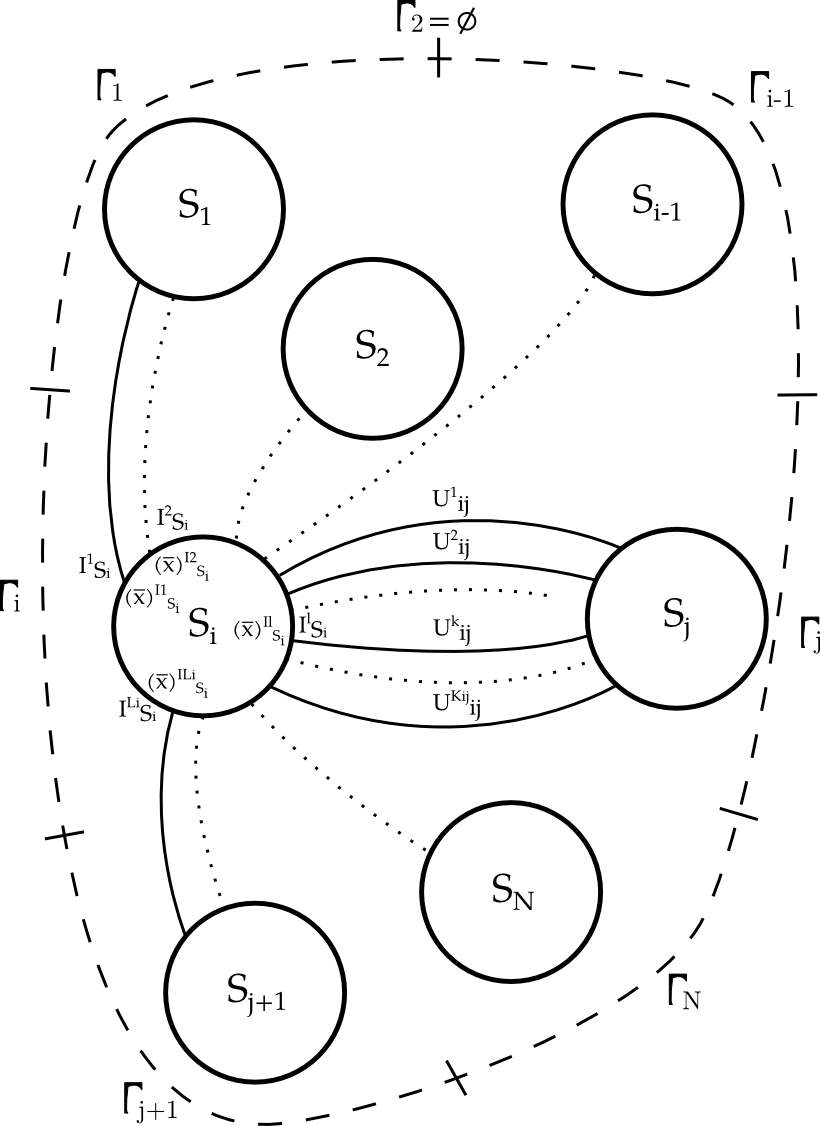
\includegraphics[scale = 0.4]{coupling_systems.png}
\caption[Esquema de descomposición disjunta de dominios]{Esquema de subsistemas de estudio relacionados mediante condiciones de borde dinámicas en interfaces de acoplamiento.} 
\label{esquema-acoplamiento} 
\end{figure}

En principio, existen tantas incógnitas como variables en cada interfaz.
Sin embargo, es posible notar que la unión $U_{i,j}^k$ que relaciona los sistemas $S_{i}$ y $S_{j}$ 
mediante las interfaces $I_{S_{i}}^{l_1}$ e $I_{S_{j}}^{l_2}$ respectivamente, 
define una relación de continuidad\footnote{
Las incógnitas que representan derivadas normales en la interfaz de acople pueden tomar signos opuestos según la convención.
Por ejemplo, si el flujo de calor es una incógnita, 
y se define como flujo positivo a aquel que es saliente del subsistema, 
entonces la condición de continuidad implicará que:
\begin{equation*}
{(q")_{S_i}^{I_{l_1}}}=-{(q")_{S_j}^{I_{l_2}}}
\label{continuidad-q}
\end{equation*}
} entre las incógnitas ${(x_m)_{S_i}^{I_{l_1}}}$ y ${(x_m)_{S_j}^{I_{l_2}}}$, de tal forma que:

\begin{equation}
{(x_m)_{S_i}^{I_{l_1}}}={(x_m)_{S_j}^{I_{l_2}}}
\label{continuidad}
\end{equation}
Estas relaciones reducen a la mitad la cantidad de incógnitas.
Las demás ecuaciones necesarias para despejar las incógnitas se encuentran a partir del modelo de estudio de cada subsistema. 
Sean $(F_m)_{i}^{l}$ las relaciones funcionales que calculan el valor de las incógnitas ${(x_m)_{S_i}^{I_l}}$ en la interfaz $l$ del subsistema $i$,
a partir del valor de otras incógnitas y de los datos de contorno sobre la frontera exterior $\Gamma_i$.
Se tiene que:
\begin{equation}
\begin{split}
  (x_m)_{S_i}^{I_l} = (F_m)_{i}^{l} \left ( (\bar{x})_{S_i}^{I_1}, (\bar{x})_{S_i}^{I_2}, ..., 
  (\bar{x})_{S_i}^{I_{L_i}}, (\alpha_i({\Gamma_i}) \right )
\end{split}
\label{ecuaciones-modelos}
\end{equation}

donde $(\alpha_i({\Gamma_i})$ representa las condiciones de borde impuestas sobre la curva $\Gamma_i$.
Estas relaciones, básicamente, mapean condiciones de borde de un tipo, que son impuestas como datos, en condiciones de borde de otro tipo.
Notar que algunas de las dependencias pueden anularse dependiendo del modelo de estudio utilizado en cada subsistema.
Cuando la expresión \ref{ecuaciones-modelos} es más sencilla y solo involucra el valor de otro tipo de condición de borde en la misma interfaz,
la relación funcional recibe el nombre de operador \textit{Steklov-Poincaré}.
En matemática, el operador \textit{Steklov-Poincaré} mapea el valor de una condición de borde de una PDE elíptica en un dominio al valor
de otra condición de borde (por ejemplo, una condición de borde de tipo \textit{Dirichlet} en una condición de borde de tipo \textit{Neumann}).
Usualmente, cualquiera de las dos condiciones determinan la solución.

\subsection*{Estrategia de resolución}
\label{1:ecuaciones}

A continuación se propone un ejemplo didáctico para comprender las estrategias de acoplamiento posteriormente comentadas. 
Se desea resolver un problema de cálculo de campo de temperatura mediante el Método de Descomposición Disjunta de Dominios.
El sistema global de análisis es una barra unidimensional de longitud $L$ con condiciones de borde homogéneas, fuente interna de energía $f$ y conductividad térmica $k$.
El modelo matemático utilizado es el siguiente:
\begin{equation}
\left\{\begin{matrix}
-k \Delta u=f \\
\left.u\right|_{\partial\Omega}=0
\end{matrix}\right.
\label{ecuacion-calor}
\end{equation}

El dominio original $[0,L]$ es particionado en los subdominios $[0,c]$ y $[c,L]$ (ver Figura \ref{temp-ej}).
Se va a resolver la ecuación \ref{ecuacion-calor} en cada uno de ellos, pero la condición de borde \textit{Dirichlet} ahora solo aplica sobre el borde original del dominio.

\begin{figure}
\centering{}
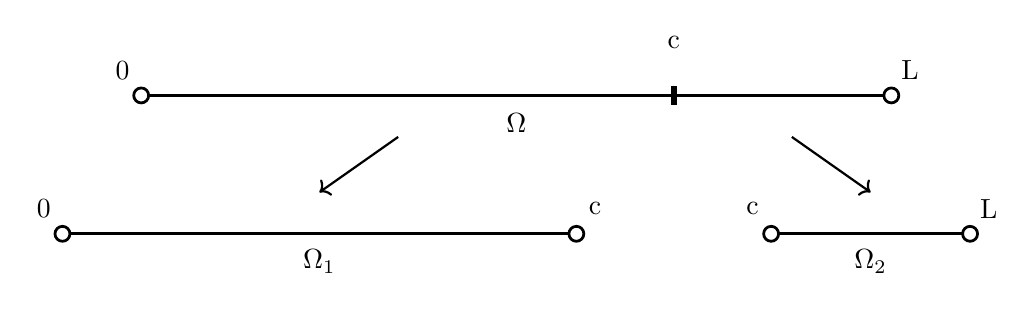
\begin{tikzpicture}
	\node at (12.5,4em) (om) {$\Omega$};

	\node at (7.5,5.9em) (Olabel) {0}; % 0
	\node at (7.5,5em) (O) {}; % point 0

	\node at (14.5,6.9em) (clabel) {c}; % c
	\node at (14.5,5em) (c) {}; % point c

	\node at (17.5,5.9em) (llabel) {L}; % L
	\node at (17.5,5em) (l) {}; % point L

	\draw[line width=1pt, o-|] (O) -- (c.center); % primer extremo de barra completa
	\draw[line width=1pt, |-o] (c.center) -- (l); % segundo extremo de barra completa

	\draw[line width=0.8pt,->] (11,3.5em) -- (10,1.5em); % primer flecha
	\draw[line width=0.8pt,->] (16,3.5em) -- (17,1.5em); % segunda flecha

	\node at (10,-1em) (om1) {$\Omega_1$};
	\node at (6.5,0.9em) (O1label) {0};
	\node at (6.5,0em) (O1) {};
	\node at (13.5,0.9em) (c1label) {c};
	\node at (13.5,0em) (c1) {};

	\draw[line width=1pt, o-o] (O1) -- (c1); % primer barra

	\node at (17,-1em) (om2) {$\Omega_2$};
	\node at (15.5,0.9em) (c2label) {c};
	\node at (15.5,0em) (c2) {};
	\node at (18.5,0.9em) (l2label) {L};
	\node at (18.5,0em) (l2) {};

	\draw[line width=1pt, o-o] (c2) -- (l2); % segunda barra

\end{tikzpicture}
\caption[Descomposición en barra unidimensional]{Descomposición disjunta de dominios en el cálculo del campo de temperatura a lo largo de una barra unidimensional.}
\label{temp-ej}
\end{figure}

Para que cada problema quede bien planteado es necesario imponer una condición de borde extra en el punto de acople $c$ de cada subsistema.
Esta decisión depende del método empleado para resolver el acoplamiento.

La forma clásica de resolución es el método \textit{Dirichlet-to-Neumann}.
Este método es un método explícito de simple implementación, que resuelve el acoplamiento mediante iteraciones de tipo \textit{Piccard}.
En el método \textit{Dirichlet-to-Neumann}, es necesario decidir qué subsistema va a ser resuelto en primera instancia.
Si se decidiera, por ejemplo, comenzar con el subsistema de la izquierda, luego es necesario decidir qué tipo de condición de borde se le va a aplicar.
Estas primeras decisiones son arbitrarias.
Si se decide imponer una temperatura (condición \textit{Dirichlet}) al borde del primer subsistema,
luego de realizar el cálculo de temperaturas quedaría definido un flujo calórico a través de su interfaz de conexión con el segundo subsistema.
Es decir, uno de los valores de las incógnitas en la interfaz de acople se calcula como función del valor de la otra incógnita, 
que fue supuesto como dato, a partir de la relación \ref{ecuaciones-modelos}.
En este caso la relación recibe el nombre de operador \textit{Steklov-Poincaré} y se define como:
\begin{equation}
(q''_{calc})_{S_1} = \mathscr{N}_1\left ((T_{guess})_{S1}\right )
\label{q_n_t}
\end{equation}
donde $\mathscr{L}$ es el operador que mapea condiciones de borde de tipo \textit{Dirichlet} en condiciones de borde de tipo \textit{Neumann},
$(T_{guess})_{S1}$ es la temperatura que fue impuesta como condición de borde en el primer subsistema y $(q''_{calc})_{S_1}$ es el flujo calórico calculado.
En base a la relación de continuidad \ref{continuidad} este flujo de calor se impone en el segundo subsistema como condición de borde.
Esta condición define una temperatura en la interfaz de acople, mediante el segundo operador \textit{Steklov-Poincaré} definido:
\begin{equation}
(T_{calc})_{S_2} = \mathscr{D}_2\left ((q''_{calc})_{S1}\right )
\label{t_d_q}
\end{equation}
donde $\mathscr{D}$ es el operador que mapea condiciones de borde de tipo \textit{Nemaumann} en condiciones de borde de tipo \textit{Dirichlet},
y $(T_{calc})_{S_2}$ es la temperatura calculada.
Si $(T_{calc})_{S_2}$ coincide con $(T_{guess})_{S1}$, los resultados están convergidos y entonces finaliza el cálculo
En caso contrario, el proceso debe repetirse, pero ahora se impone $T_2$ al primer subsistema.
El cálculo continúa así hasta que los valores $\{(q''_{calc})_{S_1}, (T_{calc})_{S_2}\}$ convergen en iteraciones contiguas.
Si inicialmente se hubiera impuesto una condición de tipo \textit{Neumann} en el primer subdominio, 
necesariamente al segundo subdominio debería habérsele impuesto una condición de tipo \textit{Dirichlet},
ya que la variable calculada en la interfaz de acople por el primer subsistema hubiera sido una temperatura.
Es decir, al utilizar el método \textit{Dirichlet-to-Neumann}, la elección de un tipo de frontera en un subdominio dado determina el tipo de frontera en el subdominio contiguo,
para las ecuaciones que relacionan las mismas variables de estado en ambos subsistemas (aquí solo existe una única variable de estado, la temperatura).
Esta característica es un poco restrictiva, ya que no permitiría, por ejemplo, que todos los subproblemas de análisis se resuelvan con condiciones de borde de tipo \textit{Dirichlet}.

Sin embargo esta no es la única desventaja del método \textit{Dirichlet-to-Neumann}.
Otra desventaja es que en general requiere demasiadas iteraciones para converger \cite{fede-enief2016}.
En algunos problemas el método puede quedar estancado, iterando en series de valores que se repiten en ciclo.
Y en otros casos el método es divergente (sin ir más allá, para un cierto conjunto de parámetros del problema ejemplo analizado, el método diverge, ver \cite{coup-strong}).

Existe una forma alternativa de resolver el acoplamiento, y es mediante una técnica implícita.
Esta técnica es una metodología iterativa, y consiste en la evaluación de residuos sucesivos construidos por diferencia entre valores propuestos y valores calculados.
En primera instancia se propone un valor \textit{guess} para todas las incógnitas $(x_{m,guess})_{S_i}^{I_l}$.
Estos valores deben respetar las relaciones de continuidad \ref{continuidad}.
En segunda instancia se decide arbitrariamente qué tipos de condiciones de borde va a recibir cada interfaz de cada subsistema,
definiendo problemas parciales bien planteados.
En el ejemplo analizado, sería posible definir condiciones de borde de tipo \textit{Dirichlet} en ambos subsistemas.
En función de esta decisión, se toman los valores correspondientes del vector $\bar{x}_{guess}$ y se establecen como datos para cada problema parcial.
Una vez resuelto el problema en cada subdominio, se calcula el valor de las variables que no fueron tomadas como dato en las interfaces de acople.
En el ejemplo, si se había establecido un valor de temperatura como condición de borde de tipo \textit{Dirichlet} en ambas interfaces,
se calcula entonces el valor del flujo de calor en la misma interfaz para cada subsistema, mediante los operadores de \textit{Steklov-Poincaré} $\mathscr{N}_1$ y $\mathscr{N}_2$:
\begin{equation}
\left\{\begin{matrix}
(q''_{calc})_{S_1}  = \mathscr{N}_1\left ((T_{guess})_{S1}\right ) \\
(q''_{calc})_{S_2}  = \mathscr{N}_2\left ((T_{guess})_{S2}\right )
\end{matrix}\right.
\label{qq_nn_tt}
\end{equation}

Al hacer esto se están resolviendo las ecuaciones \ref{ecuaciones-modelos},
obteniéndose los valores $(x_{m,calc})_{S_i}^{I_l}$.
Finalmente, se computan las diferencias entre los valores \textit{guess} y los valores calculados, obteniendo los residuos $(r_m)_{i}^{l}$:

\begin{equation}
(r_m)_{i}^{l} = (x_{m,guess})_{S_i}^{I_l} - (x_{m,calc})_{S_i}^{I_l}
\label{ecuaciones-residuos}
\end{equation}
donde $m$ es el índice de incógnita, $l$ de la intefaz e $i$ del subsistema.
En el ejemplo, las ecuaciones de residuos quedarían:
\begin{equation}
\left\{\begin{matrix}
(r_{q''})_{S1}^{1}  = (q''_{guess})_{S_1} - (q''_{calc})_{S_1} \\
(r_{q''})_{S2}^{1}  = (q''_{guess})_{S_2} - (q''_{calc})_{S_2}
\end{matrix}\right.
\label{res_qq}
\end{equation}

La convergencia fuerte de los subsistemas acoplados requiere que estos residuos sean nulos, y por lo tanto se busca el siguiente resultado:
\begin{equation}
\bar{r}=\bar{0}
\label{sistema-simple}
\end{equation}
donde $\bar{r}$ es el vector de residuos de las ecuaciones.
Comúnmente en la primera iteración esto no sucede, y por lo tanto es necesario repetir el proceso sucesivas veces hasta obtener convergencia.
En general los sistemas acoplados se modelan con sistemas de ecuaciones no lineales y por ello se investigan distintos métodos numéricos para la resolución de \ref{sistema-simple}.

\subsection*{Métodos numéricos para la resolución de sistemas de ecuaciones de residuos}
\label{1:metodos}

Existen diferentes métodos numéricos para hallar las raíces del sistema de ecuaciones \ref{sistema-simple}.
Haciendo un desarrollo de Taylor de las ecuaciones de residuos alrededor del punto $\bar{x}_n$, 
truncando los términos superiores al primer orden, y evaluando en $\bar{x}=\bar{x}_{n+1}$ se tiene:

\begin{equation}
\bar{r}(\bar{x}_{n+1}) = \bar{r}(\bar{x}_n) + \nabla \bar{r}(\bar{x}_n)(\bar{x}_{n+1}-\bar{x}_n)
\label{taylor}
\end{equation}
donde $\nabla \bar{r}(\bar{x}_n)$ es la matriz jacobiana del sistema $\mathbb{J}$ evaluada en el punto $\bar{x}_n$, 
cuyo elemento $J_{ij}$ debe evaluarse como $J_{ij}=\frac{\partial r_i}{\partial x_j}$.
Suponiendo que ${\bar{x}_{n+1}}$ tiende a la raíz buscada se ha de cumplir que $\bar{r}(\bar{x}_{n+1})=0$.
Sustituyendo en \ref{taylor} y operando algebraicamente se llega a la siguiente expresión:

\begin{equation}
\bar{r}(\bar{x}_n) = -\mathbb{J}(\bar{x}_n)(\bar{x}_{n+1}-\bar{x}_n)
\end{equation}
Para hallar la solución $\bar{x}_{n+1}$ simplemente hay que resolver el sistema:

\begin{equation}
\bar{x}_{n+1} = \bar{x}_{n} -\mathbb{J}^{-1}(\bar{x}_n)\bar{r}(\bar{x}_n)
\end{equation}
que es el método de iterativo \textit{Newton-Raphson}.
La principal ventaja de este método es que tiene orden de convergencia cuadrática,
pero la desventaja es que para utilizar este método se requiere la construcción de la matriz jacobiana en cada iteración, lo cual es demasiado costoso.
Una sencilla aproximación mediante diferencias finitas de primer orden de cada elemento de la matriz jacobiana requiere numerosas evaluaciones.
Cada elemento $J_{ij}=\frac{\partial R_i}{\partial x_j}$ puede aproximarse mediante diferencias finitas a primer orden como:
\begin{equation}
J_{ij} \approx \frac{r_i(\bar{x}_j + \Delta \bar{x}_j) - r_i(\bar{x}_j)}{\left\|\Delta x_j\right\|}
\label{j-diff}
\end{equation}
donde $\Delta \bar{x}_j$ es un vector que contiene valores nulos en todos sus elementos excepto en el elemento de la posición $j$,
cuyo valor es la diferencia incremental para esa variable $j$.
La construcción de la matriz jacobiana con éste método requiere una evaluación del vector residuo $\bar{r}$ en el punto $\bar{x}$ y luego $N_{unk}$ evaluaciones extras,
donde $N_{unk}$ es la cantidad total  de incógnitas. 
Es decir, en total, se requieren $N_{unk}+1$ evaluaciones.
Si bien estas evaluaciones son independientes entre sí y por lo tanto altamente paralelizables, este método requeriría excesivos recursos de cálculo.

Una forma alternativa y elegante de resolver el sistema de ecuaciones planteado en \ref{sistema-simple} es mediante métodos \textit{quasi-Newton}.
La característica principal de estos métodos es que aproximan la matriz jacobiana sin necesidad de realizar evaluaciones extras, y por lo tanto tienen una ventaja fuerte frente al método de \textit{Newton-Raphson}.
Además, tienen convergencia superlineal \cite{broyden-on}, y por lo tanto también presentan una ventaja frente a los métodos mediante iteraciones de \textit{Piccard}. 

El método de \textit{Broyden} es uno de estos métodos \cite{broyden}.
La matriz jacobiana $\mathbb{B}_n$ en la iteración $n$ es aproximada mediante una matriz $\mathbb{B}_n$ que se construye solo en función 
del valor de los vectores incógnitas $\bar{x}_{n-1}$ y $\bar{x}_{n}$,
de los vectores residuos $\bar{r}_{n-1}$ y $\bar{r}_{n}$,
y de la matriz de la iteración previa $\mathbb{B}_{n-1}$:
\begin{equation}
\mathbb{B}_n = \mathbb{B}_{n-1} + \frac{\Delta{\bar{r}_n}-\mathbb{B}_{n-1}\Delta{\bar{x}_n}}{\left \| \Delta{\bar{x}_n} \right \| ^2}\Delta{\bar{x}}_n^T
\label{broyden}
\end{equation}
donde $\Delta{\bar{r}_n}=\bar{r}_n - \bar{r}_{n-1}$ y $\Delta{\bar{x}_n}=x_n - \bar{x}_{n-1}$.
Existe una variante del método, el método \textit{Broyden ortonormal}, que aproxima la matriz $\mathbb{B}_n$ en función de una base vectorial de residuos previos calculados.
Este método asegura la convergencia en una cantidad finita de iteraciones para sistemas lineales \cite{broyden-on}, (la cantidad de iteraciones requerida es la dimensión de la matriz jacobiana).

Existe también un conjunto de métodos conocidos como métodos \textit{Newton-Krylov} para la resolución del sistema \ref{sistema-simple}. Estos métodos no requieren el cálculo de matriz jacobiana ya que resuelven el sistema mediante técnicas de gradientes descendentes. Sin embargo, en cada paso de descenso requieren evaluaciones de residuos, y por tanto son altamente costosos.

Notar que los métodos presentados en el presente apartado resuelven el sistema de ecuaciones \ref{sistema-simple} de forma monolítica,
y es por este motivo que permiten incluir estrategias para la selección de condiciones de borde prohibidas al método \textit{Dirichlet-to-Neumann}.
Podría pensarse que el método \textit{Dirichlet-to-Neumann} resuelve un sistema de ecuaciones similar pero solo para ciertas estrategias de condiciones de borde y en forma segregada,
actualizando los valores de las variables a medida que avanza en el cálculo.
En este caso, los residuos se definirían como la diferencia entre el valor de las variables calculadas en dos iteraciones consecutivas.
Para el ejemplo de cálculo de temperaturas analizado en este capítulo, si se comenzara resolviendo el subsistema izquiero, en la iteración $n$ el sistema de ecuaciones a resolver quedaría:
\begin{equation}
\left\{ \begin{array}{rcccl}
(r_{q''})_{S1}^{1} &=& (q''_{calc,n})_{S_1} - (q''_{calc,n-1})_{S_1} &=&\mathscr{N}\left(\left(T_{calc,n-1}\right )_{S_2}\right) - (q''_{calc,n-1})_{S_1} \\
(r_{T})_{S2}^{1} &=& (T_{calc,n})_{S_2} - (T_{calc,n-1})_{S_2} &=& \mathscr{D}\left(\left(q''_{calc,n}\right )_{S_1} \right ) - (T_{calc,n-1})_{S_2}
\end{array}\right.
\label{res_qt}
\end{equation}
donde se ha supuesto que $\left(T_{guess,n}\right )_{S_1}=\left(T_{calc,n-1}\right )_{S_2}$,
y que $\left(q''_{guess,n}\right )_{S_2}=\left(q''_{calc,n}\right )_{S_1}$,
empleando las relaciones de continuidad \ref{continuidad}.

\subsection*{Problemas de evolución}
\label{1:evolucion}
En problemas de evolución la estretegia es permitir que cada subsistema avance por separado acoplando sus resultados mediante las ecuaciones \ref{sistema-simple} solo cada ciertos pasos.
Esto se permite porque cada subsistema podría requerir subpasos de evolución diferentes\footnote{
Distintos subdominios pueden tener diferentes requisitos sobre el parámetro de evolución, dependiendo de la física implicada.
Algunos, por ejemplo, podrían experimentar transitorios fluidodinámicos, en los que es de interés mantener por debajo de algún valor 
ciertos parámetros numéricos (como el número de \textit{Courant}) proporcionales al paso de tiempo.
Otros, en cambio, podrían estar siendo resueltos mediante métodos complejos que consumieran elevados recursos temporales,
por tanto sería de interés utilizar subpasos evolutivos mayores.
}. Notar que no es necesario mantener la misma estrategia de selección de condiciones de borde para cada interfaz a lo largo de la evolución.
Las variables que son datos o incógnitas para cada subdominio pueden irse alternando,
seleccionando diferentes ecuaciones \ref{ecuaciones-modelos} a resolver en diferentes pasos de acople.
Debido a la convergencia fuerte de los valores de las variables en las interfaces de acople,
el método es incondicionalmente estable a lo largo de la evolución.

\section{Objetivos y estructura de trabajo}
\label{1:objetivos}
Considerando la motivación y la formulación precedente, queda establecido el siguiente objetivo general de la maestría:

\vspace{1em}
\begin{addmargin}[1.5em]{1.5em}
\textit{Implementar el acoplamiento fuerte entre modelos dimensionalmente heterogéneos,
resolviendo cada subdominio por separado con códigos particulares, e imponiendo la
interacción entre ellos sólo mediante condiciones de borde.}
\end{addmargin}
\vspace{1em}

La estructura de la tesis es detallada a continuación.
En el presente \hyperlink{chapter.1}{capítulo} se han planteado las ecuaciones que surgen al dividir sistemas complejos mediante interfaces con condiciones de borde dinámicas,
y se han presentado alternativas numéricas para la resolución de las mismas.
En el \hyperlink{chapter.2}{Capítulo 2} se describe la estrategia para la resolución de problemas acoplados mediante diferentes programas de cálculo.
Se presenta la estructura de comunicación definida y se describen las implementaciones necesarias para su funcionamiento.
En el \hyperlink{chapter.3}{Capítulo 3} se muestran algunas aplicaciones de la herramienta estudiada.
La primera aplicación es un sistema fluídico cerrado gobernado por fuerzas naturales, que se estudia subdividiéndolo en dos subsistemas, con dos interfaces de acople cada uno.
El siguiente sistema de estudio es el vaciado del tanque reflector de un reactor de investigación.
Interesa analizar el tiempo de descarga ya que el mismo es diseñado como Segundo Sistema de Parada (SSP).
Se abordan distintos modelos multiescala del mismo, para estudiar el detalle fluídico tridimensional en un componente del sistema,
acoplando con condiciones de borde dinámicas a modelos cero-dimensionales que representan el resto del sistema.
El tercer sistema de análisis es un modelo de redes hidráulicas con múltiples componentes.
Con este estudio se busca demostrar la eficiencia de la herramienta en acoples fluidodinámicos de mayor escala.
Sobre el final del capítulo se extiende la herramienta a problemas multifísicos.
Se analiza un ejemplo de aplicación al problema neutrónico-termohidráulico.

 % intro
\chapter{Estrategia de acoplamiento}
\label{chap2}
\chapterquote
%~ {We build too many walls and not enough bridges.}
{Construimos demasiadas murallas y no suficientes puentes.}
{Sir Isaac Newton, 1643-1727}

\section{Paradigma maestro-esclavo}
\label{2:maestro-esclavo}
La estrategia general para la resolución de problemas acoplados mediante el método de descomposición disjunta de dominios es comentada a continuación.
Los problemas parciales pertenecientes a distintos subdominios se resuelven con diferentes códigos específicos.
Cada uno de estos códigos recibe valores de condiciones de borde y en base a ellos se encarga de calcular el valor de las incógnitas en las interfaces de acople mediante las ecuaciones \ref{ecuaciones-modelos}.
Existe un único programa que acopla los resultados.
Este programa se abstrae completamente de la física implicada en cada subsistema.
Simplemente recibe los valores para las incógnitas calculados por los diferentes programas y con ellos resuelve el sistema de ecuaciones de residuos \ref{ecuaciones-residuos}.
En base a estos residuos propone\footnote{
Esta propuesta reside en el método de resolución de ecuaciones no lineales seleccionado, ver sección \ref{1:metodos}.
} nuevos valores para las inćognitas en las interfaces de acople y los comunica nuevamente a los demás programas.
Este tipo de comunicación utilizado recibe el nombre de \textit{maestro-esclavo} \cite{maestro-esclavo},
en el cual existe un programa \textit{maestro} que tiene el control unidireccional sobre los demás programas, que actúan bajo el rol de \textit{esclavos}.
Además del envío y recepción de valores de variables, son funciones del código \textit{maestro} el envío de órdenes a sus \textit{esclavos} de comenzar el cálculo en un dado paso de evolución, reiniciar el cálculo o incluso abortar.

Cabe notar que cada código \textit{esclavo} podría ejecutarse en varios procesos, paralelizando sus cálculos,
ya sea mediante memoria compartida como mediante memoria distribuida.
Incluso podrían lanzarse diferentes procesos del código \textit{maestro} en la resolución de algún problema.
Debido a la complejidad en destinatarios de mensajes, cantidades y tipos de variables a compartir,
es necesario definir una estrategia clara de comunicación
que permita acoplar diversos códigos de manera genérica, segura y eficaz.
La estrategia definida es comentada en la siguiente sección.

\section{Modelos de comunicación}
\label{2:comunicacion}

La configuración \textit{maestro-esclavo} requiere la ejecución de múltiples programas independientes.
Al mismo tiempo, cada código podría estar corriendo en forma paralelizada\footnote{
En general, cada programa \textit{esclavo} es un programa que ya ha sido utilizado y validado para algún tipo de cálculo.
Si el código está paralelizado, en base a estudios de \textit{speedup} se podría tener cierta experiencia en su modo de ejecución óptimo para alguna tarea dada.
Esta ejecución podría requerir múltiples nodos en un clúster, por ejemplo.
}.
Debido a esta complejidad es necesario planificar la estrategia de comunicación considerando la distribución del cálculo en múltiples procesadores,
con el objetivo de no perder generalidad en la herramienta desarrollada.
Los modos de comunicación implementados son los siguientes:
\begin{itemize}
\item Paso de mensajes: este modo es implementado para comunicar procesos de programas en los cuales es posible modificar los códigos fuente.
\item Lectura y escritura de archivos de entrada y salida: este modo es implementado para comunicar procesos de programas en los cuales no es posible modificar los códigos fuente.
\end{itemize}

En ambos casos los programas esclavos se comunican solo con el programa maestro.
Si bien estos tipo de comunicaciones remotas son más lentas que las
comunicaciones locales, en general su latencia es despreciable frente al tiempo de cálculo de los procesos \textit{esclavos}.

\subsection*{Paso de mensajes}
\label{2:mpi}

En sistemas de memoria distribuida, el paso de mensajes es un método de
programación utilizado para realizar el intercambio de datos entre
procesos \cite{comunicacion}. 
El paso de mensajes involucra la transferencia de datos desde un proceso
que envía a otro proceso que recibe. 
El proceso que envía,
necesita conocer la localización, el tamaño y el tipo de los datos, así como el
proceso destino.

Estas funcionalidades se implementaron siguiendo el protocolo del estándard Interfaz de Paso de Mensajes (MPI por sus siglas en inglés, \textit{Message Passing Interface}). 
MPI es una especificación de paso de mensajes aceptada como estándar
por todos los fabricantes de computadores. 
El objetivo principal de MPI es proporcionar un estándar para escribir
programas (lenguajes \texttt{C}, \texttt{C++}, \textit{texttt}) con paso de mensajes. De esta forma, se
pretende mejorar la portabilidad, el rendimiento, la funcionalidad y
la disponibilidad de las aplicaciones.

Se utilizaron dos implementaciones alternativas.
En la primera, cada código \textit{esclavo}, así como el código \textit{maestro},
es ejecutado de manera independiente en uno (SISD por sus siglas en inglés, Single Instruction, Single Data) o múltiples procesos (SIMD por sus siglas en inglés, Single Instruction, Multiple Data).
El código \textit{maestro} publica una serie de puertos a los cuales cada código \textit{esclavo} puede conectarse\footnote{
Para que los programas puedan encontrar los puertos publicados, es necesario que todos ellos pertenezcan a un mismo servicio de comunicación generado por el \textit{ompi-server}.
}.
Una vez aceptadas las conexiones, los programas pueden intercambiar mensajes con él siguiendo una lógica preestablecida.
Cuando ya no es necesario que los programas continúen comunicándose, se cierran las conexiones.

En la otra implementación, todos los programas son ejecutados al mismo tiempo en uno (MISD por sus siglas en inglés, Multiple Instruction, Single Data) o varios procesos (MIMD por sus siglas en inglés, Multiple Instruction, Multiple Data).
En este tipo de ejecuciones todos los procesos cuentan con un único comunicador original, \textit{MPI\_COMM\_WORLD}, y por ello es necesario crear nuevos grupos de procesos y de comunicadores.
Una vez establecidos los comunicadores, los programas ya pueden intercambiar mensajes con el código \textit{maestro} siguiendo la misma lógica que se establecerá para ambos modelos.
Si bien esta implementación no es posible para nuevas conexiones una vez que los programas han sido ejecutados,
son mucho más seguras, ya que no dependen del éxito de encontrar los puertos requeridos para las conexiones.

\subsection*{Lectura y escritura de archivos de entrada y salida}
\label{2:io}

La comunicación mediante lectura y escritura de archivos se implementó para demostrar la capacidad de acoplar códigos cuyos códigos fuente no son capaces de ser modificados.
La idea principal es ejecutar corridas simples del código \textit{esclavo} administradas desde el código \textit{maestro}.
Para ello el código \textit{maestro} escribe en el archivo de entrada del programa \textit{esclavo} todos los parámetros necesarios para la ejecución del cálculo,
ordena su ejecución, espera a que este termine y luego realiza una búsqueda de los valores de las variables de interés en archivos de salida.
En problemas de evolución, el código \textit{maestro} debe notificar en el archivo de entrada el parámetro de evolución,
así como otros valores de variables de estado del paso previo,
ya que cada corrida del código \textit{esclavo} solo vive para realizar un cálculo entre dos pasos de evolución acoplados.

La ejecución de programas \textit{esclavos} se implementó de dos formas alternativas.
La primera forma es mediante el uso de la función \textit{system} de la librería de \textit{c}.
Esta función deja al proceso que la ejecuta en pausa hasta que el programa \textit{esclavo} finaliza, cuando ella retorna algún mensaje de error o de éxito.
La ventaja de esto es que no debe implementarse alguna función extra para conocer cuándo leer los archivos de salida del programa \textit{esclavo}.
Sin embargo, no es posible disparar múltiples procesos de un programa mediante la función \textit{system} desde un proceso que actualemente utiliza \textit{MPI}.
Ésta prohibición es necesaria para controlar el disparo de procesos.
Para este tipo de ejecuciones, existe la función \textit{MPI\_Comm\_Spawn} de \textit{MPI}, que se implementó como forma alternativa de ejecución de programas \textit{esclavos}.
Esta función permite especificar la cantidad de procesos de ejecución del programa a disparar.
El problema es que la función devuelve el control al programa \textit{maestro} de forma instantánea, sin esperar a que el código disparado finalice,
por lo que, en principio, debe implementarse alguna función extra para saber cuándo es posible leer el archivo de salida.

Es necesario notar que este modelo de comunicación no es tan eficiente como el de intercambio de mensajes,
ya que la lectura y escritura de archivos consume mayores recursos de tiempo, por lo que, siempre que fuera posible, es recomendable implementar el otro modelo.
Además, requiere la programación de rutinas extras específicas dedicadas a la escritura de archivos de entrada y lectura de archivos de salida de distintos códigos \textit{esclavos}.

\subsection*{Estructura de comunicación implementada}
\label{2:estructura}

Se desarrollaron funciones híbridas con la finalidad de cubrir todas las formas de comunicación descriptas en la sección previa.
En el caso de comunicación por intercambio de mensajes, 
la estrategia definida establece comunicaciones siempre entre un único proceso del código \textit{maestro}, el proceso \textit{raíz},
y un único proceso de cada código \textit{esclavo} (sus propios procesos \textit{raíces}\footnote{
Es responsabilidad del código \textit{esclavo} la comunicación de los datos recibidos por el proceso \textit{raíz} a los demás procesos.
}).
En el caso de lectura y escritura de archivos y ejecución de programas \textit{esclavos},
la estrategia definida paraleliza las responsabilidades entre todos los procesos lanzados del código \textit{maestro}.
El esquema \ref{esquema-comunicacion} resume la estrategia de comunicación.

\begin{figure}
\centering{}
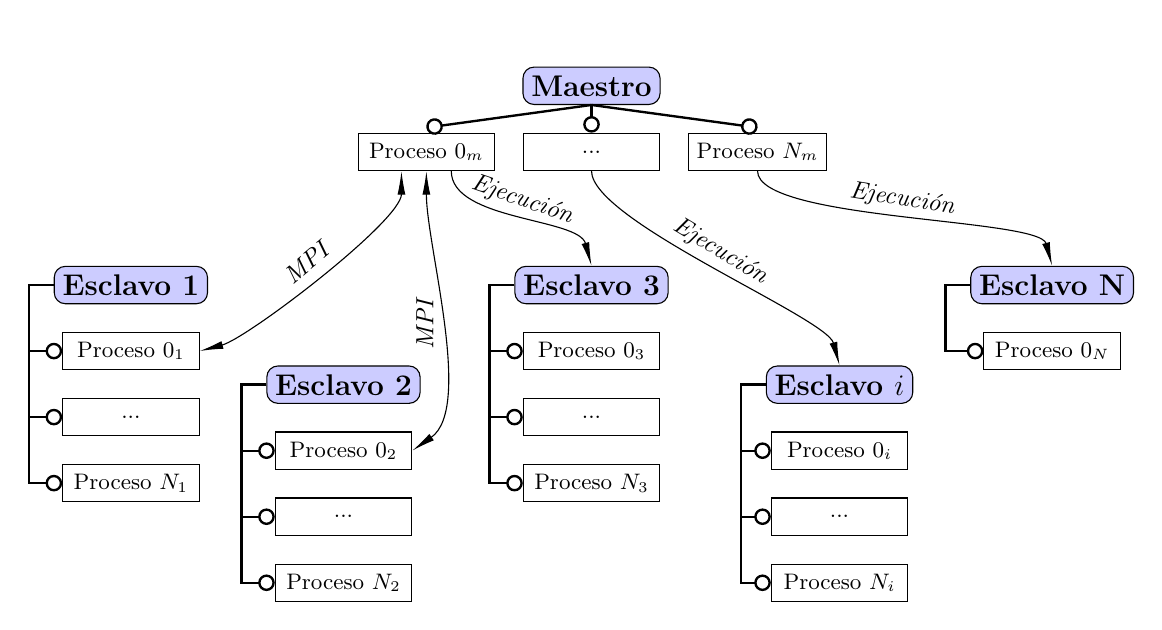
\begin{tikzpicture}[
  scale=0.9, every node/.style={scale=0.9},
	block1/.style={
	draw,
	fill=white,
	rectangle, 
	minimum width={width("Proceso $N_m$")+2pt},
	minimum height={15pt},
	font=\small},
	block2/.style={
	draw,
	fill=white,
	rectangle,
  fill=blue!20,
  text centered, 
  rounded corners,
	minimum width={width("Esclavo N")+2pt},
	minimum height={15pt},
	font=\large},
	connector/.style={
	-o,
	line width=0.3mm
	},
  arrow1/.style={
  -{Latex[length=3mm, width=1mm]}
  },
  arrow2/.style={
  {Latex[length=3mm, width=1mm]}-{Latex[length=3mm, width=1mm]}
  }]

	% Dummy
	\node at (0,10em)             (dummy) {}; % blank space

	% Master
	\node [block2] at (0,8em)             (master) {\textbf{Maestro}};
	\node [block1, below=1em of master]   (masterp1) {...};
	\node [block1, left=1em of masterp1]  (masterp0) {Proceso $0_m$};	
	\node [block1, right=1em of masterp1] (masterpN) {Proceso $N_m$};

	% Slave 1
	\node [block2] at (-6.5,0em)    		(slave1) {\textbf{Esclavo 1}};
	\node [block1, below=1em of slave1] (s1p0) 	 {Proceso $0_1$};
	\node [block1, below=1em of s1p0]   (s1p1) 	 {...};
	\node [block1, below=1em of s1p1] 	(s1pN) 	 {Proceso $N_1$};
	
	% Slave 2
	\node [block2] at (-3.5,-4em)    		(slave2) {\textbf{Esclavo 2}};
	\node [block1, below=1em of slave2] (s2p0) 	 {Proceso $0_2$};
	\node [block1, below=1em of s2p0]   (s2p1) 	 {...};
	\node [block1, below=1em of s2p1] 	(s2pN) 	 {Proceso $N_2$};
	
	% Slave 3
	\node [block2] at (0,0em)      		  (slave3) {\textbf{Esclavo 3}};
	\node [block1, below=1em of slave3] (s3p0) 	 {Proceso $0_3$};
	\node [block1, below=1em of s3p0]   (s3p1) 	 {...};
	\node [block1, below=1em of s3p1] 	(s3pN) 	 {Proceso $N_3$};
	
	% Slave 4
	\node [block2] at (3.5,-4em)   		  (slave4) {\textbf{Esclavo $i$}};
	\node [block1, below=1em of slave4] (s4p0) 	 {Proceso $0_i$};
	\node [block1, below=1em of s4p0]   (s4p1) 	 {...};
	\node [block1, below=1em of s4p1] 	(s4pN) 	 {Proceso $N_i$};
	
	% Slave N
	\node [block2] at (6.5,0em)    		  (slave5) {\textbf{Esclavo N}};
	\node [block1, below=1em of slave5] (s5p0) 	 {Proceso $0_N$};

	% Processes
	\draw[connector] (master.south) -- ($(masterp0.north)+(0,0.2em)$);
	\draw[connector] (master.south) -- ($(masterp1.north)+(0,0em)$);
	\draw[connector] (master.south) -- ($(masterpN.north)+(0,0.2em)$);

	\draw[connector] (slave1.west) -- ++(-1em,0) |- (s1p0.west);
	\draw[connector] (slave1.west) -- ++(-1em,0) |- (s1p1.west);
	\draw[connector] (slave1.west) -- ++(-1em,0) |- (s1pN.west);

	\draw[connector] (slave2.west) -- ++(-1em,0) |- (s2p0.west);
	\draw[connector] (slave2.west) -- ++(-1em,0) |- (s2p1.west);
	\draw[connector] (slave2.west) -- ++(-1em,0) |- (s2pN.west);

	\draw[connector] (slave3.west) -- ++(-1em,0) |- (s3p0.west);
	\draw[connector] (slave3.west) -- ++(-1em,0) |- (s3p1.west);
	\draw[connector] (slave3.west) -- ++(-1em,0) |- (s3pN.west);

	\draw[connector] (slave4.west) -- ++(-1em,0) |- (s4p0.west);
	\draw[connector] (slave4.west) -- ++(-1em,0) |- (s4p1.west);
	\draw[connector] (slave4.west) -- ++(-1em,0) |- (s4pN.west);

	\draw[connector] (slave5.west) -- ++(-1em,0) |- (s5p0.west);


	% Comunicators
	\draw[arrow2] ($(masterp0.south)-(1em,0)$) to[out=-90, in=15, distance=2em] node [midway, sloped, anchor=center, above]{\textit{MPI}} (s1p0.east);

	\draw[arrow2] ($(masterp0.south)+(0em,0)$) to[out=-90, in=35, distance=3em] node [midway, rotate=90, anchor=center, above]{\textit{MPI}} (s2p0.east);

	\draw[arrow1] ($(masterp0.south)+(1em,0)$) to[out=-90, in=105, distance=2em] node [midway, sloped, anchor=center, above]{\textit{Ejecución}} (slave3.north);

	\draw[arrow1] (masterp1.south) to[out=-90, in=105, distance=2em] node [midway, sloped, anchor=center, above]{\textit{Ejecución}} (slave4.north);

	\draw[arrow1] (masterpN.south) to[out=-90, in=105, distance=2em] node [midway, sloped, anchor=center, above]{\textit{Ejecución}} (slave5.north);

\end{tikzpicture}
\caption[Esquema de comunicación implementado]{Esquema de comunicación entre los programas \textit{esclavos} y el programa \textit{maestro} implementado en el acoplamiento de códigos.
Los \textit{esclavos} se comunican solo con el \textit{maestro} y no intercambian datos entre sí.
Se utilizan dos modelos de comunicación diferentes.
En el primero, cada código \textit{esclavo} es comunicado con el código \textit{maestro} a través de intercambio de mensajes por \textit{MPI}.
Como podrían correr en modo serial o paralelo, solo sus procesos \textit{raíces} establecen la comunicación con el proceso \textit{raíz} del programa \textit{maestro}.
En el segundo modelo de comunicación, los códigos \textit{esclavos} son directamente \textit{ejecutados} por el programa \textit{maestro} en uno o varios procesos.
En este modelo, la comunicación se establece solo mediante lectura y escritura de archivos.}
\label{esquema-comunicacion}
\end{figure}

\section{Códigos maestros utilizados}
\label{2:maestros}

En este trabajo se utilizaron dos códigos maestros que cumplen con la estrategia de acoplamiento descripta previamente.
El primer código \textit{maestro} utilizado es el código \textbf{Coupling} \cite{coup-0d3d} \cite{coup-black} \cite{coup-hyd}.
\textbf{Coupling} utiliza los modelos de comunicación por paso de mensaje entre programas ejecutados en modos SISD y SIMD.
El código maestro está diseñado de tal forma que los códigos acoplados resuelvan las ecuaciones \ref{ecuaciones-modelos}
para incógnitas en interfaces con condiciones de borde de tipo \textit{Dirichlet} o de tipo \textit{Neumann}.
Con la idea de extender estas capacidades al acoplamiento de programas en modos MISD y MIMD,
al acoplamiento de programas por lectura y escritura de archivos,
así como a programas cuyos cálculos no dependieran exclusivamente de variables seteadas como condiciones de borde,
sino de otros parámetros generales del sistema,
se desarrolló un código más genérico de acoplamiento, el código \textbf{Newton} \cite{newton}.
En los Apéndices \ref{C:coupling} y \ref{C:newton} se describen las principales características de ambos códigos.

\section{Arquitectura de acoplamiento montada en códigos \textit{esclavos} comunicados por paso de mensajes}
\label{2:arquitectura-mpi}

En general, los códigos \textit{esclavos} son programas de cálculo particulares que no han sido diseñados para mantenerse acoplados a otros códigos.
En esta sección se demuestra cómo mediante unas mínimas modificaciones en sus rutinas es posible implementar un acoplamiento eficiente por paso de mensajes.

Las acciones de acoplamiento se reúnen en cuatro instancias diferentes:
\begin{enumerate}
\item al principio del programa;
\item al principio de cada paso de evolución acoplado;
\item al finalizar cada paso de evolución acoplado;
\item al finalizar el programa.
\end{enumerate}
En cada una de estas instancias el programa \textit{esclavo} debe llamar a una función específica de acoplamiento.
El programador podría definir una nueva variable \textit{booleana} que a modo de bandera indique cuándo se está realizando un cálculo acoplado para realizar el llamado o evadirlo.
Los problemas que no involucran evolución de variables pueden ser tratados como problemas con un solo paso de evolución.
A continuación se describen las instancias de acoplamiento.

\subsection*{Acoplamiento en instancia 1: al principio del programa}

En esta instancia es necesario establecer la comunicación \textit{MPI} entre el proceso \textit{raíz} del código \textit{esclavo} y el código maestro.
Si ambos programas han sido ejecutados en los esquemas SISD o SIMD los pasos a realizar son los siguientes:
\begin{itemize}
\item búsqueda del puerto publicado por el el proceso \textit{raíz} del programa \textit{maestro};
\item conexión del proceso \textit{raíz} del programa esclavo a este puerto y creación del comunicador.
\end{itemize}
Si, en cambio, los programas han sido ejecutados en los modos MISD o MIMD, los pasos a realizar son los siguientes:
\begin{itemize}
\item creación de grupo global de procesos;
\item creación de subgrupo local de procesos;
\item creación de un comunicador dentro del subgrupo previo, necesario para el paso de mensajes dentro del programa;
\item creación de un grupo entre el proceso \textit{raíz} del programa esclavo y el proceso \textit{raíz} del programa \textit{maestro};
\item creación de un comunicador en el grupo previo, necesario para el paso de mensajes de acople.
\end{itemize}
Una vez implementada la comunicación, el código \textit{esclavo} puede recibir datos generales 
(como parámetros de evolución iniciales, cantidad de pasos de evolución, cantidad de incógnitas en interfaces de acople, cantidad de interfaces de acople, etc.),
y chequear la consistencia con los datos propios del programa.
Si es necesario, los datos locales pueden ser cambiados notificando al usuario.

\subsection*{Acoplamiento en instancia 2: al principio de cada paso de evolución acoplado}

La estrategia de acoplamiento se define entre el parámetro de evolución inicial $t_{coup,0}$ y el parámetro final $t_{coup,N}$,
con $N+1$ pasos de acoplamiento cada $\Delta t_{coup}=\frac{t_{coup,N} - t_{coup,0}}{N}$.
La solución para $t_{coup,0}$ es la condición inicial del problema, y es dato para todos los programas.
En este paso se llama a la instancia 2, en la cual se recibe valores de condiciones de borde para el primer paso de acoplamiento, en $t_{coup,1}$.
En base a estos valores, el programa \textit{esclavo} resuelve las ecuaciones implicadas en el subdominio correspondiente.
Es posible que además utilice subpasos de evolución $\Delta t_{local}$ locales (como se explicó en el apartado \ref{1:evolucion}  \textbf{Problemas de evolución}),
por lo cual requerirá valores extras para las condiciones de borde en estos pasos. 
En estos casos, se implementa una estrategia de interpolación de valores entre la solución acoplada previa, y los valores recibidos para el siguiente paso acoplado.
Este proceso se repite al principio de cada paso de acople.

\subsection*{Acoplamiento en instancia 3: al finalizar cada paso de evolución acoplado}

Una vez resuelto cada $\Delta t_{coup}$, el programa \textit{esclavo} envía al programa \textit{maestro} los valores de las incógnitas calculadas en las interfaces de acoplamiento.
Tras este envío, el programa queda en espera de la órden para continuar.
Mientras, el programa \textit{maestro} recepciona los valores de las incógnitas calculados por los demás códigos \textit{esclavos}.
Con estos valores resuelve las ecuaciones de residuos \ref{sistema-simple}.
Si el módulo del residuo cae por debajo de cierta tolerancia prefijada el código \textit{maestro} acepta los resultados y envía a sus \textit{esclavos} la órden de continuar con el cálculo.
En caso contrario, puede enviarles la órden de volver a calcular el mismo paso de acoplamiento, o incluso de abortar el cálculo.


\pgfdeclarelayer{bg}    % declare background layer
\pgfsetlayers{bg,main}  % set the order of the layers (main is the standard laye

\begin{figure}
\centering{}
\begin{tikzpicture}[
	block1/.style={
	draw,
	fill=white,
  text centered,
	rectangle, 
	minimum width={width("Proceso $N_m$")+2pt},
	minimum height={17pt},
	font=\small},
	block2/.style={
	draw,
	rectangle,
  fill=blue!20,
  text centered, 
  rounded corners,
	minimum width={width("Esclavo N")+2pt},
	minimum height={15pt},
	font=\large},
	connector/.style={
	-o,
	line width=0.3mm
	},
  arrow1/.style={
  -{Latex[length=3mm, width=1mm]}
  },
  arrow2/.style={
  {Latex[length=3mm, width=1mm]}-{Latex[length=3mm, width=1mm]}
  }
  ]

	% Dummy
	\node at (0,10em)             (dummy) {}; % blank space

	% Códigos
	\node [block2] at (0,20em)          (maestro)   {\textbf{Maestro}};
	\node [block2, left=4.8em  of maestro] (esclavo1) {\textbf{Esclavo $1$}};	
	\node [block2, right=4.8em of maestro] (esclavo2) {\textbf{Esclavo $2$}};
  
  % guess0
  \node [block1, text width=2cm] at (0,16em) (guess0) {cálculo de \scriptsize \{$x_{guess}(t_{coup,1})$, $y_{guess}(t_{coup,1})$\}};
  
  % ci
  \node [anchor=east, text width=2cm, text centered] at (-7 em,18em) (ci1) {\scriptsize (condiciones iniciales)};
  \node [anchor=west, text width=2cm, text centered] at ( 7 em,18em) (ci2) {\scriptsize (condiciones iniciales)};
 
  % s1
  \node [anchor=east] at (-11.5 em,17em) (tl10) {\footnotesize $t_{e1,0}$};  
  \node at (-7.3em,17em) (dummy11) {};
  \draw [dashed] ($(tl10)+(1em,-0.3em)$) -- ($(dummy11)-(0,0.3em)$);
  
  \node [anchor=east] at (-11.5 em,15em) (tl11) {\footnotesize $t_{e1,1}$};  
  \node at (-7.3em,15em) (dummy21) {};
  \draw [dashed] ($(tl11)+(1em,-0.3em)$) -- ($(dummy21)-(0,0.3em)$);
  
  \node [anchor=east] at (-11.5 em,13em) (tl12) {\footnotesize $t_{e1,2}$};  
  \node at (-7.3em,13em) (dummy31) {};
  \draw [dashed] ($(tl12)+(1em,-0.3em)$) -- ($(dummy31)-(0,0.3em)$);
  
  \node [anchor=east] at (-11.5 em,11em) (tl1i) {\footnotesize $t_{e1,i}$};  
  \node at (-7.3em,11em) (dummy41) {};
  \draw [dashed] ($(tl1i)+(1em,-0.3em)$) -- ($(dummy41)-(0,0.3em)$);
  
  \node [anchor=east] at (-11.5 em,9em) (tl1n) {\footnotesize $t_{e1,N}$};  
  \node at (-7.3em,9em) (dummy51) {};
  \draw [dashed] ($(tl1n)+(1.2em,-0.3em)$) -- ($(dummy51)+(0.2em,-0.3em)$);
   
  % Delta t coup 1
  \node [anchor=east] at (-15.25em,17em) (tc0)  {\footnotesize $t_{coup,0}$};
  \node [anchor=east] at (-15.25em,9em) (tc1)  {\footnotesize $t_{coup,1}$};
  \node at(-17.5em,13em) (dtc1) {$\Delta t_{coup}$};
  \draw[|-] ($(tc0.south)+(-1.75em,1em)$) to[out=-90, in=90] ($(dtc1.north)-(1em,0)$);
  \draw[-|] ($(dtc1.south)-(1em,0)$) to[out=-90, in=90] ($(tc1.north)+(-1.75em,-1em)$);
  
  % flechas s1
  \draw[->] ($(tl10.east)+(1.8em,-0.7em)$) -- ($(tl10.east)+(1.8em,-2em)$);
  \draw[->] ($(tl11.east)+(1.8em,-0.7em)$) -- ($(tl11.east)+(1.8em,-2em)$);
  \draw[->] ($(tl12.east)+(1.8em,-0.7em)$) -- ($(tl12.east)+(1.8em,-2em)$);
  \draw[->] ($(tl1i.east)+(1.8em,-0.7em)$) -- ($(tl1i.east)+(1.8em,-2em)$);
  
  % s2
  \node [anchor=west] at (11.5 em,17em) (tl20) {\footnotesize $t_{e2,0}$};
  \node at (7.3em,17em) (dummy12) {};
  \draw [dashed] ($(dummy12)-(0,0.3em)$) -- ($(tl20.west)-(0em,0.3em)$);
  
  \node [anchor=west] at (11.5 em,13em) (tl2i) {\footnotesize $t_{e2,i}$};
  \node at (7.3em,13em) (dummy22) {};
  \draw [dashed] ($(dummy22)-(0,0.3em)$) -- ($(tl2i.west)-(0em,0.3em)$);
  
  \node [anchor=west] at (11.5 em,9em) (tl2n) {\footnotesize $t_{e2,N}$};
  \node at (7.3em,9em) (dummy32) {};
  \draw [dashed] ($(dummy32)-(0,0.3em)$) -- ($(tl2n.west)-(0em,0.3em)$);
  
  % flechas s2
  \draw[->] ($(dummy12.east)+(2em,-1em)$) -- ($(dummy12.east)+(2em,-3.5em)$);
  \draw[->] ($(dummy22.east)+(2em,-1em)$) -- ($(dummy22.east)+(2em,-3.5em)$);
  
  % send 1
  \draw [arrow1] (guess0) to node [midway, above]{\footnotesize $x_{guess}$} ($(dummy11)-(0,1em)$);
  \draw [arrow1] (guess0) to node [midway, above]{\footnotesize $y_{guess}$} ($(dummy12)-(0,1em)$);

  % calc0
  \node [block1, text width=2cm] at (0,8em) (calc0) {cálculo de residuos};

  % recv 1
  \draw [arrow1] ($(dummy51)-(0,1em)$) to node [midway, above]{\footnotesize $y(x_{guess})$} (calc0);
  \draw [arrow1] ($(dummy32)-(0,1em)$) to node [midway, above]{\footnotesize $x(y_{guess})$} (calc0);
  
  % convergencia
  \node [draw, ellipse, fill=white] at (0,4em) (convergencia) {\footnotesize convergencia?};
  \draw[arrow1] (calc0) -- (convergencia);
  
  % si-no
  \node [draw, diamond, fill=white] at(-2em, 1em) (si) {\footnotesize sí};
  \draw[arrow1] (convergencia) -- (si);
  \node [draw, diamond, fill=white] at( 2em, 1em) (no) {\footnotesize no};
  \draw[arrow1] (convergencia) -- (no);
  
  % continue - restart
  \node [draw,rectangle, fill=white] at(-2em, -2em) (continuar) {\scriptsize continuar};
  \draw[arrow1] (si) -- (continuar);
  \node [draw,rectangle, fill=white] at( 2em, -2em) (reinicio) {\scriptsize reinicio};
  \draw[arrow1] (no) -- (reinicio);
  
  % guess1
  \node [block1, text width=2cm] at (0,-6em) (guess1) {cálculo de \scriptsize \{$x_{guess}(t_{coup,2})$, $y_{guess}(t_{coup,2})$\}};
  
  % continuar->guess
  \draw[arrow1, dashed] (continuar) -- (guess1);
  
  % s1  
  \node [anchor=east] at (-11.5 em,-5em) (tl10) {\footnotesize $t_{e1,N}$};  
  \node at (-7.3em,-5em) (dummy11) {};
  \draw [dashed] ($(tl10)+(1em,-0.3em)$) -- ($(dummy11)-(0,0.3em)$);
  
  \node [anchor=east] at (-11.5 em,-7em) (tl11) {\footnotesize $t_{e1,N+1}$};  
  \node at (-7.3em,-7em) (dummy21) {};
  \draw [dashed] ($(tl11)+(1.4em,-0.3em)$) -- ($(dummy21)-(0,0.3em)$);
  
  \node [anchor=east] at (-11.5 em,-9em) (tl12) {\footnotesize $t_{e1,N+2}$};  
  \node at (-7.3em,-9em) (dummy31) {};
  \draw [dashed] ($(tl12)+(1.4em,-0.3em)$) -- ($(dummy31)-(0,0.3em)$);
  
  \node [anchor=east] at (-11.5 em,-11em) (tl1i) {\footnotesize $t_{e1,N+i}$};  
  \node at (-7.3em,-11em) (dummy41) {};
  \draw [dashed] ($(tl1i)+(1.4em,-0.3em)$) -- ($(dummy41)-(0,0.3em)$);
  
  \node [anchor=east] at (-11.5 em,-13em) (tl1n) {\footnotesize $t_{e1,N+N}$};  
  \node at (-7.3em,-13em) (dummy51) {};
  \draw [dashed] ($(tl1n)+(1.6em,-0.3em)$) -- ($(dummy51)+(0.2em,-0.3em)$);
  
  % Delta t coup 2
  \node [anchor=east] at (-15.25em,-5em) (tc0)  {\footnotesize $t_{coup,1}$};
  \node [anchor=east] at (-15.25em,-13em) (tc1)  {\footnotesize $t_{coup,2}$};
  \node at(-17.5em,-9em) (dtc1) {$\Delta t_{coup}$};
  \draw[|-] ($(tc0.south)+(-1.75em,1em)$) to[out=-90, in=90] ($(dtc1.north)-(1em,0)$);
  \draw[-|] ($(dtc1.south)-(1em,0)$) to[out=-90, in=90] ($(tc1.north)+(-1.75em,-1em)$);
  
  % flechas s1
  \draw[->] ($(tl10.east)+(1.8em,-0.7em)$) -- ($(tl10.east)+(1.8em,-2em)$);
  \draw[->] ($(tl11.east)+(1.8em,-0.7em)$) -- ($(tl11.east)+(1.8em,-2em)$);
  \draw[->] ($(tl12.east)+(1.8em,-0.7em)$) -- ($(tl12.east)+(1.8em,-2em)$);
  \draw[->] ($(tl1i.east)+(1.8em,-0.7em)$) -- ($(tl1i.east)+(1.8em,-2em)$);
  
  % s2
  \node [anchor=west] at (11.5 em,-5em) (tl20) {\footnotesize $t_{e2,N}$};
  \node at (7.3em,-5em) (dummy12) {};
  \draw [dashed] ($(dummy12)-(0,0.3em)$) -- ($(tl20.west)-(0em,0.3em)$);
  
  \node [anchor=west] at (11.5 em,-9em) (tl2i) {\footnotesize $t_{e2,N+i}$};
  \node at (7.3em,-9em) (dummy22) {};
  \draw [dashed] ($(dummy22)-(0,0.3em)$) -- ($(tl2i.west)-(0em,0.3em)$);
  
  \node [anchor=west] at (11.5 em,-13em) (tl2n) {\footnotesize $t_{e2,N+N}$};
  \node at (7.3em,-13em) (dummy32) {};
  \draw [dashed] ($(dummy32)-(0,0.3em)$) -- ($(tl2n.west)-(0em,0.3em)$);
  
  % flechas s2
  \draw[->] ($(dummy12.east)+(2em,-1em)$) -- ($(dummy12.east)+(2em,-3.5em)$);
  \draw[->] ($(dummy22.east)+(2em,-1em)$) -- ($(dummy22.east)+(2em,-3.5em)$);
  
  % send 1
  \draw [arrow1] (guess1) to node [midway, above]{\footnotesize $x_{guess}$} ($(dummy11)-(0,1em)$);
  \draw [arrow1] (guess1) to node [midway, above]{\footnotesize $y_{guess}$} ($(dummy12)-(0,1em)$);

  % calc1
  \node [block1, text width=2cm] at (0,-14em) (calc1) {cálculo de residuos};

  % recv 1
  \draw [arrow1] ($(dummy51)-(0,1em)$) to node [midway, above]{\footnotesize $y(x_{guess})$} (calc1);
  \draw [arrow1] ($(dummy32)-(0,1em)$) to node [midway, above]{\footnotesize $x(y_{guess})$} (calc1);
  
  % Final node
  \node at (0,-17em) (final) {...};
  \draw [arrow1] (calc1) -- (final);
  
  % Continue order 1
  \node at($(continuar.south) - (0.7em,0)$) (c11) {};
  \node at($(c11) - (0em,0.3em)$) (c12) {};
  \node at($(c12) - (7em,0em)$) (c13) {};
  \node at($(c13) - (0em,2em)$) (c14) {};
  \draw [dashed, arrow1] (c11.center) -- (c12.center) -- (c13.center) -- (c14.center);
  % Continue order 2
  \node at($(continuar.south) + (0.7em,0)$) (c21) {};
  \node at($(c21) - (0em,0.3em)$) (c22) {};
  \node at($(c22) + (11em,0em)$) (c23) {};
  \node at($(c23) - (0em,2em)$) (c24) {};
  \draw [arrow1,dashed] (c21.center) -- (c22.center) -- (c23.center) -- (c24.center);
  
  % Reinitial connection
  %\draw[arrow1, dashed] (reinicio.east) to[out=0, in=-10, distance=4cm] (guess0.south);
  \node at($(reinicio.north) + (0.7em,0)$) (r1) {};
  \node at($(r1) + (0em,0.6em)$) (r2) {};
  \node at($(r2) + (4em,0em)$) (r3) {};
  \node at($(r3) + (0em,12em)$) (r4) {};
  \node at($(r4) - (6.5em,0em)$) (r5) {};
  \node at($(r5) + (0em,3em)$) (r6) {};
  \draw[arrow1,dashed] (r1.center) -- (r2.center) -- (r3.center) -- (r4.center) -- (r5.center) -- (r6.center);
  
  % Reinit order 1
  \node at($(reinicio.north) - (0.7em,0)$) (r11) {};
  \node at($(r11) + (0em,0.3em)$) (r12) {};
  \node at($(r12) - (16em,0em)$) (r13) {};
  \node at($(r13) + (0em,19.5em)$) (r14) {};
  \node at($(r14) + (2.5em,0em)$) (r15) {};
  \draw[arrow1,dashed] (r11.center) -- (r12.center) -- (r13.center) -- (r14.center) -- (r15.center);
  % Reinit order 2
  \node at($(reinicio.north) + (0.7em,0)$) (r21) {};
  \node at($(r21) + (0em,0.3em)$) (r22) {};
  \node at($(r22) + (12em,0em)$) (r23) {};
  \node at($(r23) + (0em,19.5em)$) (r24) {};
  \node at($(r24) - (2.5em,0em)$) (r25) {};
  \draw[arrow1,dashed] (r21.center) -- (r22.center) -- (r23.center) -- (r24.center) -- (r25.center);
  
  
  % Cuadros
  \begin{pgfonlayer}{bg}    % select the background layer
    % Esclavo 1
    \draw [red, rounded corners, thick, opacity=0.5, fill=red!10] 
    (esclavo1.west) 
    -- ($(esclavo1.west) - (1.5em,0)$) -- ($(esclavo1.west) - (1.5em,38em)$) 
    -- ($(esclavo1.east) + (0.5em,-38em)$) -- ($(esclavo1.east) + (0.5em,0em)$)
    -- (esclavo1.east);
    
    % Esclavo 2
    \draw [red, rounded corners, thick, opacity=0.5, fill=red!10] 
    (esclavo2.west) 
    -- ($(esclavo2.west) - (0.5em,0)$) -- ($(esclavo2.west) - (0.5em,38em)$) 
    -- ($(esclavo2.east) + (1.5em,-38em)$) -- ($(esclavo2.east) + (1.5em,0em)$)
    -- (esclavo2.east);
    
    % Maestro
    \draw [black!60!green, rounded corners, thick, opacity=0.5, fill=black!60!green!10]
    (maestro.west)
    -- ($(esclavo1.east) + (0.7em,0)$) -- ($(esclavo1.east) + (0.7em,-38em)$) 
    -- ($(esclavo2.west) + (-0.7em,-38em)$) -- ($(esclavo2.west) - (0.7em,0em)$)
    -- (maestro.east);
  \end{pgfonlayer}

\end{tikzpicture}
\caption[Esquema de acoplamiento implementado]{Esquema de acoplamento entre el programa \textit{maestro} y los programas \textit{esclavos}.
En el ejemplo, cada código \textit{esclavo} resuelve ecuaciones diferenciales en distintos subsitemas.
Estos subsistemas están acoplados entre sí en alguna interfaz en las que las variables \{$x,y$\} son incógnitas.
Los cálculos se acoplan cada $\Delta t_{coup}$, pero cada programa utiliza subpasos de cálculos locales.
El código \textbf{Esclavo 1} inicia recibiendo como \textit{guess} para el tiempo $t_{coup,1}$ la variable $x_{guess}$.
El valor de $x_{guess}$ utilizado en los pasos intermedios de cálculo es simplemente una interpolación entre la condición incial y el valor recibido.
El código \textbf{Esclavo 2} recibe alternativamente como \textit{guess} para el tiempo $t_{coup,1}$ la variable $y_{guess}$.
Al finalizar $\Delta t_{coup}$ ambos programas devuelven al programa \textbf{Maestro} las variables conjugadas calculadas.
\textbf{Maestro} computa los residuos entre los valores \textit{guess} previamente propuestos y los valores recibidos.
Si el residuo no supera cierta tolerancia prefijada, envía la órden de reinicio a cada programa \textit{esclavo}, 
para volver a calcular el mismo paso de acoplamiento, tras lo cual enviará nuevos valores \textit{guesses} propuestos.
En caso contrario, cuando los resultados convergen, envía la órden de continuación, y ambos \textit{esclavos} prosiguen con el cálculo.
Notar que en problemas sin evolución, el proceso es similar, pero todos los programas calculan un único paso temporal ficticio.
Es necesario resaltar que el esquema también aplica para el caso de comunicación entre programas mediante lectura y escritura de archivos, en el que de cada programa \textit{esclavo} solo vive durante cada $\Delta t_{coup}$.
}
\label{esquema-evolucion}
\end{figure}

La Figura \ref{esquema-evolucion} esquematiza lo comentado para un caso sencillo en que se acoplan dos programas \textit{esclavos} al programa \textit{maestro}.
En este ejemplo, las variables $x,y$ son las incógnitas en las interfaces de acople.
La estrategia definida consiste en imponer al primer subdominio un valor \textit{guess} para $x$ y al segundo subdominio un valor \textit{guess} para $y$.
\textbf{Maestro} es el programa que se ocupa de proponer estos valores $guess$ y de enviarlos a los \textit{esclavos}.
El programa \textbf{Esclavo 1} resuelve cada paso de evolución acoplado en función del valor $x_{guess}$ recibido, y envía a \textbf{Maestro} el valor $y$ calculado a partir de él.
El programa \textbf{Esclavo 2} calcula $x$ en función de $y_{guess}$ y también envía el resultado a \textbf{Maestro}.
\textbf{Maestro} entonces resuelve las ecuaciones de residuos, y decide si los resultados están convergidos o si es necesario continuar con las iteraciones.

\subsection*{Acoplamiento en instancia 4: al finalizar el programa}

Antes de finalizar el programa, es necesario cerrar las conexiones, liberar los grupos y los comunicadores establecidos.
Cada programa \textit{esclavo} debe recibir una order para ejecutar estas acciones.
 % acoplamiento
\chapter{Ejemplos de aplicación}
\label{chap3}
%~ \chapterquote
%~ {The City's central computer told you? R2-D2, you know better than to trust a strange computer. }
%~ {C-3PO, from Star Wars}

\section{Movimiento por fuerza boyante en un circuito cerrado}
\label{3:ff}

\subsection*{Presentación del problema}
Como primer ejemplo se presenta un sistema que modela el movimiento de un fluido en régimen de convección natural a través de
una fuente fría de neutrones alojada próxima al núcleo de un reactor de investigación \cite{fuente-fria}.
El sistema se estudia analizándolo en dos subsistemas separados,
definiendo dos interfaces de acople,
y en cada una de ellas dos pares de variables dinámicas.
El primer subsistema modela un fluido en un tanque de paredes adiabáticas y con fuente interna de energía. 
El segundo subsistema representa un circuito en el que el fluido transfiere energía en un intercambiador de calor para bajar su temperatura.
Ambos se comunican mediante dos conexiones, una ubicada en la parte inferior y la otra en la parte superior,
definiendo un circuito cerrado en el que el flujo queda completamente dominado por convección natural.
En la Figura \ref{esquemaFuenteFria} puede apreciarse un diagrama del sistema completo.

\begin{figure}[ht]
\centering{}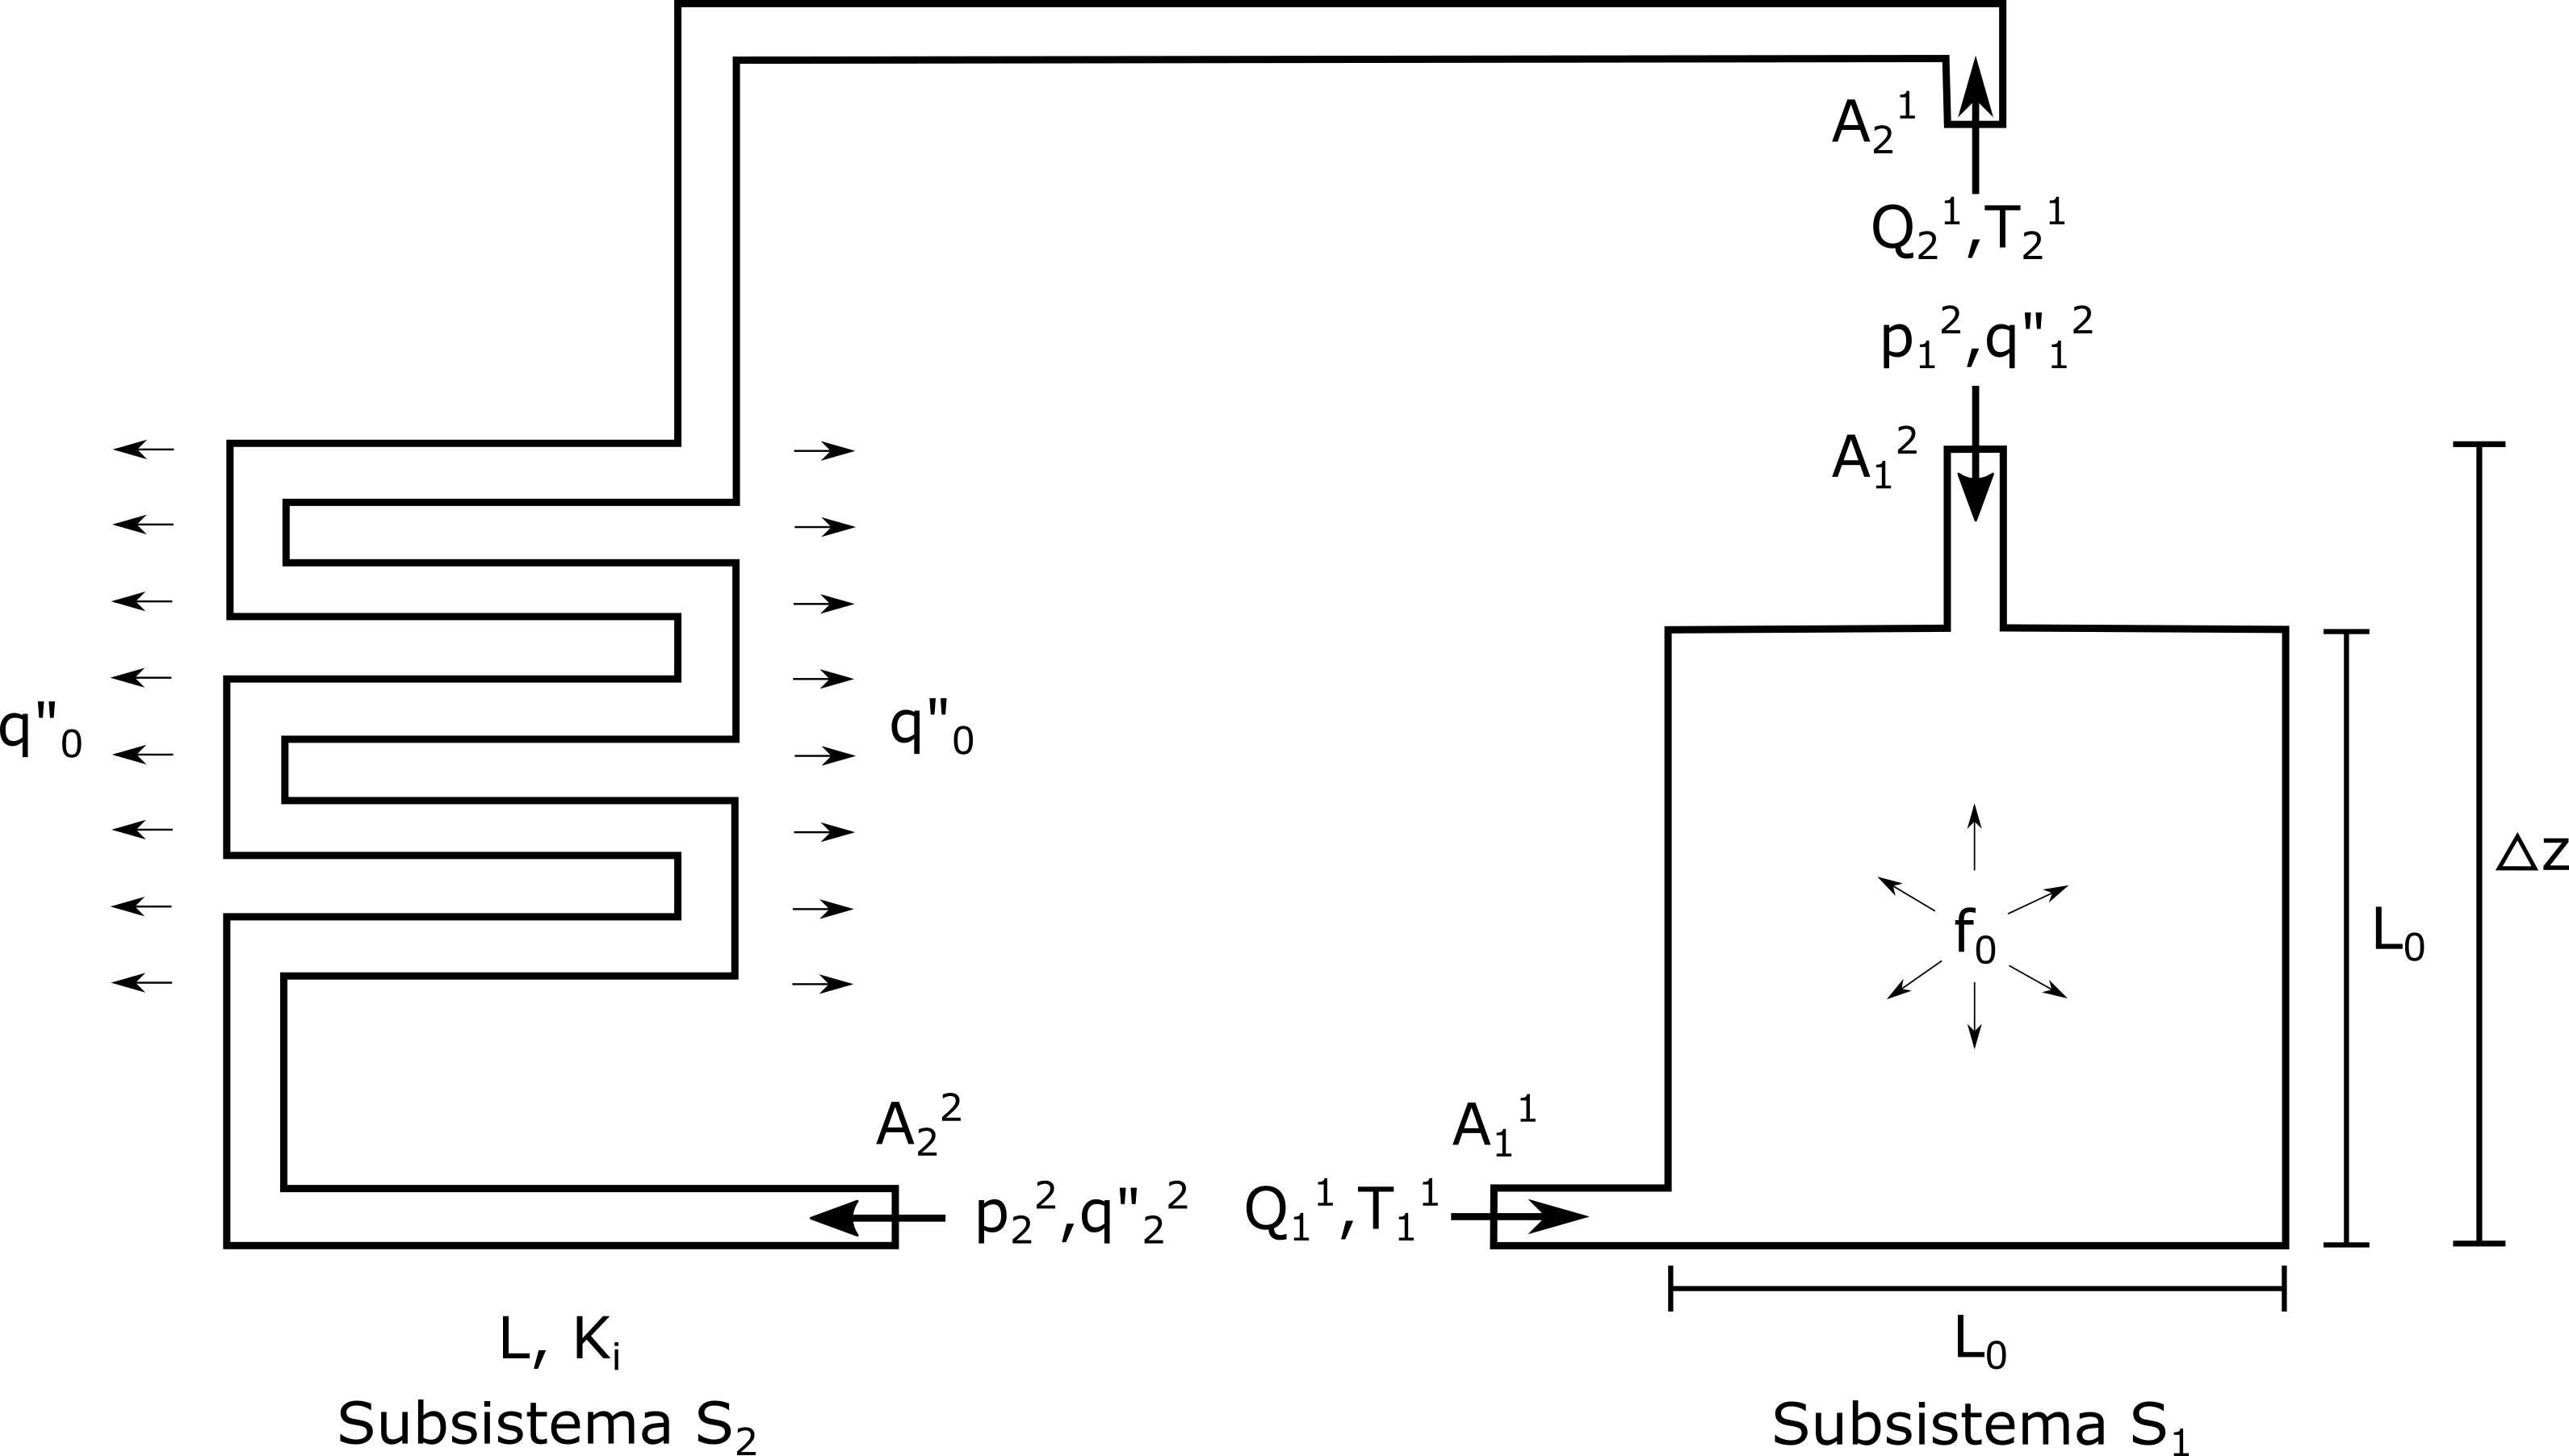
\includegraphics[scale = 0.25]{acople_ri_enief.png}
\caption[Modelo de la fuente fría compuesto por un subsistemas cero-dimensional y otro subsistema bi-dimensional.]
{Modelo de la funete fría analizada. 
El subsistema de la izquierda es un intercambiador de calor y se estudia con un código cero-dimensional.
El modelo de la derecha es una cavidad con una fuente de energía interna y se estudia con un código bi-dimensional.
El sistema completo es abordado con una estrategia de acoplamiento mediante condiciones de borde dinámicas.
En el esquema se ejemplifica una de las elecciones posibles para las variables que son datos en cada subsistema.}
\label{esquemaFuenteFria}
\end{figure}


\subsection*{Subsistemas de estudio}
Los parámetros del modelo del intercambiador de calor son los siguientes:
flujo de calor por unidad de superficie $q_0"=-2\cdot 10^5 W/m^2$, 
longitud de cañerías $L=30$ $m$, 
sumatoria de coeficientes de pérdida de carga concentrada $\sum K_i=1.72$, 
rugosidad de cañerías $\epsilon=0.5\cdot 10^{-3}$ $m$.
Las áreas de las interfaces de acople son $A_2^1=A_2^2=0.03$ $m^2$.
La altura total $\Delta z$ de este subsistema es equivalente a la de la cavidad bidimensional.
El fluido de trabajo es agua ($\rho=10^3$, $c_p=4184$ $J/KgK$).
La evolución de las variables de presión $p$, caudal $Q$ y temperatura $T$ en el subsistema se calcula mediante un código cero-dimensional escrito para este propósito,
que resuelve ecuaciones de pérdida de carga en una red hidráulica con flujo turbulento 
y de transferencia de energía en un intercambiador de calor con flujo constante 
Las ecuaciones del modelo son las siguientes \cite{iedelchik} \cite{kays}:

\begin{equation}
\left\{ \begin{array}{rcl}
p_2^1 + \rho g \Delta z &=& p_2^2 + \rho \frac{1}{2} \left( \frac{Q_1^1}{A_2^1} \right)^2  \left( \frac {f_D L} {D} + \sum_i K_i \right) \\ [0.2cm]
\displaystyle T_2^2 &=& \displaystyle T_2^1 + 2 \frac {q_0" L}{\frac{D}{2} \frac{Q_1^1}{A_2^1}\rho c_p}
\label{eq-intercambiador}
\end{array}
\right.
\end{equation}
donde $p_2^i$ es la presión del subsistema promediada en la interfaz correspondiente,
$Q_2^i$ es el caudal en esta interfaz,
$T_2^i$ es la temperatura promediada en esta interfaz,
$g$ es la aceleración generada por el campo gravitatorio,
$f_D$ es el factor de Darcy de pérdida de carga distribuida,
y $D$ es el diámetro de la tubería.
Notar que el subíndice en cada variable refiere a la numeración global del subsistema, y el supraíndice indica el número de interfaz local,
como se convino previamente en \ref{1:abordaje}.
En este modelo se supone que el flujo de calor es nulo en la dirección axial en cada interfaz de acople.
Esta aproximación es correcta ya que las interfaces se seleccionaron lejos de fuentes y sumideros, donde los gradientes de temperatura son despreciables.
Con este modelo, ninguna de las dos ecuaciones puede recibir valores de contorno \textit{Dirichlet} en ambas interfaces,
ya que los valores de caudal y temperatura en una interfaz determinan el valor en la otra.
Por lo tanto, en la estrategia de acoplamiento, la primera ecuación debe tener, o bien ambos contornos con condiciones de tipo \textit{Neumann}, 
o bien uno con condición de tipo \textit{Neuman} y otro con condición de tipo \textit{Dirichlet}.
La segunda ecuación debe tener uno de los bordes con condición de tipo \textit{Dirichlet} y otro con condición de tipo \textit{Neumann}.
Esta condición es necesaria a pesar de que el flujo de calor recibido no va a ser utilizado, basado en la hipótesis de que es despreciable.
Si el flujo de calor fuera efectivamente apreciable, debería cambiarse el modelo en la ecuación planteada.

La cavidad bidimensional se modela con $L_0=0.3$ $m$, y $A_1^1=A_1^2=0.03$ $m^2$.
Los parámetros del fluido de trabajo son: $\rho_0=10^3$ $Kg/m^3$ a la temperatura de referencia $T_{ref}$,
$\mu=6\cdot 10^{-4}$ $Kg/ms$, $c_p=4184$ $J/KgK$, 
$k=0.64$ $W/mK$ y $\beta=0.44\cdot10^{-3}K^{-1}$.
Se considera que el fluido tiene una fuente interna que se modela como $f_0=10^6$ $W/m^3$.
La evolución de las variables en este subsistema se calcula resolviendo las ecuaciones de Navier-Stokes 
y de transporte de energía.
Se utiliza la aproximación de \textit{Boussinesq} considerando variaciones de densidad solo en el término de fuerza volumétrica.
Las ecuaciones implementadas del modelo son las siguientes \cite{gunzburger} \cite{kays}:

\begin{equation}
\left\{ \begin{array}{rcl}
\displaystyle \frac {\partial \bar{u}}{\partial t} + ( \bar{u} \cdot \nabla) \bar{u}  + \frac {\nabla p}{\rho_0} - 
\nabla \cdot \left[ \left( \nu + \nu_T \right) \left( \nabla \bar{u} + \nabla \bar{u}^T \right) \right] && \\
- \left( 1- \beta (T-T_{ref}) \right)\bar{g} &=& 0 \\ [0.2cm]
\nabla \cdot \bar{u} &=& 0 \\ [0.2cm]
\displaystyle \frac {\partial T}{\partial t} + ( \bar{u} \cdot \nabla) T =0 - \frac {k}{\rho_0 c_p} \Delta T &=& \displaystyle \frac{f_0}{\rho_0 c_p}
\label{eq-cavidad}
\end{array}
\right.
\end{equation}
donde $\bar{u}$ es el campo de velocidades dentro de la cavidad,
$p$ el campo de presiones y
$T$ el campo de temperaturas.

Las ecuaciones (\ref{eq-cavidad}) se resuelven mediante la formulación \textit{Petrov-Galerkin} \cite{galerkin} de elementos finitos, 
con elementos lineales para aproximar los campos de presiones, velocidades y temperaturas, 
estabilizando con los métodos \textit{SUPG} \cite{supg} y \textit{PSPG} \cite{pspg}.
El método \textit{SUPG} (\textit{Streamline Upwind Petrov-Galerkin}) se utiliza para estabilizar problemas de transporte con alto número de \textit{Peclet} (\textit{Pe}).
El \textit{Pe} es un número adimensional que relaciona la velocidad de advección de un flujo y la velocidad de difusión, y está relacionado con el número de \textit{Reynolds} (\textit{Re}).
En las ecuaciones de \textit{Navier-Stokes}, el método estabiliza las evoluciones con alto \textit{Re},
y consiste en la adición de una difusividad extra en la dirección de las líneas de corriente.
El método \textit{PSPG} (Pressure Stabilizing Petrov-Galerkin) se utiliza para evadir la condición \textit{LBB}\footnote{
La condición \textit{Ladyzhenskaya-Babuska-Breezi (LBB)} o \textit{inf-sup}
es una condición necesaria y suficiente para que el problema de \textit{Stokes}
discretizado mediante algún método \textit{Galerkin}
quede bien planteado.
},
que básicamente impone restricciones sobre los espacios de elementos utilizados.

En las paredes se imponen condiciones de no deslizamiento para las ecuaciones de \textit{Navier-Stokes} y de flujo de energía nulo para la ecuación de energía.
En las interfaces de acople, deben definirse una serie de condiciones de borde.
En las ecuaciones de \textit{Navier-Stokes}, en cada interfaz pueden setearse valores de velocidades normales, suponiendo velocidades tangenciales nulas (bajo la hipótesis de flujo paralelo),
o valores de fuerzas normales (presión), suponiendo que las fuerzas tangenciales son nulas.
En la ecuación de energía, cada borde necesita o bien un perfil de temperaturas o bien un perfil de flujo de calor.
Los cálculos se realizaron implementando diferentes estrategias y verificando que los mismos convergieran.

La malla de cálculo se genera con \textbf{Gmsh} \cite{gmsh} y se discretiza el dominio en $43874$ elementos triangulares
con un tamaño medio de arista de $\Delta x \approx 0.005m$.
El cálculo se realiza con \textbf{Par-GPFEP} \cite{gpfep} \cite{pargpfep}.
Las modificaciones de \textbf{Par-GPFEP} que fueron necesarias para implementar el acoplamiento son comentadas en el Apéndice \ref{C:pargpfep}.


\subsection*{Estrategia de resolución}

En cada interfaz de acople existen incógnitas de velocidades, fuerzas, temperatura y flujo de calor.
En el caso de las velocidades la estrategia implementada es definir una variable integral, 
el caudal volumétrico $Q$, que servirá como una de las variables de acoplamiento\footnote{
Cuando se utilizan variables integrales o promediadas para el acoplamiento, es necesario definir una estrategia extra en el subdominio que la recibe.
Como cada subproblema solo queda bien definido si la condición de borde está dada sobre todos los puntos del borde, estos valores deben distribuirse considerando algún perfil.
Por ejemplo, para el caso del subdominio que recibe un valor de caudal, y está modelado con ecuaciones bi-dimensionales, necesita definir un perfil de velocidades a lo largo de toda la sección de acople.
La definición del perfil se basa en alguna hipótesis que el modelador considera adecuada conforme a la física del problema.
Este paso debe analizarse con cuidado ya que los resultados del acoplamiento dependen de ello.
}.
En el caso de las fuerzas se utilizan valores promediados para la fuerza normal (presión $p$).
Las fuerzas tangenciales se consideran nulas bajo la hipótesis de que son despreciables en las interfaces de acople.
Esta hipótesis es correcta cuando el flujo es paralelo, 
y por ello se selecciona como interfaz de acople aquella que se corresponda con el perfil de velocidades lo más plano posible, lejos de las curvas.
Los valores de temperatura de acople también corresponden a valores $T$ promediados en la interfaz,
y el flujo de calor $q''$ de acople corresponde al flujo integral a través de ella.
En los subsistemas bi-dimensionales, los perfiles de velocidadades y temperaturas construidos a partir de las variables recibidas se consideran planos,
bajo la hipótesis de flujo paralelo.
Con esta estrategia, existen cuatro incógnitas en cada interfaz de cada subsistema. 
Considerando los dos subsistemas, existen en total dieciseis incógnitas.

El sistema de ecuaciones de incógnitas queda definido por ocho ecuaciones de continuidad de variables \ref{continuidad}
y otras ocho ecuaciones modelos \ref{ecuaciones-modelos} que todavía deben ser seleccionadas.
Las ecuaciones de continuidad en las interfaces implican que:

\begin{equation}
\left\{ \begin{array}{rcl}
Q_1^1&=& Q_2^2 \\
Q_1^2&=& Q_2^1 \\
p_1^1&=& p_2^2 \\
p_1^2&=& p_2^1 \\
T_2^1&=& T_2^2 \\
T_2^2&=& T_2^1 \\
q"_2^1&=& - q"_2^2 \\
q"_2^2&=& - q"_2^1
\end{array}
\right.
\end{equation}

Las ecuaciones modelos deben ser seleccionadas en base a la combinación de condiciones de borde propuesta para resolver el acoplamiento.
Independientemente de cuál fuera ésta,
para que el problema quede bien planteado debe serleccionarse solo una de las relaciones para el par \textit{presión-caudal}
y solo una para el par ºtextit{temperatura-flujo de calor} en cada interfaz.
Así entonces, considerando las dos interfaces del subsistema 1 se generan cuatro ecuaciones de residuos:

\begin{equation}
\left\{ \begin{array}{rcl}
(R_{p,Q})_{1}^{1}  \;(Q_1^1, p_1^1, T_1^1, Q_1^2, p_1^2, T_1^2) &=& 0 \\
(R_{T,q"})_{1}^{1} \;(Q_1^1, T_1^1, q"_1^1, Q_1^2, T_1^2, q"_1^2) &=& 0 \\
(R_{p,Q})_{1}^{2}  \;(Q_1^1, p_1^1, T_1^1, Q_1^2, p_1^2, T_1^2) &=& 0 \\
(R_{T,q"})_{1}^{2} \;(Q_1^1, T_1^1, q"_1^1, Q_1^2, T_1^2, q"_1^2) &=& 0 
\end{array}
\right.
\label{residuos-1}
\end{equation}
donde $(R_{p,Q})_1^i$ es el residuo del par \textit{presión-caudal} en la interfaz $i$ y
$(R_{T,q''})_1^i$ es el residuo del par \textit{temperatura-flujo de calor} en la interfaz $i$.
Entre las dos interfaces del subsistema 2 se generan otras cuatro ecuaciones de residuos:

\begin{equation}
\left\{ \begin{array}{rcl}
(R_{p,Q})_{2}^{1}  \;(Q_2^1, p_2^1, T_2^1, Q_2^2, p_2^2, T_2^2) &=& 0 \\
(R_{T,q"})_{2}^{1} \;(Q_2^1, T_2^1, q"_2^1, Q_2^2, T_2^2, q"_2^2) &=& 0 \\
(R_{p,Q})_{2}^{2}  \;(Q_2^1, p_2^1, T_2^1, Q_2^2, p_2^2, T_2^2) &=& 0 \\
(R_{T,q"})_{2}^{2} \;(Q_2^1, T_2^1, q"_2^1, Q_2^2, T_2^2, q"_2^2) &=& 0
\end{array}
\right.
\label{residuos-2}
\end{equation}
Notar que según la estrategia de acoplamiento seleccionada, algunas de las dependencias pueden anularse.
En la Figura \ref{esquemaFuenteFria} se presenta una estrategia en la que las condiciones de borde dinámicas son 
de tipo de tipo Dirichlet para la interfaz inferior de la cavidad y la interfaz superior del intercambiador de calor, 
y de tipo de tipo Neumann para las restantes.

Como el circuito es cerrado es necesario proveer un valor de referencia para la presión.
En la formulación desarrollada se fija un valor de presión aritrario en la interfaz superior del intercambiador de calor,
por lo que la ecuación $(R_{p,Q})_{2}^{1}=0$ queda descartada, y es sustituida por la siguiente:

\begin{equation*}
p_2^1 = 0.
\end{equation*}

El programa \textit{maestro} utilizado es \textbf{Coupling}.
La comunicación entre códigos se da por MPI en modo SISD.
Como se mencionó en \ref{1:evolucion}, no existe necesidad de que ambos códigos utilicen el mismo paso temporal de cálculo.
Sin embargo en ambos modelos se utiliza $\Delta t=0.01s$, debido a que ninguno requiere una mayor discretización temporal.

\subsection*{Resultados del cálculo}

\begin{figure}[ht]
	\begin{minipage}{0.5\linewidth}
		\centering
		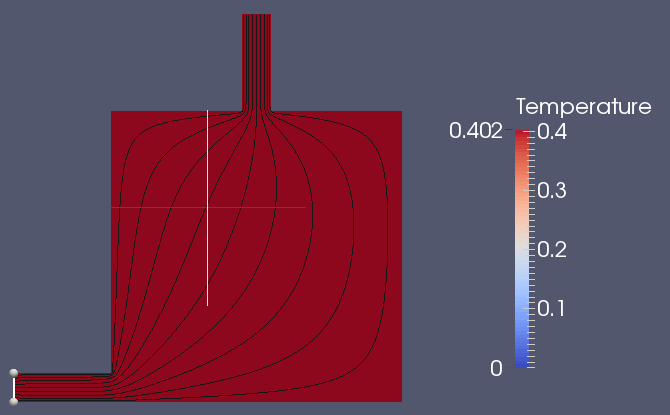
\includegraphics[scale=0.32]{acople_ri28_t0.png}
		\caption[]{t=0 s}
		\label{asd}	
	\end{minipage}
	\begin{minipage}{0.5\linewidth}
		\centering
		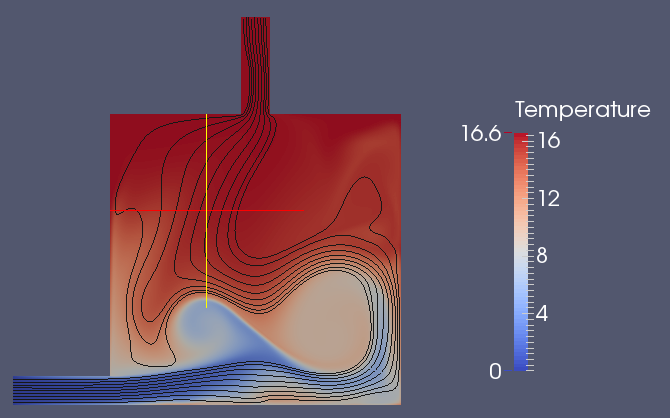
\includegraphics[scale=0.315]{acople_ri28_t40.png}
		\caption[]{t=40 s}
		\label{asd}	
	\end{minipage}
	\caption[Evolución en el transitorio inicial del fluido dentro de la cavidad bidimensional con fuente interna]
  {Evolución del fluido dentro de la cavidad bidimensional con fuente interna.
	El número de Richardson del fluido $Ri=28.34$.
	Pueden apreciarse las líneas de corriente que se establecen al comienzo de la simulación.} 
	\label{acople_ri28_1}
\end{figure}

\begin{figure}[ht]
	\begin{minipage}{0.5\linewidth}
		\centering
		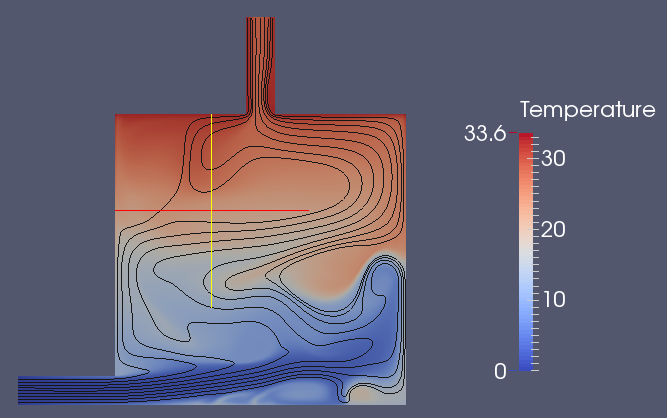
\includegraphics[scale=0.32]{acople_ri28_t80.png}
		\caption[]{t=80 s}
		\label{asd}	
	\end{minipage}
	\begin{minipage}{0.5\linewidth}
		\centering
		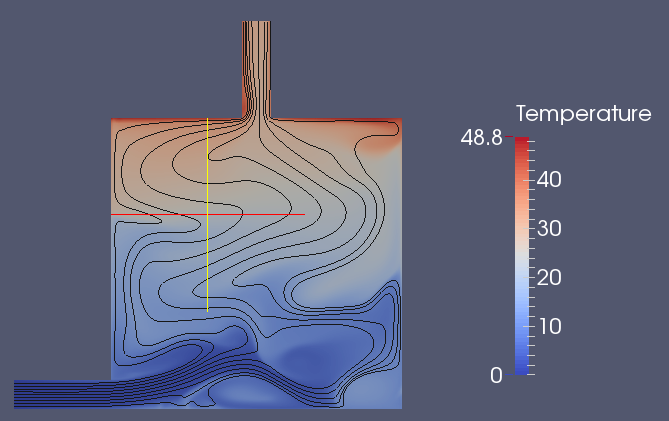
\includegraphics[scale=0.315]{acople_ri28_t250.png}
		\caption[]{t=250 s}
		\label{asd}	
	\end{minipage}
	\caption[Evolución hacia el estado estacionario del fluido dentro de la cavidad bidimensional con fuente interna]
  {Evolución del fluido dentro de la cavidad bidimensional con fuente interna.
	El número de Richardson del fluido $Ri=28.34$.
	Pueden apreciarse las líneas de corriente serpenteantes y la estratificación del fluido alcanzando un estado estacionario.}  
	\label{acople_ri28_2}
\end{figure}

Las condiciones iniciales del sistema son estáticas y sin gradientes de temperatura.
A medida que evoluciona el fluido comienza a incrementar su temperatura en la cavidad y a circular por fuerza boyante.
El régimen del fluido depende del número adimensional de Richardson \textit{Ri}, \cite{richardson},
que representa la relación entre las fuerzas boyantes y las fuerzas inerciales.
Con los parámetros del subsistema bidimensional el \textit{Ri} del fluido queda definido en $Ri=28.34$.
Como este valor es alto, el fluido se estratifica en capas de diferentes temperaturas.
Las líneas de corrientes serpentean entre la entrada y la salida, manteniendo corrientes paralelas horizontales.
En las Figuras \ref{acople_ri28_1} y \ref{acople_ri28_2} puede observarse 
la evolución de las líneas de corriente y del campo de temperatura en la cavidad bidimensional.

\subsection*{Análisis de métodos de resolución del sistema de ecuaciones de residuos}

Se exploran diferentes métodos numéricos para resolver el acoplamiento presentado en las ecuaciones \ref{residuos-1} y \ref{residuos-2}.
El parámetro de interés aquí no es la cantidad de iteraciones de cada método sino la cantidad de evaluaciones de funciones que cada uno requiere,
ya que el tiempo de cálculo está directamente relacionado con ellas.
En la Figura \ref{iteraciones_ri} puede apreciarse la cantidad de evaluaciones requeridas 
por cada método para disminuir los residuos debajo de cierta tolerancia prefijada, para cada paso temporal.
El método de \textit{Newton} calcula la matriz jacobiana en cada iteración.
Este cálculo se realiza con diferencias finitas a primer órden y por lo tanto requiere 1 evaluación de los residuos en el punto inicial,
y 8 evaluaciones extras para el cálculo de cada diferencia finita.
En total son 9 evaluaciones extras.
Puede observarse que la cantidad de iteraciones del método para converger es en promedio una sola, ya que en general utiliza 10 evaluaciones en cada paso temporal.

\begin{figure}[ht]
\centering{}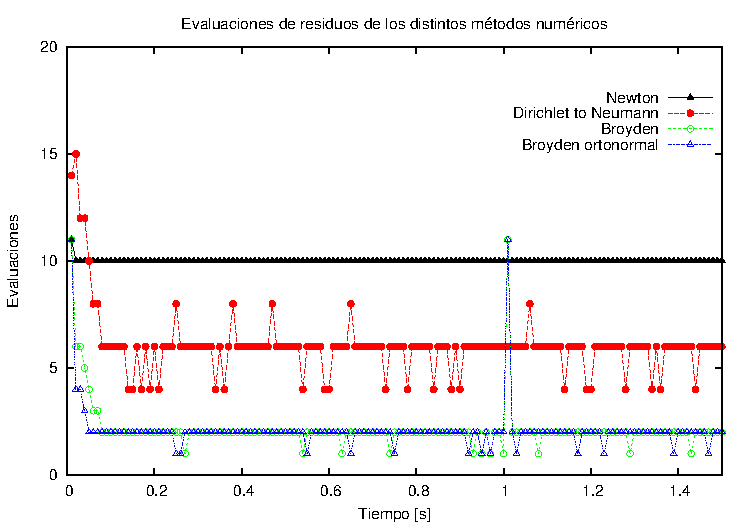
\includegraphics[scale = 1]{evaluaciones-ff.pdf}
\caption
{Evaluaciones de residuos requeridas por diversos métodos numéricos para resolver los sistemas de ecuaciones planteados
 en el problema doblemente acoplado descripto de la fuente fría de neutrones.} \label{iteraciones_ri} 
\end{figure}

Los métodos \textit{quasi-Newton} inicializan la matriz jacobiana sólo en el primer paso temporal,
y luego utilizan aproximacionas económicas de la misma. 
Cada cierta cantidad de pasos temporales pueden reinicializar la matriz también mediante diferencias finitas. 
En los modelos realizados se utiliza reinicialización cada 100 pasos temporales, 
y por lo tanto la primera reinicialización se efectúa en el paso 101.
En promedio estos métodos requieren dos iteraciones por cada paso temporal, 
además de las 9 llamadas extras a códigos en cada paso de reinicialización.
Los métodos \textit{Broyden} y \textit{Broyden ortonormal} tinen comportamiento similar y demuestran ser más eficientes que el método clásico.
El método \textit{Dirichlet-to-Neumann} es el que mayor cantidad de iteraciones necesita por cada paso temporal, 
excediendo el doble de los pasos requeridos por los métodos \textit{quasi-Newton}.

\section{Análisis del segundo sistema de parada de un reactor de investigación}
\label{3:mockup}

\subsection*{Presentación del problema}
El Departamento de Mecánica Computacional de CNEA tuvo a cargo el análisis del segundo sistema de parada (SSP) del reactor RA-10 \cite{ra10}.
El RA-10 es un reactor de investigación multipropósito, destinado principalmente a aumentar la producción de radioisótopos para uso de diagnóstico de enfermedades,
a la investigación científica de haces de neutrones en diferentes rangos de energía,
y al ensayo de materiales.
El RA-10 es un reactor de pileta abierta de flujo ascendente, con combustibles de bajo enriquecimiento tipo placa y agua liviana como refrigerante.
El núcleo del reactor está inmerso en un tanque que contiene agua pesada como material reflector.
El SSP consiste en el accionamiento del vaciado de este tanque.
El drenado del agua pesada disminuye drásticamente la reactividad, apagando el reactor.
La tarea de estudio consistió en verificar si el diseño cumple con el criterio de éxito,
a saber, completar el 55\% del vaciado en un tiempo inferior a los 15 segundos,
ante una falla simple del sistema (falla de apertura de cualquiera de las válvulas).
Este requerimiento pudo verificarse tras el análisis \cite{cnea-informe-ra10}.

\begin{figure}[ht]
\centering{}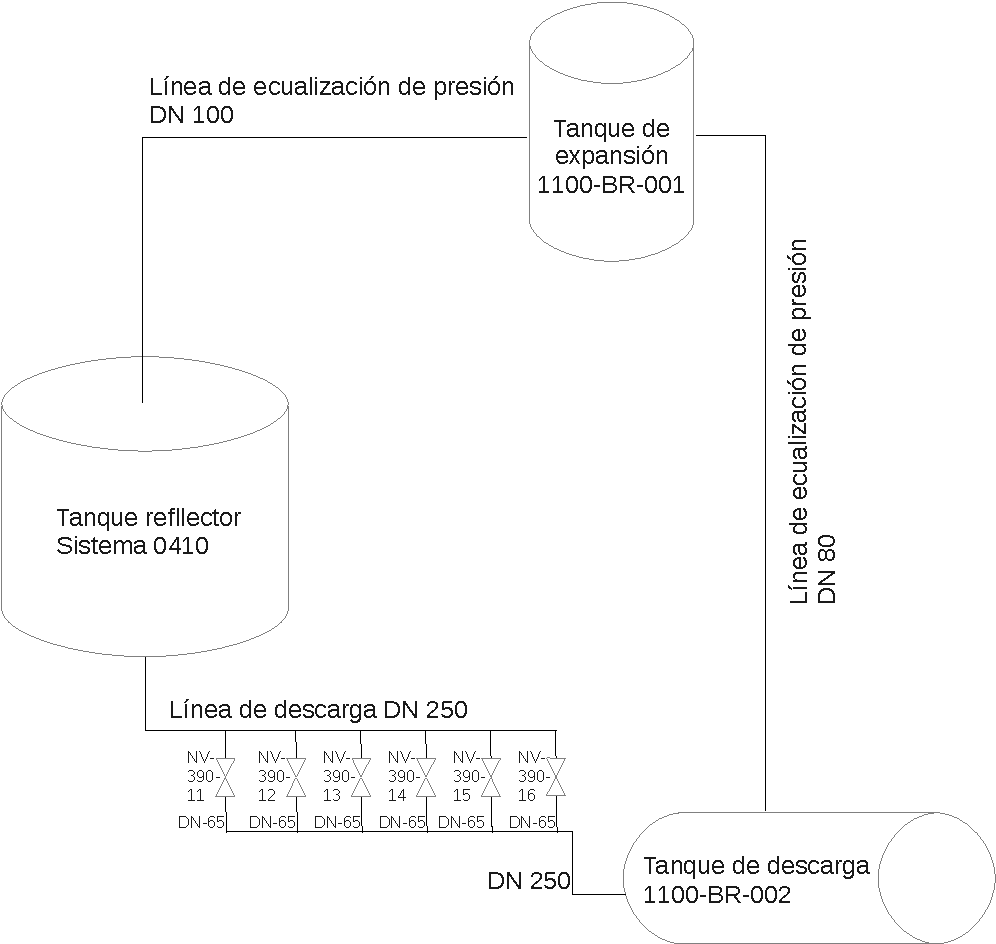
\includegraphics[scale = 0.8]{SSP.pdf}
\caption{Esquema del segundo sistema de parada del reactor RA10.} \label{fig:SSP} 
\end{figure}

La Figura \ref{fig:SSP} esquematiza el SSP. 
En el mismo pueden destacarse tres grandes subsistemas: el tanque del reflector, la red hidráulica de descarga y
la red hidráulica de ecualización de presiones. 
En operación normal del reactor las
válvulas que pueden observarse en la red hidráulica permanecen cerradas, y el agua pesada rellena las cañerías y el tanque de reflector. 
El resto del sistema es rellenado con gas Helio, excepto una porción del tanque de expansión que también permanece rellena con líquido. 
Cuando es accionado el SSP se abren las válvulas y el líquido comienza a drenar hacia el tanque de descarga, acelerado por la fuerza gravitatoria. 
Asimismo, el Helio circula en el mismo sentido en el resto del sistema, rellenando el volumen desplazado de líquido.

El análisis del problema completo hubiera demandado elevados recursos computacionales debido a los requerimientos de malla.
Por ello se propuso desarrollar un modelo multiescala del sistema,
desacoplándolo en subsistemas que pudieron estudiarse por separado con estrategias de acoplamiento mediante condiciones de borde apropiadas.
El SSP del RA10 se dividió en tres subsistemas:

\begin{itemize}
\item Subsistema del tanque del reflector,
\item Subsistema de la red hidráulica de descarga,
\item Subsistema de la red hidráulica de ecualización de presiones.
\end{itemize}

En el trabajo presentado los subsistemas se acoplaron mediante una estrategia de acoplamiento débil \cite{ra10-paper} \cite{ra10-enief}.

Previo a este trabajo, se realizaron tareas de validación de las herramientas de cálculo.
Para ello se estudió un sistema similar para el que se conocían datos experimentales de tiempo de vaciado.
Estos datos sirvieron para contrastar los resultados obtenidos con las herramientas de cálculo.
El sistema analizado fue el \textit{mockup} del SSP del reactor OPAL \cite{invap-mockup},
montado por INVAP en San Carlos de Bariloche.
Debido a que el \textit{mockup} del SSP del OPAL está abierto a la atmósfera,
no cuenta con línea de ecualización de presiones y por lo tanto ésta no se consideró en el modelo.
En un estudio \cite{cnea-informe-mockup} se analizó el detalle fluídico tridimensional en el tanque reflector durante la descarga,
modelando con ecuaciones cero-dimensionales la pérdida de carga en la red hidráulica 
y acoplando los subsistemas de forma débil.
El estudio que a continuación se presenta es otro estudio que analiza con mayor detalle la distribución de caudales a través del arreglo de válvulas,
modelando el comportamiento del resto del sistema con ecuaciones cero-dimensionales,
y acoplando los subsistemas de forma fuerte, con la estrategia descripta en los dos primeros capítulos.
El propósito de este estudio es investigar si existe algún efecto en las cañerías que podría no estar siendo considerado en el otro modelo.

\subsection*{Subsistemas de estudio}

Se proponen dos subsistemas de estudio:
el primero incluye el tanque del reflector acoplado a una porción de la red hidráulica en la descarga,
y el segundo modela el arreglo de válvulas.

El primer subsistema se analiza con ecuaciones cero-dimensionales,
realizando balances de masa y energía.
La evolución de la altura $h$ de la superficie libre en el tanque del reflector
queda modelada a través de la siguiente ecuación \cite{bird}:

\begin{equation}
\ddot{h} h + \frac{\dot{h}^2}{2}\left( 1- \left(\frac{A_T}{A_D} \right)^2 \right) + g \Delta h_{red} + \ddot{h}  l_D = 
\frac{p_{atm}-p_1^1}{\rho} + \Delta \hat{u}
\label{eq-tanque}
\end{equation}
donde $p_1^1$ es la presión en la interfaz de acople,
$A_T$ es la área transversal del tanque del reflector, 
$A_D$ es la sección transversal de la línea de descarga,
$\Delta h_{red}$ es la altura total de la columna de líquido en el subsistema,
$l_D$ es la longitud total de cañerías en el subsistema,
$p_{atm}$ es la presión sobre la superficie libre,
y $\rho$ es la densidad del agua.
$\Delta u$ representa la pérdida de carga por unidad de masa y puede modelarse como:

\begin{equation}
\Delta u = \frac {1} {2} {v_D}^2 \left( \frac {f_D l_D}{D} + \sum_i K_i \right)
\end{equation}
donde $v_D$ es la velocidad del fluido en la línea de descarga,
(que puede escribirse en términos de $\dot{h}$),
$\frac {f_D*l_D}{D}$ es el factor de pérdida de carga distribuida en las tuberías,
(en función del factor de Darcy $f_D$, la longitud de tuberías $l_D$ y el diámetro de las mismas $D$)
y $\sum_i K_i$ es la sumatoria de factores de pérdida de carga concetrada.

La Tabla \ref{tabla-tanque} reúne los parámetros del subsistema.
Los datos geométricos pueden consultarse en las referencias \cite{invap-mockup}.
El factor de pérdida de carga concentrada fue calculado en función de estos datos geométricos \cite{iedelchik},
e incluye la contracción abrupta en la unión entre el tanque y la red hidráulica,
y tres codos de 90º presentes en ella, previos al arreglo de válvulas.

\begin{table}[]
\centering
\begin{tabular}{|l|l|}
\hline
Parámetro        & Valor          \\ \hline
$A_T$            & 5.30 $m^2$     \\ \hline
$A_D$            & 0.05 $m^2$     \\ \hline
$\Delta h_{red}$ & $h$ + 4.98 $m$ \\ \hline
$l_D$            & 11.98 $m$      \\ \hline
$p_{atm}$        & 92000 $Pa$     \\ \hline
$\rho$           & 998 $Kg/m^3$   \\ \hline
$D$              & 0.254 $m$      \\ \hline
$\sum_i K_i$     & 1.13           \\ \hline
\end{tabular}
\caption{Parámetros del subsistema del tanque del reflector con acople de sección de red hidráulica}
\label{tabla-tanque}
\end{table}

Una vez resuelta la ecuación (\ref{eq-tanque}) para un dado valor de tiempo,
el caudal de descarga $Q_1^1$ puede calcularse simplemente como:

\begin{equation}
Q_1^1 = -\dot{h} A_D
\label{eq-qd}
\end{equation}
Todos estos cálculos se realizan con un programa escrito para este propósito.

El subsistema arreglo de válvulas es modelado con una malla tridimensional de elementos tetraédricos realizada en \textbf{Salomé} \cite{salome}.
El caudal ingresa a través del extremo superior y se reparte entre los múltiples caños que comunican los colectores.
En operación normal del reactor cada uno de ellos está bloqueado mediante una válvula esférica,
y del otro lado las cañerías están rellenas de gas,
pero durante el accionamiento del sistema de parada las mismas se abren dejando pasar libremente al fluido.
Las válvulas esféricas instaladas no presentan pérdidas de carga concentrada y por lo tanto no son modeladas.
Como es de interés el análisis ante falla simple del sistema,
se supone que una de las válvulas no abre y por ello ese caño tampoco se modela.
En los primeros cálculos se supone que la válvula en falla es la ubicada en la última rama del arreglo.
Como otra simplificación del problema se supone que inicialmente el agua rellena todas las cañerías en forma estática.
Más adelante se estudia la validez de éstas aproximaciones.
Los datos dimensionales de las cañerías pueden consultarse en las referencias \cite{invap-mockup}.

Debido a que el régimen del fluido es turbulento durante la mayor parte de la descarga,
y una simulación Simulación Numérica Directa (DNS, por sus siglas en inglés) demandaría elevados recursos computacionales,
se utiliza un modelo de turbulencia de tipo Promedio de Reynolds de Navier-Stokes (RANS, por sus siglas en inglés)
para modelar la fricción interna del fluido.
El modelo utilizado es el modelo $\kappa-\epsilon$ \textit{realizable} \cite{k-e-realizable},
en el que las ecuaciones se estabilizan mediante un método de control de coeficientes.
El sistema de ecuaciones resultantes en el segundo subsistema es:

\begin{equation}
\left\{ \begin{array}{rcl}
\displaystyle \frac{\partial \bar{U} }{\partial t} + ( \bar{U} \cdot \nabla) \bar{U} + \frac {\nabla P^*}{\rho} - 
\nabla \cdot \left[ \left( \nu + \nu_T \right) \left( \nabla \bar{U} + \nabla U^T \right) \right] -\bar{f} &=& 0 \\
\nabla \cdot \bar{U} &=& 0 \\
\displaystyle \nu_T -c_\mu \frac{\kappa^2}{\epsilon} &=& 0\\
\displaystyle \frac{\partial \kappa}{\partial t} + ( \bar{U} \cdot \nabla) \kappa - \frac{c_\mu} {2}{\kappa^2}{\epsilon} \left | \nabla \bar{U} + \nabla\bar{U}^T \right | ^2  
- \nabla \cdot \left( c_\mu \frac{\kappa^2}{\epsilon} \nabla \kappa \right) + \epsilon &=& 0 \\
\displaystyle \frac{\partial {\epsilon}}{\partial t} + ( \bar{U} \cdot \nabla) \epsilon - \frac{c_1} {2} \kappa \left | \nabla \bar{U} + \nabla \bar{U}^T \right | ^2
- \nabla \cdot \left( c_{\epsilon} \frac{\kappa^2}{\epsilon} \nabla \epsilon \right) + c_2 \frac{\epsilon}{\kappa} &=& 0
\label{eq-mani}
\end{array} \right.
\end{equation}
donde $\bar{f}$ es una fuerza volumétrica, 
$\kappa$ es la energía cinética turbulenta, $\epsilon$ es la disipación viscosa de energía turbulenta,
$\nu_T$ es la viscosidad turbulenta y $P^*$ es la presión efectiva del sistema, que se calcula como
$\displaystyle P^* = P + \frac {2}{3}\kappa$.
Las variables mayúsculas refieren a valores medios estadísticos.
Los parámetros de las ecuaciones de transporte de $\kappa$ y $\epsilon$ toman los siguientes valores:
$c_\mu=0.09$, $c_1=0.126$, $c_2=1.92$ y $c_\epsilon=0.07$ \cite{durbin}.

En las ecuaciones de \textit{Navier-Stokes}, cada borde necesita un perfil de velocidades normales o de fuerzas normales,
y otro de velocidades tangenciales o de fuerzas tangenciales \cite{gunzburger}.
Si la condición de borde de ingreso de la cañería es el valor del caudal $Q_2^1$,
a partir de éste puede definirse un perfil de velocidades del fluido.
El regímen de flujo es turbulento durante la mayor parte de la descarga y por tanto este perfil puede suponerse plano.
En base a estas velocidades puede calcularse un valor para la intensidad turbulenta $I_T$,
y con ella aproximarse los valores de $\kappa$ y $\epsilon$ en la interfaz.
Si la condición de borde de ingreso a la cañería es el valor de presión media,
la intensidad turbulenta $I_T$ en cada paso de evolución temporal puede calcularse de forma aproximada a partir de la solución para el caudal en el paso previo.
En la descarga de la cañería se impone una fuerza normal que depende de la presión atmosférica,
despreciando las fuerzas tangenciales.
Las ecuaciones de $\kappa$ y $\epsilon$ no requieren condiciones de contorno en esta interfaz.
Para evitar la resolución de la capa límite en las paredes de las tuberías se implementa un modelo de pared,
en el que se reemplaza la misma por una tracción tangencial equivalente a la que realizaría la misma sobre la corriente externa
\cite{k-e}.
Este modelo impone condiciones de tipo \textit{Dirichlet} para $\kappa$ y $\epsilon$ en la frontera en que se impone la ley de pared.

El sistema de ecuaciones (\ref{eq-mani}) es resuelto en pasos fraccionados \cite{lew} mediante la formulación \textit{Petrov-Galerkin} \cite{galerkin} de elementos finitos con elementos lineales, 
estabilizada mediante \textit{SUPG} \cite{supg} y \textit{PSPG} \cite{pspg}.
En el primer paso fraccionado se resuelve el transporte de $\kappa$,
en el segundo paso se resuelve el transporte de $\epsilon$,
y en el último paso se resuelven en forma monolítica las ecuaciones de \textit{Navier-Stokes}.

Una vez resueltas las ecuaciones,
si la condición de borde en la interfaz de acople $I_2^1$ había sido el caudal $Q_2^1$,
es posible calcular el valor de la presión promedio $<p_2^1>$ en esta interfaz
a partir de los valores $<P^*_{I_2^1}>$ y $<\kappa_{I_2^1}>$ promediados en ella:

\begin{equation}
<p_2^1> = <P^*_{I_2^1}> - \frac {2}{3} <\kappa_{I_2^1}>
\end{equation}

Si la condición de borde en la interfaz de acople hubiera sido la presión promedio $<p_2^1>$,
el caudal $Q_2^1$ se calcula simplemente mediante integración numérica del campo de velocidades en los nodos de la interfaz.

Todos estos cálculos se realizan con \textbf{Par-GPFEP}.

\subsection{Estrategia de resolución}

Los dos subsistemas están conectados a través de una sección de la tubería,
en la cual quedan acoplados los valores de velocidades y fuerzas.
La estretegia implementada es similar a la utilizada en \ref{3:ff} y consiste en utilizar como variables de acoplamiento el caudal volumétrico $Q$ y la presión promedio $p$.
Las fuerzas tagenciales se consideran nulas.
A fines de cumplir con esta hipóteisis, la interfaz de acople se selecciona lejos de los codos.
El subsistema tanque del reflector tiene como incógnitas la presión $p_1^1$ y el caudal $Q_1^1$ en la interfaz de acople $I_1^1$.
Asimismo, el subsistema arreglo de válvulas tiene como incógnitas $p_2^1$ y $Q_2^1$ en $I_2^1$.
Las ecuaciones de continuidad implican que:

\begin{equation}
\left\{ \begin{array}{rcl}
p_1^1 &=& p_2^1 \\
Q_1^1 &=& Q_2^1
\end{array}
\right.
\end{equation}

Se utiliza la siguiente estrategia:
condiciones de borde de tipo \textit{Neumann} en la interfaz de acople para el subsistema tanque del reflector,
y condiciones de borde de tipo \textit{Dirichlet} para el subsistema arreglo de válvulas\footnote{
Se podrían haber definido otras estrategias.
La estrategia implementada permite resolver las ecuaciones en ambos subdominios de una forma cómoda.
En el modelo tri-dimensional, por ejemplo, el valor de caudal recibido es útil para construir valores para las condiciones de borde del modelo turbulento utilizado.
}.
En base al caudal recibido en este subsistema se calcula un perfil de velocidades.
Las ecuaciones de residuos quedan entonces:

\begin{equation}
\left\{ \begin{array}{rcl}
(R_{p,Q})_{1}^{1}  \;(p_1^1) &=& 0 \\
(R_{p,Q})_{2}^{1}  \;(Q_2^1) &=& 0
\end{array}
\right.
\end{equation}

El programa \textit{maestro} utilizado es \textbf{Coupling}.
La comunicación entre códigos se da por MPI en modo SIMD.

\subsection*{Evolución de la descarga del SSP}

Se realizan cálculos utilizando mallas del modelo tri-dimensional con diferente refinamiento para estudiar la convergencia de los resultados.
La primera es una malla con $\Delta x=0.01m$ y 1145659 de elementos. 
La segunda es malla tiene $\Delta x=0.008m$ y 1806202 elementos.
La tercera es la malla más fina y tiene $\Delta x=0.005m$ y 2951259 elementos.
Se utiliza $\Delta t=0.01s$ en los cálculos con las dos primeras mallas y $\Delta t=0.005s$ en los cálculos con la última malla.
Las ecuaciones de residuos se resuelven
mediante el método de \textit{Broyden ortonormal},
con reinicialización de la matriz jacobiana cada 100 pasos temporales.
En la Figura \ref{qpvst} se reportan los resultados obtenidos para la evolución de los caudales y de las presiones en la interfaz de acople.

\begin{figure}[ht]
	\begin{minipage}{0.5\linewidth}
		\centering
		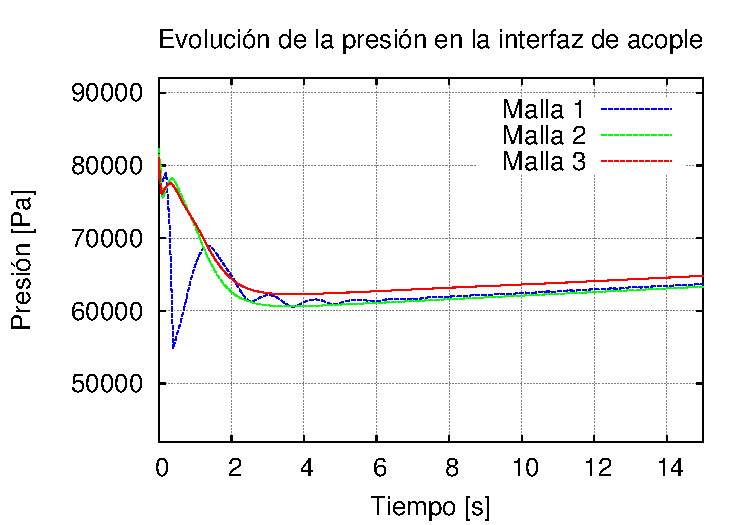
\includegraphics[scale=0.55]{p_vs_t.pdf}
		%\caption{t=80 s}
		\label{asd}	
	\end{minipage}
	\begin{minipage}{0.5\linewidth}
		\centering
		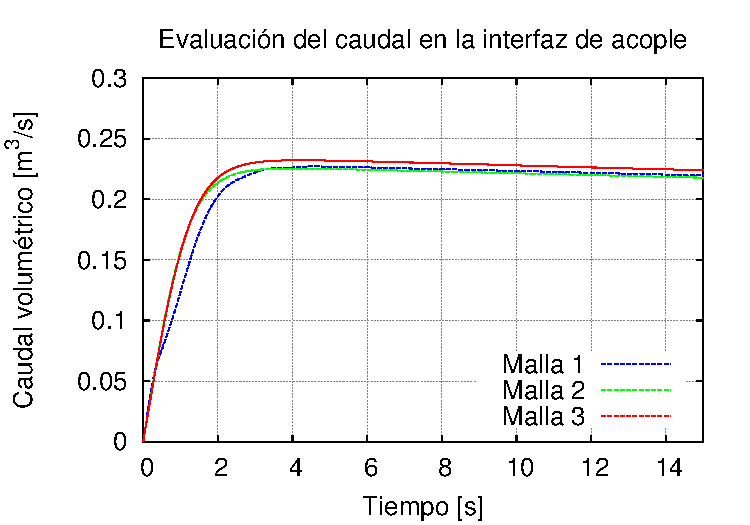
\includegraphics[scale=0.55]{q_vs_t.pdf}
		%\caption{t=250 s}
		\label{asd}	
	\end{minipage}
	\caption[Evolución de la presión y del caudal volumétrico en la interfaz de acople]
  {Evolución de la presión y del caudal volumétrico en la interfaz de acople entre los dos subsistemas.
  La presión atmosférica es de 92000 Pa.}  
	\label{qpvst}
\end{figure}

%~ \begin{figure}[ht]
%~ \centering{}\includegraphics[scale = 1]{qpvst.pdf}
%~ \caption{Evolución de la presión y del caudal volumétrico en la interfaz de acople entre los dos subsistemas.}
%~ \label{qpvst}
%~ \end{figure}

En la Figura \ref{hvst} se observa la evolución de la altura de la superficie libre del líquido en el tanque durante los primeros quince segundos obtenida en diferentes cálculos.
La curva azul reporta los resultados obtenidos con la malla más gruesa, la curva roja los resultados obtenidos con la malla intermedia y la curva violeta los resultados obtenidos con la malla más fina.
La curva verde muestra resultados de análisis estudiando la condición inicial de gas de relleno en las cañerías, que será descripta en la sección \ref{3:level-set}.
Las curvas cyan y gris muestran resultados del cálculo del modelo tri-dimensional del tanque con acoplamiento débil al modelo cero dimensional de la red hidráulica \cite{ra10-paper}.
La primera curva fue obtenida sin utilizar modelo de turbulencia, y la segunda utilizando el modelo RANS previamente comentado.
Comparativamente se muestran también los valores experimentales reportados en la referencia \cite{invap-mockup}.

\begin{figure}[ht]
\centering
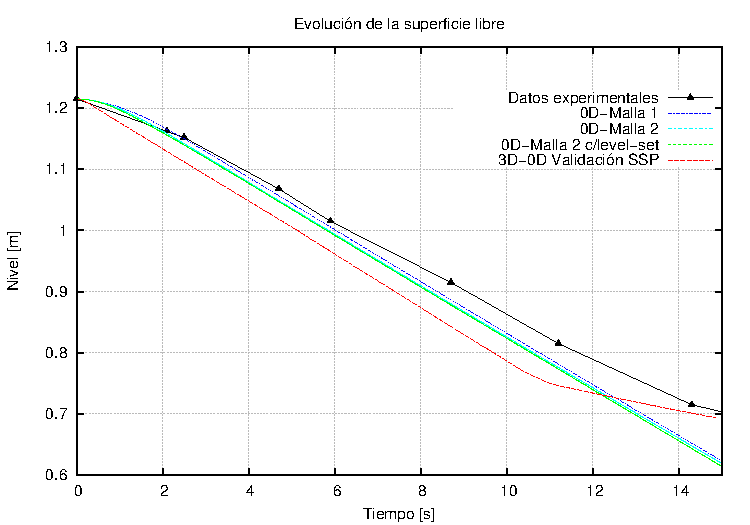
\includegraphics[scale = 1]{hvst.pdf}
\caption[Evolución del nivel de líquido en el \textit{mockup} del tanque del reflector del reactor OPAL ante accionamiento del SSP]
{Evolución del nivel de líquido en el \textit{mockup} del tanque del reflector del reactor OPAL ante accionamiento del SSP.
La curva negra está construida con datos experimentales proporcionados por INVAP S.E.
Las curvas azul, roja, verde y violeta reportan datos calculados mediante diferentes mallas para el modelo tri-dimensional del arreglo de válvulas, 
con acoplamiento fuerte al modelo cero-dimensional del resto del sistema.
Las curvas cyan y gris muestran resultados del cálculo del modelo tri-dimensional del tanque con acoplamiento débil al modelo cero dimensional de la red hidráulica.}
\label{hvst} 
\end{figure}

Los modelos computacionales predicen un comportamiento dinámico similar al reportado experimentalmente.
Durante los primeros segundos de evolución existe una cierta inercia en la descarga que solo es captada por los modelos que describen el detalle en el arreglo de válvulas.
Tras este transitorio inicial, todos los modelos predicen una pendiente de vaciado similar.
Esta pendiente se corresponde con similares caudales de descarga entre los diferentes modelos, 
con lo que se verifica que la pérdida de carga total considerada en dos modelos independientes (modelo tri-dimensional del tanque acoplado, y modelo cero-dimensional del tanque acoplado) es similar.
La curva experimental presenta ciertas ondulaciones que se deben al efecto que el oleaje en la superficie del líquido genera sobre el punto de medición.
Estas variaciones son filtradas en los modelos utilizados, 
ya que las curvas calculadas reportan alturas efectivas, computadas a partir del volumen restante de líquido en el tanque.
Transcurridos diez segundos de evolución, existe un quiebre en las curvas del modelo tri-dimensional del tanque.
Este quiebre se corresponde al momento en el que las cañerías succionan tanto gas que es posible desacoplar el modelo cero-dimensional de pérdida de carga,
basándose en la hipótesis de que se establece una vena gaseosa entre el punto de succión y el orificio de descarga.
Esta hipótesis es conservativa para el objetivo de estudio previsto,
ya que si el acoplamiento de la red no fuera realmente despreciable, el tanque se vaciaría a mayor velocidad que la modelada.
En el tanque existe un cajón que envuelve la entrada a la red hidráulica y no permite el vaciado más allá de los 60 cm,
por lo que el nivel de líquido, que es medido fuera de este cajón, tiende asintóticamente a este valor.
Esta dinámica no es considerada en el modelo cero-dimensional del tanque, lo que explica las diferencias entre las curvas en los últimos segundos.

\subsection*{Análisis de sensibilidad de resultados ante válvula en falla}

Los cálculos previos se realizaron suponiendo que falla la válvula de la última conexión entre los colectores.
Es de interés conocer si existe variación en los tiempos de descarga si la válvula que falla es alguna otra.
En la Figura \ref{hvstv} se compara la evolución de la superficie libre ante fallas en la primera, la tercera y la sexta válvula.

\begin{figure}[ht]
\centering
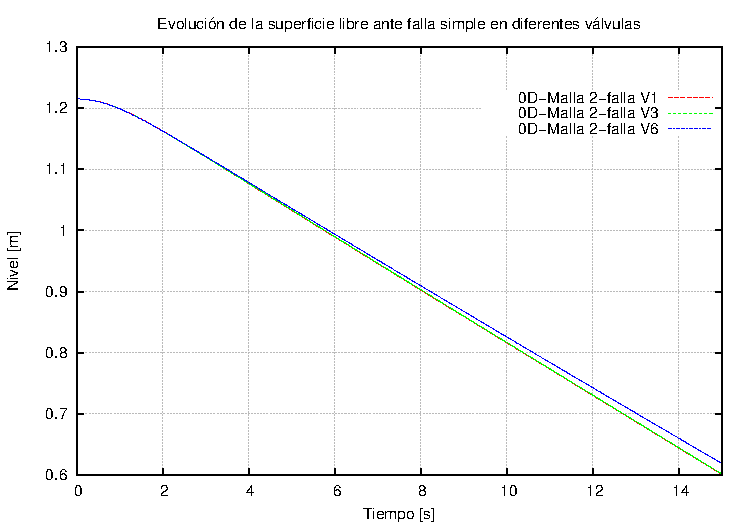
\includegraphics[scale = 1]{hvstv.pdf}
\caption[Evolución del nivel de líquido en el \textit{mockup} del tanque del reflector del OPAL ante accionamiento del SSP considerando falla simple en diferentes válvulas]
{Evolución del nivel de líquido en el \textit{mockup} del tanque del reflector del OPAL ante accionamiento del SSP considerando falla simple en diferentes válvulas.}
\label{hvstv} 
\end{figure}

Como puede observarse no es posible notar diferencias considerables en la evolución.
La pérdida de carga total del arreglo de válvulas es levemente sensible a la válvula que falla.

\subsection*{Transporte de superficie libre en las tuberías}
\label{3:level-set}

Como se comentó, en los cálculos realizados previamente no se consideró el gas de relleno en las tuberías durante los primeros instantes del drenado.
Es de interés estudiar su influencia.
Se utiliza la técnica de level-set para transportar la superficie libre \cite{level-set}.
Para ello se añade un paso fraccionado extra al sistema de ecuaciones (\ref{eq-mani}):

\begin{equation}
\left\{ \begin{array}{rcl}
\displaystyle \frac{\partial\phi}{\partial t}+ (\bar{u} \cdot \nabla) \phi &=& 0
\label{eq-ls}
\end{array} \right.
\end{equation}
donde $\phi$ es el campo que representa la distancia con signo de cada punto a la superficie libre.
Las porciones del sistema con líquido tienen $\phi$ positivo y las porciones con gas tienen $\phi$ negativo.
$\phi$ tiene valor nulo en la superficie libre.
La ecuación (\ref{eq-ls}) requiere un valor de contorno allí donde $\bar{u} \cdot \bar{n} < 0$,
y por lo tanto debe proveerse el valor del campo a la entrada de la tubería.
Esta ecuación también es resuelta mediante una formulación de elementos finitos con elementos lineales y estabilización \textit{SUPG}.
Se utiliza, además, un enriquecimiento del espacio de presiones en los elementos de la interfaz \cite{enriq}.
El campo del level set es reinicializado mediante cálculos geométricos cada 10 pasos temporales.

\begin{figure}[ht]
\centering
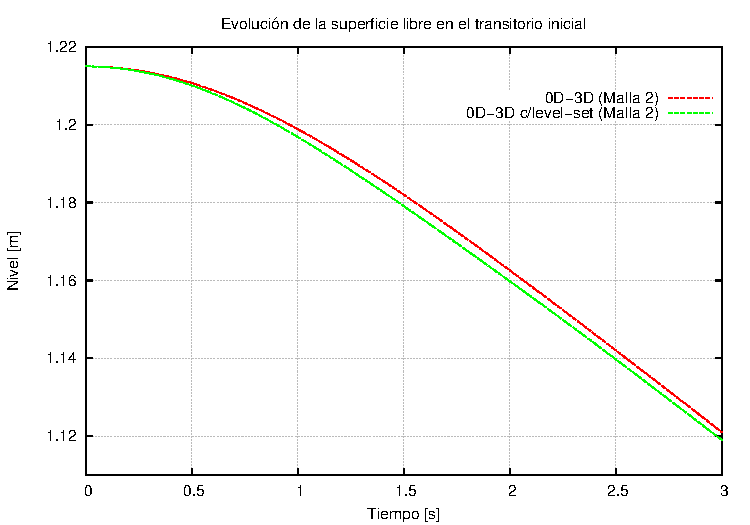
\includegraphics[scale = 1]{hvstlsZoom.pdf}
\caption[Evolución del nivel de líquido en el \textit{mockup} del tanque del reflector del reactor OPAL ante accionamiento del SSP]
{Evolución del nivel de líquido en el \textit{mockup} del tanque del reflector del reactor OPAL ante accionamiento del SSP durante el transitorio inicial.
  Se comparan la solución obtenida despreciando el gas en la cañería y la obtenida con transporte de superficie libre mediante la técnica de \textit{level-set}.}  
	\label{hvstls}
\end{figure}

En la Figura \ref{hvst} se compara la evolución obtenida de la superficie libre con los resultados anteriores,
y en la Figura \ref{hvstls} se compara la evolución durante el transitorio inicial.
Puede observarse que al modelar el transporte del gas la descarga se acelera durante el primer instante, debido a la menor pérdida de carga.
Sin embargo, este fenómeno no tiene mayor influencia.
La evolución posterior es similar a la obtenida sin el modelado de la superficie libre,
y por lo tanto la aproximación realizada inicialmente es conservativa, ya que considera una mayor pérdida de carga.

En la Figura \ref{evol-ls} se observa la evolución de la superficie libre en el arreglo de válvulas durante los primeros instantes de tiempo.

\begin{figure}[ht]
\begin{minipage}{.5\linewidth}
\centering
\subfloat[t = 0 s]{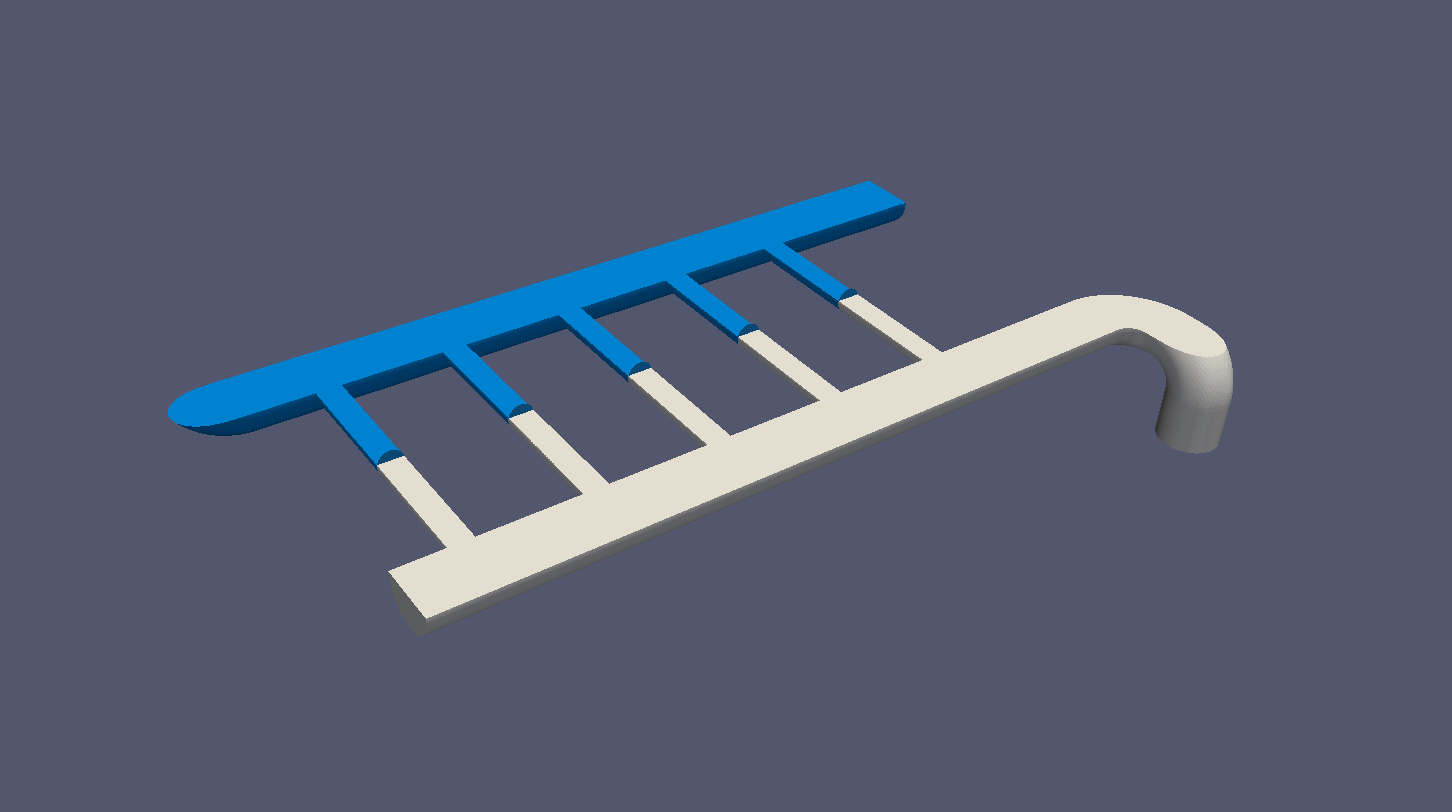
\includegraphics[scale=0.135]{0ms.png}}\\
\subfloat[t = 0.6 s]{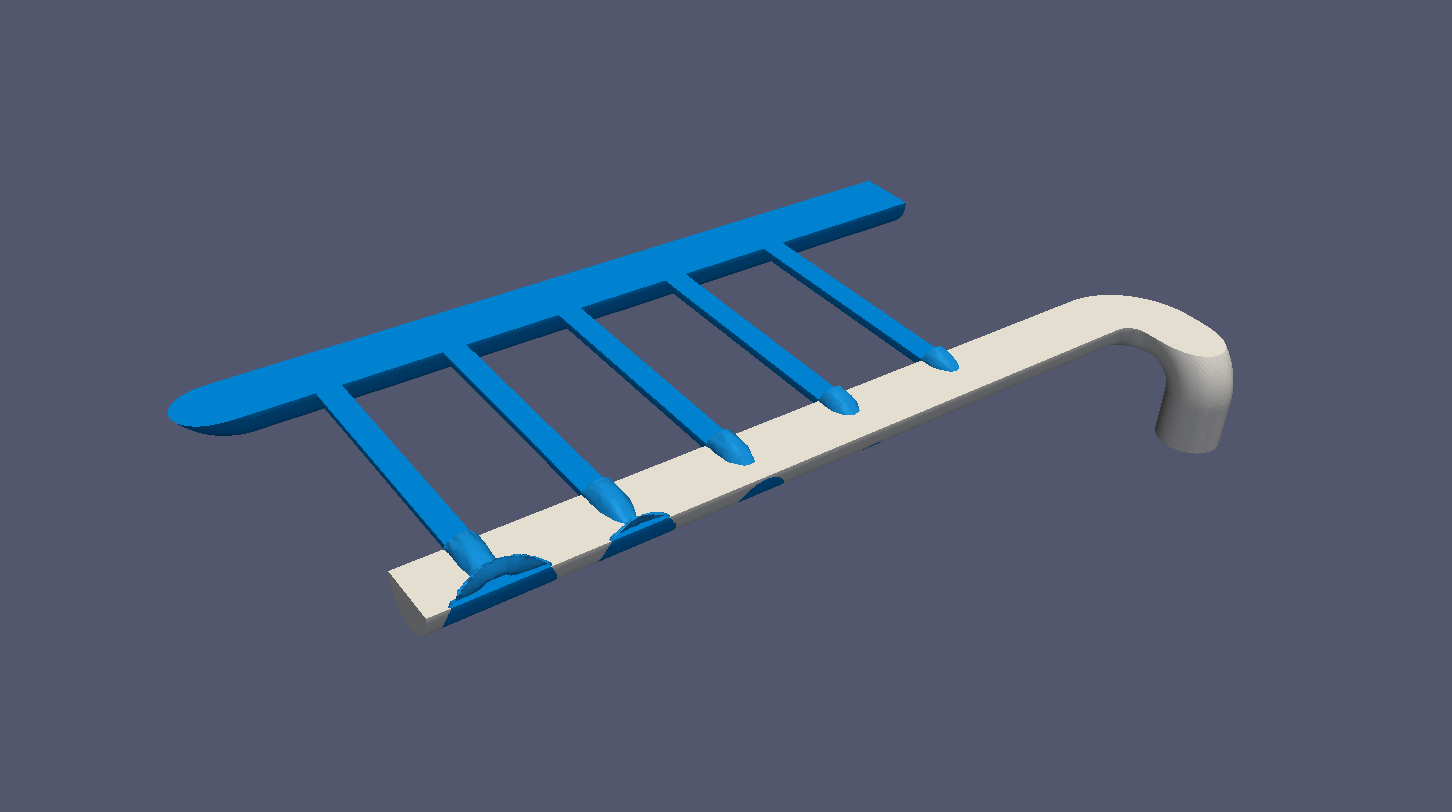
\includegraphics[scale=0.135]{600ms.png}}\\
\subfloat[t = 1.2 s]{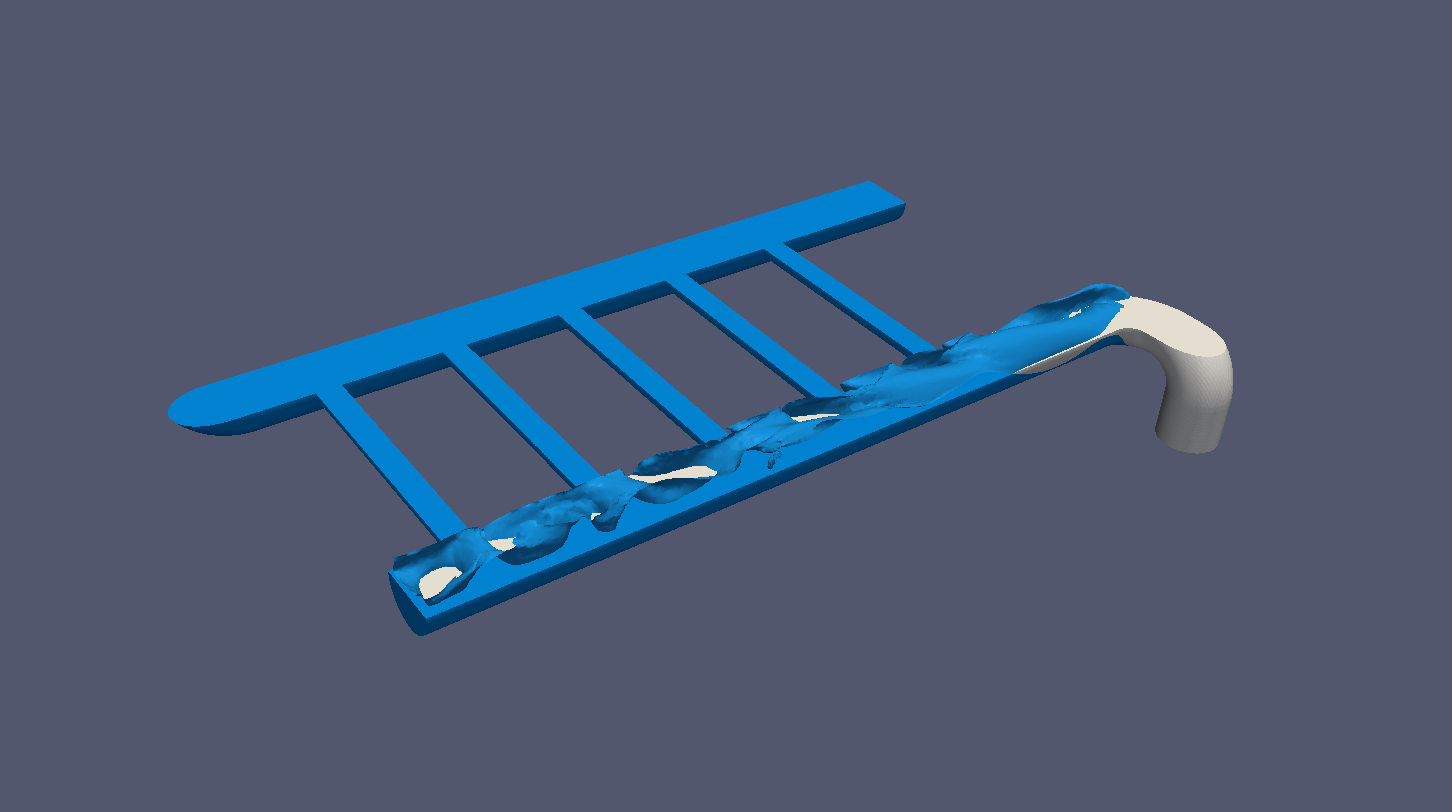
\includegraphics[scale=0.135]{1200ms.png}}
\end{minipage}\hfill
\begin{minipage}{.5\linewidth}
\centering
\subfloat[t = 0.3 s]{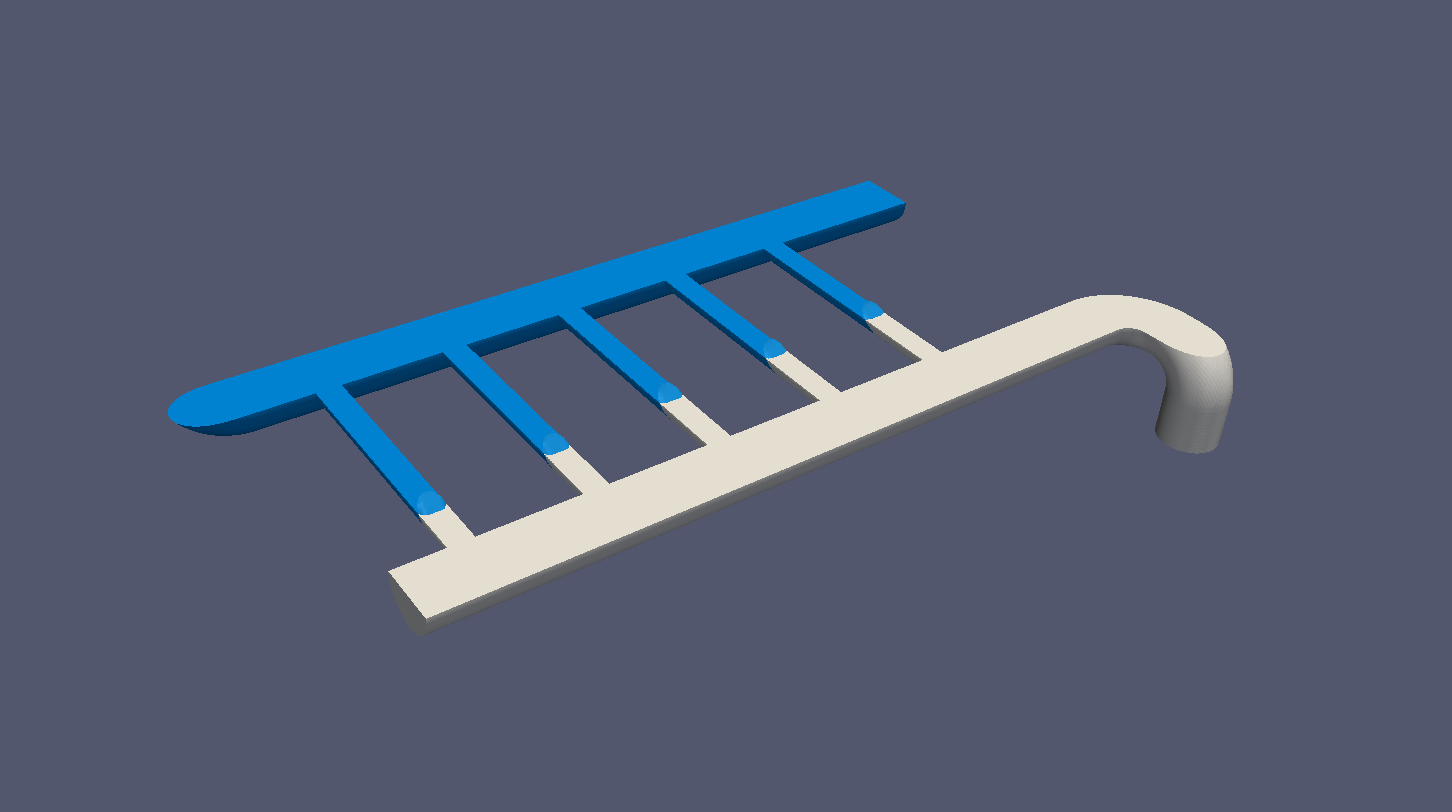
\includegraphics[scale=0.135]{300ms.png}}\\
\subfloat[t = 0.9 s]{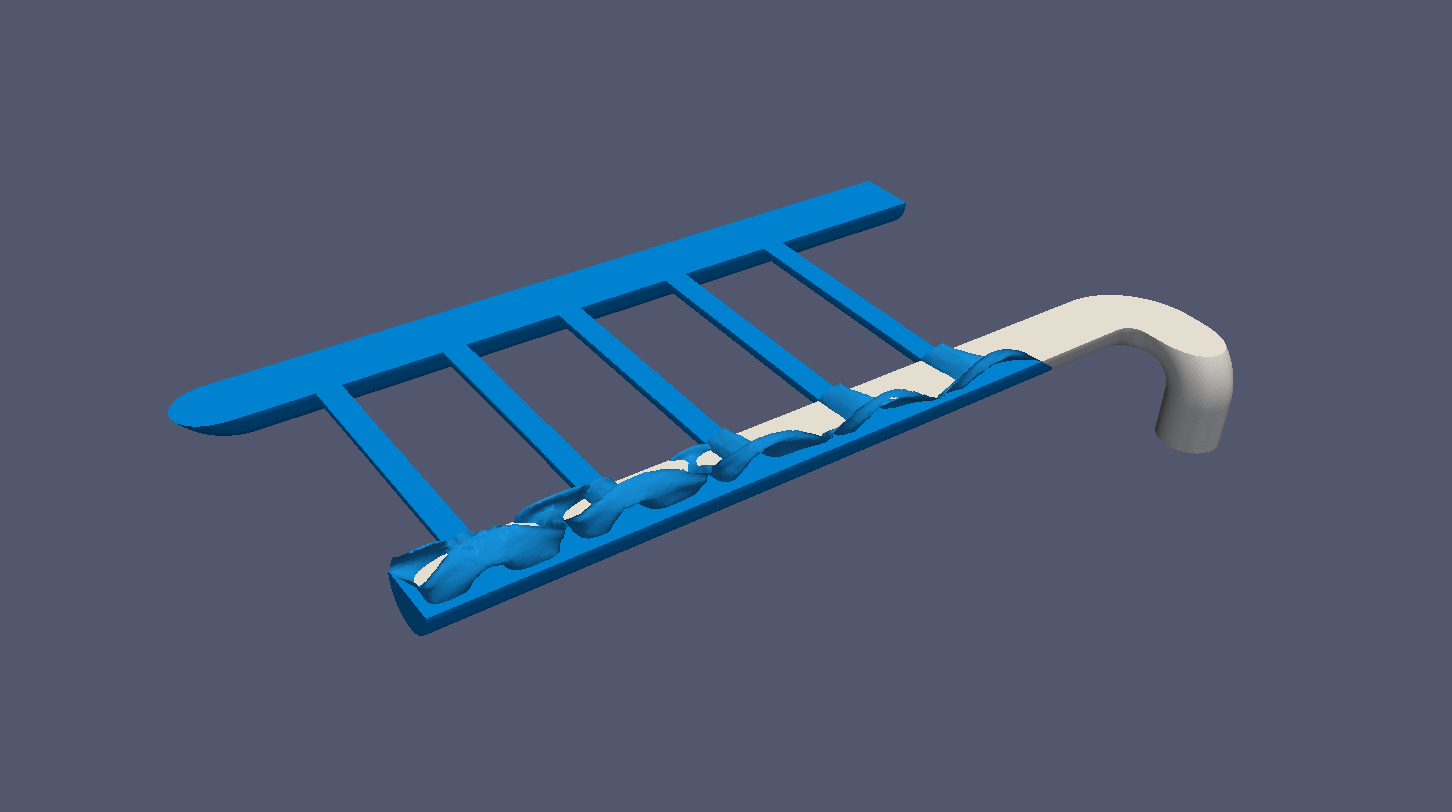
\includegraphics[scale=0.135]{900ms.png}}\\
\subfloat[t = 2.0 s]{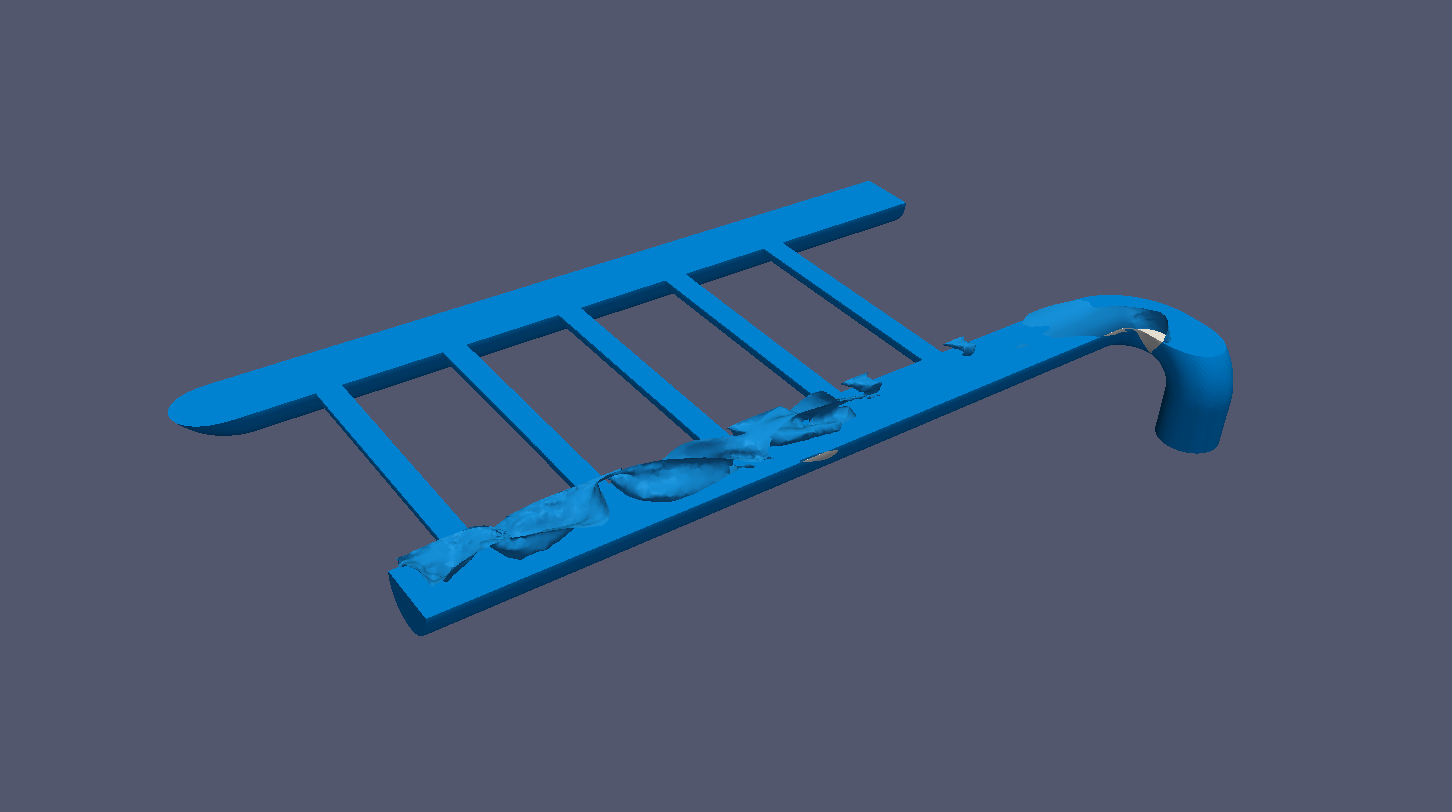
\includegraphics[scale=0.135]{2000ms.png}}
\end{minipage}
\caption[Transitorio inicial de la descarga del tanque a través del arreglo de válvulas del \textit{mockup} del reactor OPAL, con detalle de la evolución de la superficie libre]
{Transitorio inicial de la descarga del tanque a través del arreglo de válvulas, con falla simple en la última válvula
  (no se modela).
	El corte horizontal en la geometría permite observar el detalle de la evolución de la superficie libre.
  El líquido (azul) se encuentra inicialemente en condición estática rellenando las cañerías hasta la posición de las válvulas.
  Al otro lado el gas (blanco) rellena el resto de la red hidráulica.}  
\label{evol-ls}
\end{figure}

\subsection*{Conclusiones del análisis}
La herramienta de análisis de acoplamiento fuerte de subsistemas permite incorporar el estudio de la inercia fluídica en la red hidráulica de descarga.
Este estudio revela que los modelos que incluyen el fenómeno inercial del fluido en la red hidráulica del \textit{mockup} del SSP del OPAL predicen un retraso de la descarga en un máximo de un segundo 
respecto a los modelos que no lo incluyen.
Como la inclusión del efecto inercial modela una dinámica similar a la reportada experimentalmente durante el transitorio inicial y,
además, es conservativa en función del objetivo de estudio establecido, debería ser considerada en futuros análisis de seguridad.

\subsection*{Análisis de métodos de resolución del sistema de ecuaciones de residuos}

A fines de comparar la efectividad de diferentes métodos numéricos se realizaron distintos cálculos utilizando la malla más gruesa.
La Figura \ref{nonlinear_fevals} compara la cantidad de evaluaciones de funciones en función del paso temporal para diferentes métodos de resolución.

\begin{figure}[ht]
\centering
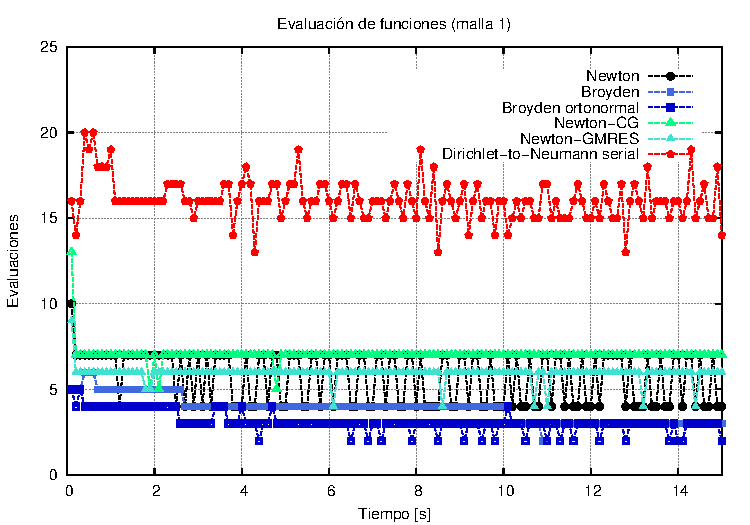
\includegraphics[scale = 1]{nonlinear_fevals.pdf}
\caption[Evaluación de diferentes métodos numéricos no lineales en el problema del vaciado del tanque reflector del \textit{mockup} del reactor OPAL]
{Evaluación de diferentes métodos numéricos en la resolución del sistema de ecuaciones de residuos resultante para el problema del vaciado del tanque reflector del \textit{mockup} del reactor OPAL.
El método explícito \textit{Dirichlet-to-Neumann} requiere excesiva cantidad de evaluaciones en cada paso de tiempo,
mientras que los métodos implícitos \textit{quasi-Newton} son los más eficientes.}
\label{nonlinear_fevals}
\end{figure}

El método explícito \textit{Dirichlet-to-Neumann} es el que mayor cantidad de evaluaciones consume, debido a que requiere una excesiva cantidad de iteraciones para converger.
Los métodos de tipo \textit{Newton-Krylov}: \textit{Newton-GMRES} y \textit{Newton-CG} (\textit{Newton-Gradientes Conjugados}) requieren baja cantidad de iteraciones, 
pero debido a la forma de resolución toman más evaluaciones que los métodos \textit{quasi-Newton}: \textit{Broyden} y \textit{Broyden ortonormal},
los cuales convergen con baja cantidad de iteraciones y de evaluaciones asociadas
(solo en el primer paso de cálculo involucran mayor cantidad de evaluaciones debido a que inicializan la matriz jacobiana por diferencias finitas).
El método de \textit{Newton-Raphson} toma tantas evaluaciones como los métodos \textit{Newton-Krylov},
sin embargo, estas evaluaciones están asociadas a muy baja cantidad de iteraciones,
ya que consume evaluaciones en la construcción de la matriz jacobiana.

En conclusión, al igual que en los resultados presentados en la sección \ref{3:mockup}, los métodos \textit{Broyden} y \textit{Broyden ortonormal} resultaron ser los más eficientes.
A fines de acelerar aún más el cálculo, se estudió la forma de optimizarlos.
Se ensayaron diferentes métodos para la propuesta de semillas del vector de incógnitas $\bar{x}_n$ y de la matriz $\mathbb{B}_n$ para cada paso temporal de resolución.
Hasta ahora las semillas para el primer paso temporal eran el vector de ceros $\bar{x}_1=\bar{0}$ y la matriz identidad $\mathbb{B}_1=\mathbb{I}$,
y las semillas para cualquier paso temporal próximo eran el vector $\bar{x}_{n-1}$ de la solución convergida en el paso previo,
y la matriz $\mathbb{B}_{n-1}$ de la última iteración correspondiente a ese paso.
Ahora el objetivo radica en intentar generar semillas que aceleren la convergencia.

Se propone utilizar un método de extrapolación, a partir de la información de los resultados que se van obteniendo en los sucesivos pasos.
La semillas para $\bar{x}_n$ y para $\mathbb{B}_n$ podrían tener órdenes de extrapolación $k_{\bar{x}}$ y $k_{\mathbb{B}}$ diferentes.
En el paso $n$, se van a utilizar los valores de los vectores $\bar{x}_i$, con $i  \in  \left \{ n-1-k_{\bar{x}}, n-1\right \}$,
y los valores de las matrices $\mathbb{B}_j$, con $j  \in  \left \{ n-1-k_{\mathbb{B}}, n-1\right \}$.
Estas extrapolaciones son válidas solo cuándo $n>k_{\bar{x}}+1$ y $n>k_{\mathbb{B}+1}$ respectivamente.

\begin{figure}[ht]
\centering
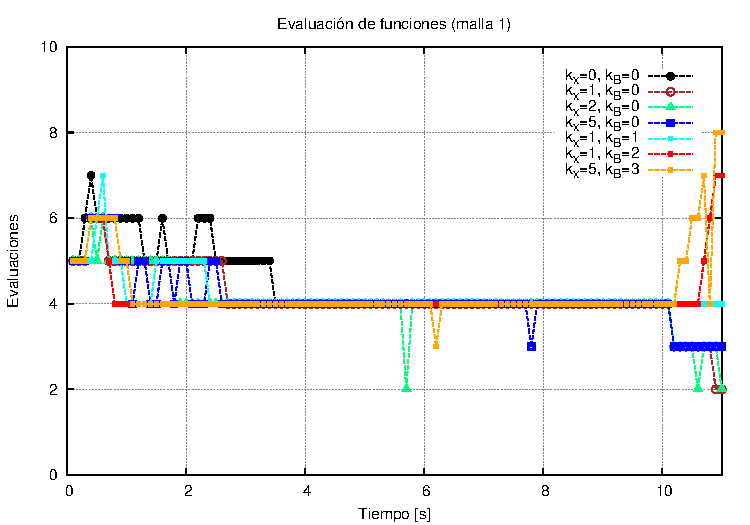
\includegraphics[scale = 1]{nonlinear_fevals_ex.pdf}
\caption[Eficiencia para diferentes esquemas de extrapolación en la generación de semillas]
{Eficiencia para diferentes esquemas de extrapolación en la generación de semillas para $\bar{x}_n$ y $\mathbb{B}_n$ en cada paso temporal.
$k_{\bar{x}}$ indica el órden de extrapolación para $\bar{x}_n$ y $k_{\mathbb{B}}$ indica el órden de extrapolación para $\mathbb{B}_n$ utilizado en cada esquema.
Los métodos con alto órden de extrapolación para $\mathbb{B}_n$ requieren menor cantidad de iteraciones para converger el cálculo en la primer etapa,
pero a su vez requieren excesivas iteraciones ante alguna perturbación en los resultados.
Los métodos con algún órden de extrapolación para $\bar{x}_n$ son más eficientes en estas instancias.}
\label{nonlinear_fevals_ex}
\end{figure}
La Figura \ref{nonlinear_fevals_ex} reporta la cantidad de evaluaciones de funciones requeridas para la convergencia en cada paso temporal,
jugando con diferentes órdenes de extrapolación para $\bar{x}_n$ y $\mathbb{B}_n$.
Las evaluaciones de funciones aquí están directamente relacionadas con las iteraciones necesarias para la convergencia,
ya que el método de \textit{Broyden} realiza una sola evaluación en cada iteración.
Al comienzo del cálculo todos los esquemas numéricos requieren excesivas iteraciones para converger,
y luego comienzan a converger con menor cantidad de iteraciones.
El cálculo con órden nulo de extrapolación para ambas variables es el que más tarda en bajar la cantidad de iteraciones.
Le siguen todos aquellos esquemas sin extrapolación para la matriz $\mathbb{B}_n$.
Los esquemas con $k_{\mathbb{B}}=3$ y $k_{\mathbb{B}}=5$ son los que más rápidamente bajan la cantidad de iteraciones,
por lo que se deduce que la extrapolación para la generación de semillas para $\mathbb{B}_n$ es altamente útil para arrancar el cálculo.
En etapas avanzadas la matriz $\mathbb{B}_n$ se estabiliza y comienza a converger a resultados similares en los sucesivos pasos.
Es decir, la tasa de cambio del vector solución $\bar{x}_n$ se vuelve aproximadamente constante (como puede observarse en la Figura \ref{qpvst}).
Ante una pequeño cambio, los esquemas de extrapolación para $\mathbb{B}_n$ amplifican esta perturbación y comienzan a generar malas semillas,
por lo que comienzan a requerir mayor cantidad de iteraciones para converger.
Este efecto puede observarse a partir de los $10s$ de cálculo.
Por el contrario, los esquemas con bajo órden de extrapolación para $\mathbb{B}_n$ y algún órden de extrapolación para $\bar{x}_n$ son más eficientes en esta etapa.
Aquí podría pensarse que los esquemas de extrapolación son inestables ante perturbaciones en $\mathbb{B}_n$, pero estables para perturbaciones en $\bar{x}_n$.

En base a estos resultados, se deduce que el esquema de generación de semillas idóneo
requiere órdenes de extrapolación $k_{\bar{x}}$ y $k_{\mathbb{B}}$ dependientes del tiempo,
comenzando con alto $k_{\mathbb{B}}$ y bajo $k_{\bar{x}}$, y tendiendo a $k_{\mathbb{B}}=0$ y alto $k_{\bar{x}}$ a medida que avanza el cálculo.

\section{Resolución de redes hidráulicas de múltiples componentes}
\label{3:redes}

\subsection*{Presentación del problema}
\label{3:redes-presentacion}

Con interés en conocer el comportamiento de la metodología de resolución
para problemas abordados mediante el Método de Descomposición Disjunta de Dominios en sistemas con grandes cantidades de incógnitas,
se propuso analizar redes hidráulicas de múltiples componentes interconectados.
La idea es utilizar modelos sencillos que describan el comportamiento de cada componente particular para poder centrar el análisis solo en el estudio de convergencia
de resultados, analizando estados estacionarios.

\subsection*{Subsistemas de estudio}
\label{3:redes-subsistemas}

Se proponen sistemas de redes hidráulicas ramificadas divergentes.
Debido a la metodología de abordaje propuesta en el trabajo, las interfaces deben seleccionarse de forma que cada una de ellas solo conecte dos subdominios contiguos.
Por lo tanto, cada porción del sistema que comprende una ramificación es pensada como un subdominio diferente,
de modo que cada subdominio contenga tres interfaces de acoplamiento.
La Figura \ref{net16} esquematiza un modelo de estudio con 5 subsistemas acoplados.
Los parámetros geométricos de cada subsistema se sortean aleatoriamente entre valores típicos.
El fluido de trabajo es agua a temperatura y presión ambiente.

\begin{figure}[ht]
\centering{}
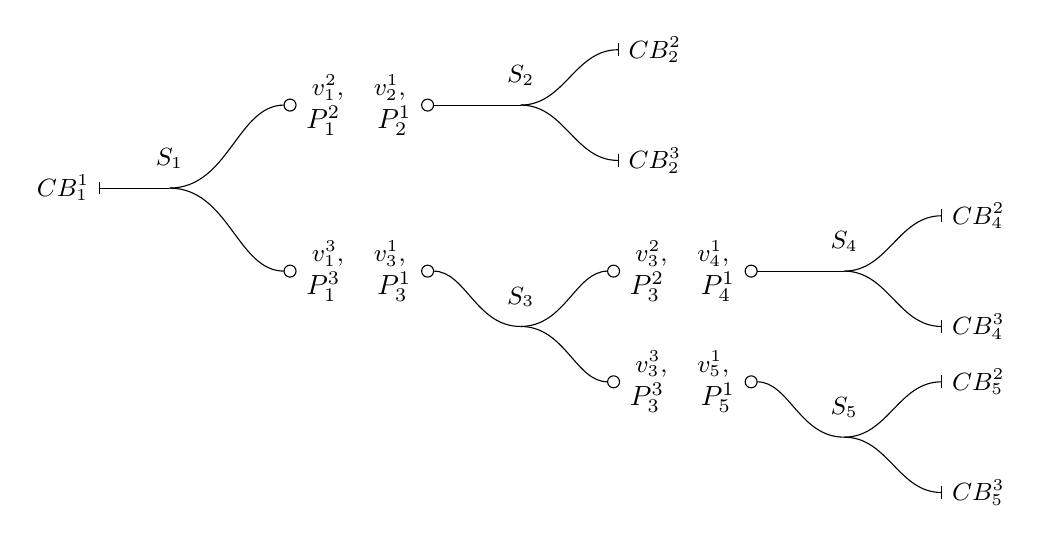
\begin{tikzpicture}

% Nodos
\node [label={\small $S_3$}] at (0em,0em) (n8) {};

\node [right of=n8, xshift=3em, yshift=-2em, align=center] (n13) {\small $v_{3}^{3}, \quad v_{5}^{1},$ \\ $P_{3}^{3}$ \quad $P_{5}^{1}$};
\node [right of=n13, xshift=3em, yshift=-2em, label={\small $S_5$}] (n14) {};
\node [right of=n14, xshift=2em, yshift=-2em] (n16) {\small $CB_{5}^{3}$};
\node [right of=n14, xshift=2em, yshift=2em] (n15) {\small $CB_{5}^{2}$};

\node [right of=n8, xshift=3em, yshift=2em, align=center] (n9) {\small $v_{3}^{2}, \quad v_{4}^{1},$ \\ $P_{3}^{2}$ \quad $P_{4}^{1}$};
\node [right of=n9, xshift=3em, yshift=0em, label={\small $S_4$}] (n10) {};
\node [right of=n10, xshift=2em, yshift=-2em] (n12) {\small $CB_{4}^{3}$};
\node [right of=n10, xshift=2em, yshift=2em] (n11) {\small $CB_{4}^{2}$};

\node [left of=n8, xshift=-3em, yshift=2em, align=center] (n7) {\small $v_{1}^{3}, \quad v_{3}^{1},$ \\ $P_{1}^{3}$ \quad $P_{3}^{1}$};
\node [left of=n7, xshift=-4em, yshift=3em, label={\small $S_1$}] (n2) {};
\node [left of=n2, xshift=-1em, yshift=-0em] (n1) {\small $CB_{1}^{1}$};

\node [right of=n2, xshift=4em, yshift=3em, align=center] (n3) {\small $v_{1}^{2}, \quad v_{2}^{1},$ \\ $P_{1}^{2}$ \quad $P_{2}^{1}$};
\node [right of=n3, xshift=3em, yshift=0em, label={\small $S_2$}] (n4) {};
\node [right of=n4, xshift=2em, yshift=2em] (n5) {\small $CB_{2}^{2}$};
\node [right of=n4, xshift=2em, yshift=-2em] (n6) {\small $CB_{2}^{3}$};

% Conexiones
\draw[|-] (n1.east) to [in=180, out=0] (n2.center);
\draw[-o] (n2.center) to[in=180, out=0] (n3.west);
\draw[-o] (n2.center) to[in=180, out=0] (n7.west);

\draw[o-] (n3.east) to[in=180, out=0] (n4.center);
\draw[-|] (n4.center) to[in=180, out=0] (n5.west);
\draw[-|] (n4.center) to[in=180, out=0] (n6.west);

\draw[o-] (n7.east) to[in=180, out=0] (n8.center);
\draw[-o] (n8.center) to[in=180, out=0] (n9.west);
\draw[-o] (n8.center) to[in=180, out=0] (n13.west);

\draw[o-] (n9.east) to[in=180, out=0] (n10.center);
\draw[-|] (n10.center) to[in=180, out=0] (n11.west);
\draw[-|] (n10.center) to[in=180, out=0] (n12.west);

\draw[o-] (n13.east) to[in=180, out=0] (n14.center);
\draw[-|] (n14.center) to[in=180, out=0] (n15.west);
\draw[-|] (n14.center) to[in=180, out=0] (n16.west);

\end{tikzpicture}
\caption[Descomposición disjunta de dominios en el modelado de redes hidráulicas]
{Descomposición disjunta de dominios en un modelo de red hidráulica con 16 incógnitas en las interfaces de acoplamiento.
La incógnita $v_{i}^{j}$ refiere a la velocidad media en el extremo $j$ del subsistema $i$.
La incógnita $P_{i}^{j}$ agrupa las presiones estática y dinámica medias en el extremo $j$ del subsistema $i$.
Las incógnitas pueden reducirse rápidamente a la mitad aplicando relaciones de continuidad de campos de variables.}
\label{net16}
\end{figure}

Cada subdominio es modelado con balances cero-dimensionales de conservación de masa y energía.
Las ecuaciones resultantes para un subsistema genérico que no contiene bordes del dominio original son las siguientes:
\begin{equation}
\left \{
\begin{array}{rcl}
\frac{p_1}{\rho} + \frac{{v_1}^2}{2} &=& \frac{p_2}{\rho} + \frac{{v_2}^2}{2} + gz_2 + \Delta u_{12} \\
\frac{p_1}{\rho} + \frac{{v_1}^2}{2} &=& \frac{p_3}{\rho} + \frac{{v_3}^2}{2} + gz_3 + \Delta u_{13} \\
A_1 v_1 &=& A_2 v_2 + A_3 v_3
\end{array}
\right .
\label{net-eq}
\end{equation}
donde los subíndices $1$, $2$ y $3$ refieren a diferentes extremos locales del contorno del subdominio,
$p_i$, $v_i$, $z_i$, y $A_i$ indican \textit{presión}, \textit{velocidad}, \textit{altura} y \textit{área} de la sección en el extremo $i$ respectivamente,
y $\Delta u_{ij}$ refiere a la diferencia de energía del flujo entre los exremos $i$ y $j$.
El extremo 1 siempre corresponde al izquierdo de cada subdominio, y las otros se numeran en forma horaria creciente.
Deben prestarse algunas consideraciones extras en las ecuaciones para los subsistemas que requieren condiciones $CB_{k}^{l}$ sobre extremos que pertenecían al borde original del sistema completo,
donde $k$ indica el subsistema y $l$ el extremo local.

Los términos de presión estática $\frac{p_i}{\rho}$ y presión dinámica $\frac{{v_i}^2}{2}$ para el extremo $i$ pueden agruparse en una única incógnita $P_i$ para simplificar el cálculo:

\begin{equation}
P_i = \frac{p_i}{\rho} + \frac{{v_i}^2}{2}
\label{p-eyd}
\end{equation}

El término $\Delta u_{ij}$ puede aproximarse mediante una función de pérdida de carga como \cite{white}:
\begin{equation}
\Delta u_{ij} = \frac{{v_i}^2}{2} \left ( \frac{f_{D_i} L_{i}}{D_i} + \sum_t K_{i,t} \right ) + \frac{{v_j}^2}{2} \left ( \frac{f_{D_j} L_{j}}{D_j} + \sum_t K_{j,t} \right )
\label{du}
\end{equation}
En esta ecuación, el primer término está modelando la pérdida de carga total entre el extremo $i$ y el nodo de divergencia,
y el segundo extremo modela la pérdida de carga total entre este nodo y el extremo $j$.
Las variables $D_i$ y $L_i$ corresponden al \textit{diámetro} y a la \textit{longitud} de la cañería desde el extremo $i$ hasta el nodo de divergencia,
$f_{D_i}$ corresponde al \textit{factor de Darcy} del flujo en esa porción
y $K_{i,t}$ corresponde al \textit{factor de pérdida de carga concentrada t} de cualquier componente hidráulico presente lo largo de algún punto de esa porción de cañería.
Bajo algunas modificaciones sería posible incorporar cambios en las secciones a lo largo de estas porciones, pero no se realizó por simplicidad.

Considerando que el flujo corre por la red hidráulica en régimen laminar, el \textit{factor de Darcy} $f_{D_i}$ puede modelarse como \cite{white}:
\begin{equation}
f_{D_{{i},lam}} = \frac{64}{Re_{D_i}}
\label{f-lam}
\end{equation}
donde $Re_{D_i}=\frac{\rho v_i D_i} {\mu_i}$, siendo $\mu$ la viscocidad dinámica del fluido.
Bajo esta aproximación, la ecuación \ref{du} queda lineal en $v_i$ y en $v_j$ para aquellos subsistemas en los que pudiera despreciarse la pérdida de carga concentrada:
\begin{equation}
\Delta u_{ij,lam} = \frac{{v_i}}{2} \left ( \frac{64 \mu L_{i}}{\rho {D_i}^{2}} \right ) + \frac{{v_j}}{2} \left ( \frac{64 \mu L_{j}}{\rho {D_j}^{2}} \right )
\label{du}
\end{equation}


\subsection*{Estrategia de resolución}
\label{resolucion-net}

Conforme al esquema de resolución descripto en la sección \ref{1:abordaje},
es necesario definir una estrategia para las condiciones de borde en las interfaces de acoplamiento de cada subsistema.
La estrategia propuesta es establecer condiciones de tipo \textit{Dirichlet} sobre las interfaces ubicadas a la izquierda de cada subdominio (fijando $v$)
y condiciones de tipo \textit{Neumann} sobre las interfaces ubicadas a la derecha (fijando $P$).
Considerando las ecuaciones de continuidad \ref{continuidad} se seleccionan una serie de ecuaciones modelos \ref{ecuaciones-modelos}
a partir de las relaciones \ref{net-eq} de manera que cada subproblema quede bien planteado.
En cada interfaz de acoplamiento de cada subsistema queda definida una ecuación de residuo:

\begin{equation}
\left \{
\begin{array}{rcl}
R_1 &=& v_1^{2,guess} - v_1^{2,calc} \\
R_2 &=& v_1^{3,guess} - v_1^{3,calc} \\
R_4 &=& P_2^{1,guess} - P_2^{1,calc} \\
...
\end{array}
\right .
\end{equation}
donde la cantidad de residuos depende del tamaño del sistema a analizar.

Las ecuaciones de cada subsistema son resueltas mediante funciones escritas en \texttt{Octave}.
En este caso el acoplamiento de funciones se da a través de una función \textit{maestra} también escrita en \texttt{Octave}.

\subsection*{Redes hidráulicas con regímenes de flujo laminar}
\label{laminar}

En la Figura \ref{net_linear} (a) se pueden observar la cantidad de iteraciones requeridas por diferentes métodos para la convergencia de resultados
en sistemas hidráulicos laminares sin pérdidas de carga concentrada,
variando la cantidad de subsistemas acoplados.
La cantidad de incógnitas en el eje $x$ corresponde a la simplificación obtenida tras aplicar las ecuaciones de continuidad \ref{continuidad}.

\begin{figure}[ht]
	\begin{minipage}{0.5\linewidth}
		\centering
		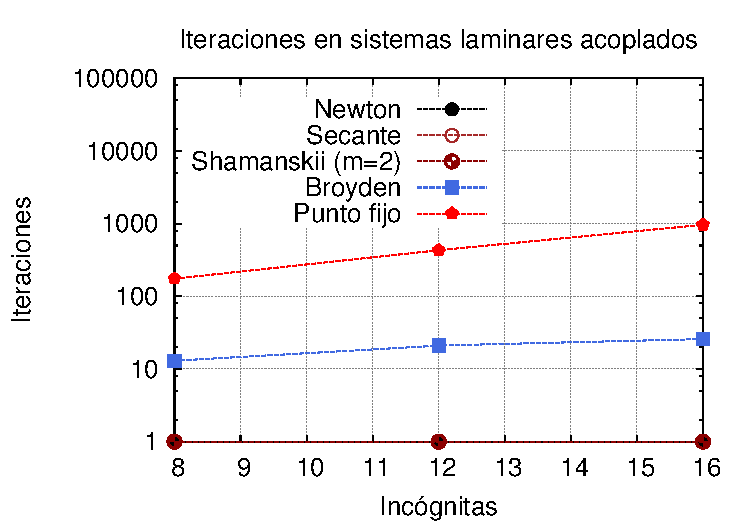
\includegraphics[scale=0.55]{net_linear_its.pdf}
	\end{minipage}
	\begin{minipage}{0.5\linewidth}
		\centering
		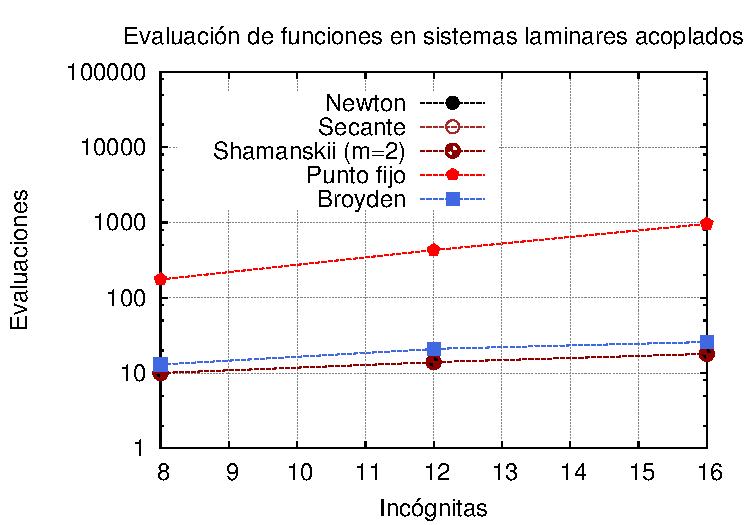
\includegraphics[scale=0.55]{net_linear_fevals.pdf}
	\end{minipage}
	\caption[Comparación de diferentes métodos numéricos para la resolución de sistemas de redes hidráulicas]
  {Comparación de diferentes métodos numéricos para la resolución de sistemas de redes hidráulicas:
  (a) iteraciones requeridas y (b) evaluaciones de funciones requeridas.}
  \label{net_linear}
\end{figure}

En la figura se observa que el método del punto fijo requiere excesiva cantidad de iteraciones.
Las mismas ascienden hasta 1000 para sistemas con 16 incógnitas reducidas,
pero este valor puede variar dependiendo de las semillas iniciales y de los parámetros del sistema.
El método de \textit{Broyden} requiere decenas de iteraciones para cada sistema.
El método de \textit{Newton-Raphson}, el método de la \textit{secante}
y el método de \textit{Shamanskii} de tipo $m$=2
requieren solo una iteración, debido a que los sistemas de cálculo son lineales
(las tres curvas se encuentran superpuestas).
Sin embargo, el parámetro de comparación de interés es la cantidad total de evaluaciones que requiere cada método.
En la Figura \ref{net_linear} (b) se observa que la ventaja obtenida por los métodos que construyen la matriz jacobiana es despreciable frente al método de \textit{Broyden}.

Debido a que los métodos \textit{quasi-Newton} han presentado elevada confiabilidad en la resolución de sistemas acoplados a lo largo de todo el trabajo,
se investigaron formulaciones alternativas al método de \textit{Broyden},
y en la Figura \ref{net_linear_its_broy} se reportan los resultados.

\begin{figure}[ht]
\centering
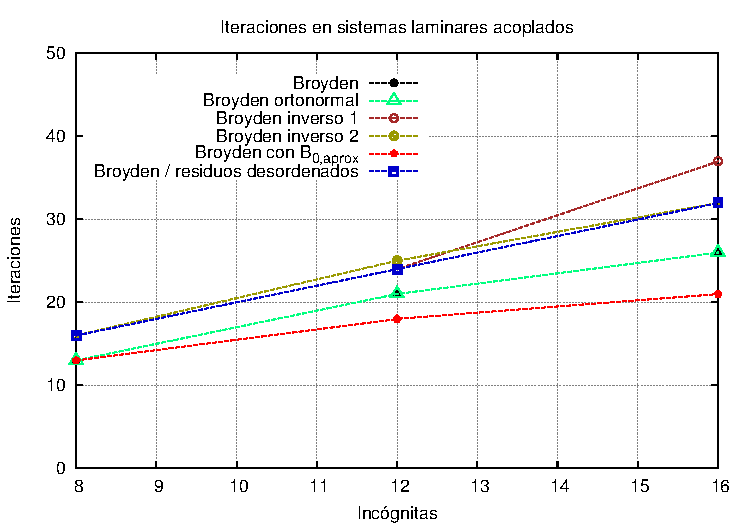
\includegraphics[scale = 1]{net_linear_its_broy.pdf}
\caption[Comparación de diferentes esquemas de \textit{Broyden} para la resolución de sistemas de redes hidráulicas con regímenes de flujo laminar]
{Comparación de diferentes esquemas de \textit{Broyden} para la resolución de sistemas de redes hidráulicas con regímenes de flujo laminar.}
	\label{net_linear_its_broy}
\end{figure}

Además del método \textit{Broyden ortonormal}, que en este estudio se comporta con igual eficiencia que el método de \textit{Broyden} (ambas curvas se solapan),
existen formulaciones que aproximan directamente la inversa de la matriz jacobiana (\textit{Broyden inverso 1} y \textit{Broyden inverso 2}).
Estos métodos se conocen en la bibliografía como \textit{bad Broyden update} (mala actualización de Broyden) \cite{griewank} y en la figura puede verse que tienen eficiencia inferior.

El método de \textit{Broyden} se utilizó también mejorando la semilla inicial para la matriz $\mathbb{B}_n$.
En los otros esquemas reportados se utiliza la matriz identidad,
pero aquí se reemplazó por una matriz con \textit{unos} en los elementos que corresponden a posiciones llenas de la matriz jacobiana original,
y \textit{ceros} en el resto de los elementos.
Este llenado es sencillo de implementar ya que simplemente depende de las relaciones de dependecia de las residuos y las incógnitas, que \textit{a priori} son conocidas.
Con esta implementación puede observarse en la curva de \textit{Broyden} con $\mathbb{B}_{0,aprox}$ que la convergencia mejora a medida que la cantidad de incógnitas aumenta.
Una mejor semilla para la matriz $\mathbb{B}_{0}$ hubiera podido generarse con un cálculo de diferencias finitas,
similar al que se venía utilizando para inicializar las matrices en las aplicaciones analizadas en \ref{3:ff} y \ref{3:mockup}.
En este caso los resultados hubieran coincidido con los resultados del método de la secante, que efectúa el cálculo aproximado de $\mathbb{J}$ y luego converge en una sola iteración.

Comúnmente las incógnitas tienen una numeración global, conforme al orden en el que se construyen las columnas de la matriz jacobiana
(cada columna representa la derivada del vector residuo respecto de alguna incógnita).
De ser posible, los residuos suelen ordenarse de forma tal que el residuo $i$ compute la diferencia entre el valor calculado y el valor \textit{guess} para la incógnita $i$.
En estos casos utilizar la matriz identidada como semilla para $\mathbb{B}_{0}$ es una buena propuesta.
La curva \textit{Broyden / residuos desordenados} corresponde a un esquema en el que el residuo $i$ se corresponde con alguna incógnita $j$ distinta de $i$.
Utilizar la matriz identidad como semilla para $\mathbb{B}_n$ es una mala propuesta en este caso,
ya que para cada fila $i$, el \textit{uno} debería ubicarse en la posición $j$.
Esto genera mayor dificultad para la convergencia.
Por lo tanto puede comprenderse que la diferencia entre las curvas \textit{azul} y \textit{roja} (que representan los resultados para el mismo método de \textit{Broyden})
depende exclusivamente de una elección inteligente en la forma de proponer la semilla para la matriz $\mathbb{B}_n$.
Esta diferencia asciende a 10 iteraciones en un sistema con 16 incógnitas reducidas.

\subsection*{Redes hidráulicas con regímenes de flujo turbulento}
\label{turbulent}

Habiendo investigado sistemas de redes hidráulicas con regímenes de flujo laminar,
el siguiente paso de estudio consiste en analizar sistemas de redes hidráulicas con regímenes de flujo turbulento.
En estos modelos se utiliza directamente la ecuación \ref{du} para representar la pérdida de carga entre dos extremos de un dado subdominio,
por lo que el sistema de ecuaciones global ahora es un sistema de ecuaciones no lineales.
Aquí los métodos estudiados en el apartado anterior se comportan de forma diferente.
El método de \textit{Newton-Raphson} ya no converge en una única iteración como lo hace en sistemas lineales.
La Figura \ref{net_nonLinear_fevals} detalla la cantidad de evaluaciones de funciones requerida por distintos métodos
para la convergencia de los resultados en sistemas con diferente cantidad de incógnitas reducidas.

\begin{figure}[ht]
\centering
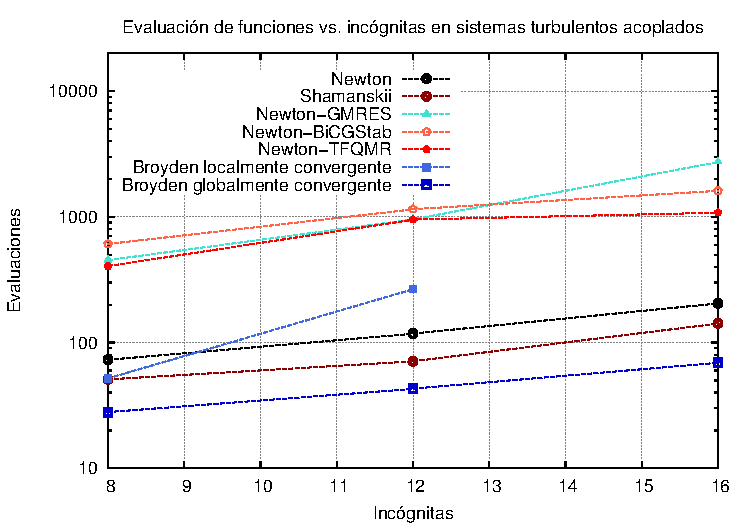
\includegraphics[scale = 1]{net_nonLinear_fevals.pdf}
\caption[Comparación de diferentes métodos numéricos para la resolución de sistemas de redes hidráulicas con regímenes de flujo turbulento]
{Comparación de diferentes métodos numéricos para la resolución de sistemas de redes hidráulicas con regímenes de flujo turbulento.}  
\label{net_nonLinear_fevals}
\end{figure}

El método explícito del punto fijo diverge en todos los sitemas analizados y por lo tanto no aparece en la gráfica.
Los métodos implícitos estudiados incluyen \textit{line searching}.
Los métodos \textit{Newton-Krylov} toman demasiadas evaluaciones para converger.
Los métodos de \textit{Newton-Raphson} y \textit{Shamanskii} tienen buena convergencia.
De estos dos el último presenta mayor ventaja ya que elude el cálculo de la matriz jacobiana en iteraciones contiguas.
El método que mejor se comporta es el método de \textit{Broyden} (globalmente convergente).
El método de \textit{Broyden local}, el único que no incluye \textit{line searching},
solo se comporta bien a baja cantidad de incógnitas, y cuando la cantidad de incógnitas es elevada diverge.

\section{Extensión a problemas acoplados en modelos de núcleo}
\label{3:extension-nucleo}

\subsection*{Estrategia de acoplamiento extendida}
\label{3:strategy-extended}

Si bien la estrategia de resolución presentada en el \hyperlink{chapter.2}{Capítulo 2}
corresponde a un equema para resolver problemas que han sido formulados mediante el Método de Descomposición Disjunta de Dominios,
el sistema de ecuaciones acoplado a resolver podría provenir de otras formulaciones,
y también ser abordados mediante la misma estrategia.
Es decir, la herramienta de acoplamiento puede ser utilizada para resolver cualquier tipo de sistemas de ecuaciones acopladas,
siempre que existan diferentes códigos que se encarguen de resolver parcialmente algunas de ellas.

A continuación se propone un modelo simplificado para el análisis de la dinámica de núcleo de un reactor nuclear.
En los dos últimos apartados se presentan ejemplos de acoplamiento neutrónico-termohidráulico utilizando este modelo.

\subsection*{Presentación del problema}
\label{3:neut-th}

La distribución espacial de la potencia generada en el núcleo de un reactor nuclear
depende de diversos factores, como la posición de barras de control, combustibles y demás materiales,
y de parámetros físicos como la temperatura del combustible, la temperatura del refrigerante o la fracción de vacío.
Los modelos neutrónicos que se utilizan para capturar esta dependencia modelan todos estos factores simplemente a través de una disposición espacial de secciones eficaces.
La distribución espacial de potencia, a su vez, genera modificaciones sobre las secciones eficaces,
ya sea debido a que está actuando como una fuente de energía, modificando temperaturas y densidades de combustibles, refrigerantes y demás materiales,
o debido al movimiento futuro requerido de materiales,
como por ejemplo, movimiento de barras de control necesarios para buscar perfiles de potencia planos, o recambio de combustibles por pérdida de criticidad.
Además, en la evolución temporal, el quemado de combustible genera alteraciones en la concentración de elementos existentes y aparición de nuevos elementos,
que también modifican las secciones eficaces.

La dinámica del núcleo de un reactor nuclear acopla fuertemente múltiples fenómenos, y cualquier modelo que se utilice para estudiarla debe abordar el acoplamiento mediante alguna estrategia.
En general, los códigos de cálculo utilizados en el área nuclear están validados para resolver solo alguno de estos fenómenos,
por lo que suele requerirse un acoplamiento entre ellos para resolver la dinámica completa.
Comúnmente este acoplamiento se resuelve mediante iteraciones explícitas de tipo \textit{Picard} dentro de cada paso de tiempo.

En esta sección se propone un modelo simplificado para el análisis de la dinámica de núcleo de un reactor nuclear durante un ciclo de quemado de elementos combustibles,
considerando solo los fenómenos neutrónico y termohidráulico.

\subsection*{Subsistemas de estudio}
\label{3:subsistemas-nt}

El cálculo de núcleo se efectúa mediante un modelo de difusión estacionario
\footnote{Al modelar un flujo neutrónico estacionario en realidad se está calculando el flujo en un reactor crítico asociado,
por lo que la distribución de potencia hallada solo es válida si el $k_{eff}$ calculado es igual a 1.
En caso contrario, debe repetirse el cálculo considerando otra distribución de secciones eficaces
(por ejemplo, moviendo barras de control).
} \cite{henry}:

\begin{equation}
\Delta \bar{\phi} = \frac{1}{k_{eff}}\Sigma \bar{\phi}
\label{eq-nucleo}
\end{equation}
donde $\bar{\phi}$ es una función vectorial con el valor del flujo neutrónico en cada punto del espacio para diferentes grupos de energía,
$\Sigma$ es la matriz de secciones eficaces asociada a diferentes reacciones para diferentes grupos de energía,
y $k_{eff}$ es el factor de multiplicación del reactor.
En el modelo propuesto las secciones eficaces dependen de la densidad del refrigerante $N_{ref}$, de la temperatura del refrigerante $T_{ref}$, de la temperatura del combustible $T_{comb}$, 
y del valor histórico de quemado $B$ del material \cite{lamarsh},
para cada punto espacial y cada grupo de energía, de modo que:

\begin{equation}
\Sigma = \Sigma \left ( N_{ref}, T_{ref}, T_{comb} \right )
\label{eq-sigma}
\end{equation}

La ecuación \ref{eq-nucleo} requiere condiciones de borde en el contorno del dominio de cálculo.
En el primer ejemplo analizado se utilizan condiciones de borde homogéneas\footnote{
Imponer un flujo $\bar{phi}$ nulo en el contorno del dominio implica utilizar la hipótesis de que el flujo se hace nulo a alguna distancia del borde (en la \textit{distancia extrapolada} \cite{lamarsh}),
y asumir al mismo tiempo que esta distancia es despreciable, para de esta forma no extender el dominio de cálculo.
} sobre $\phi$.
En el segundo ejemplo analizado se imponen condiciones de flujo entrante nulo.
Éstas se modelan mediante un artificio de absorción total de los neutrones salientes, extendiendo la malla del cálculo.

Una vez obtenido el flujo neutrónico $\phi$,
la distribución de potencia $P$ puede calcularse a partir del ritmo de reacciones de fisión \cite{lamarsh}:

\begin{equation}
P = \int_{vol} E_{fis,i} \Sigma_{fis,i} \phi_{i}
\label{power}
\end{equation}
donde $E_{fis,i}$ es la energía liberada por fisiones ocurridas en el rango de energía $i$,
$\Sigma_{fis,i}$ es la sección eficaz de fisión condensada en el grupo de energía $i$ y
$\phi_{i}$ es la componente del flujo neutrónico también dondensada en el grupo de energía $i$.
La distribución de potencia ${P}$ hallada es utilizada como fuente de energía en los cálculos acoplados de transferencia de energía.

Los fenómenos hidrodinámicos y de transferencia de calor se modelan con ecuaciones uni-dimensionales y transitorias.
La transferencia de calor a través de las estructuras de combustibles se modela con la siguiente ecuación diferencial:

\begin{equation}
\rho \frac{\partial T_{comb}}{\partial t} = \nabla \left ( k \nabla T \right )  + S
\label{relap-calor}
\end{equation}
donde $\rho$ es la densidad del medio difusivo,
$T_{comb}$ es la temperatura del combustible,
$k$ es el coeficiente de conductividad térmica y
$S$ es la fuente interna de energía.
Este último término es el que tiene la información de la distribución de potencia generada en el núcleo del reactor.
El modelo se completa con condiciones de borde adecuadas.
El refrigerante fluye alrededor de las estructuras con temperatura media $T_{sk}$ y la energía transferida entre ambos se da por convección:

\begin{equation}
-k \frac{\partial T_{comb}}{\partial n} = h \left ( T - T_{sk} \right )
\label{relap-conveccion}
\end{equation}
donde $h$ es el coeficiente de transferencia de calor que debe obtenerse a partir de algún modelo adecuado para el régimen de flujo,
y $n$ es la dirección normal al borde del dominio de cálculo de $T_{comb}$.

El modelo hidrodinámico del comportamiento del refrigerante considera una mezcla del fluido en fases líquida y gaseosa.
Las ecuaciones básicas diferenciales de este modelo son seis \cite{manual-relap-modelos}.
Las primeras dos son las ecuaciones de continuidad en cada fase:

\begin{equation}
\left \{
\begin{array}{r}
\frac{\partial} {\partial t} \alpha_g \rho_g + \frac{1}{A} \frac{\partial}{\partial x} \left (\alpha_g \rho_g v_g A \right ) = \Gamma_g \\
\frac{\partial} {\partial t} \alpha_f \rho_f + \frac{1}{A} \frac{\partial}{\partial x} \left (\alpha_f \rho_f v_f A \right ) = \Gamma_f
\end{array}
\right .
\label{relap-masa}
\end{equation}
donde los subíndices $g$ y $f$ refieren a las fases gaseosa y líquida respectivamente,
$x$ es la dirección del flujo, normal a la sección de área $A$,
$\alpha_i$ refiere a la fracción parcial de área que la fase $i$ ocupa en $A$,
$\rho_i$ es la densidad del fluido en la fase $i$,
$v_i$ es la velocidad en la dirección $x$ del fluido en la fase $i$, promediada en la sección y
$\Gamma_i$ es un término de producción fluídica en la fase $i$.
Notar que este por continuidad, $\Gamma_g = -\Gamma_f$.

Las siguientes dos ecuaciones son las ecuaciones de momento de cada fase:

\begin{equation}
\left \{
\begin{array}{r}
\alpha_g \rho_g A \frac{\partial v_g}{\partial t} + \frac{1}{2} \alpha_g \rho_g A \frac{\partial v_g^2}{\partial x} = 
- \alpha_g A \frac{\partial P}{\partial x} + \alpha_g \rho_g B_x A - \left( \alpha_g \rho_g A \right) FWG \left (v_g \right) \\
+ \Gamma_g A \left( v_{gI} - v_g \right ) - \left ( \alpha_g \rho_g A \right ) FIG \left( v_g - v_f \right) \\
-C\alpha_g\alpha_f\rho_mA \left [ \frac{\partial \left( v_g - v_f \right)}{\partial t} + v_f \frac{\partial v_g}{\partial x} - v_g \frac{\partial v_f}{\partial x} \right ] \\

\alpha_f \rho_f A \frac{\partial v_f}{\partial t} + \frac{1}{2} \alpha_f \rho_f A \frac{\partial v_f^2}{\partial x} = 
- \alpha_f A \frac{\partial P}{\partial x} + \alpha_f \rho_f B_x A - \left( \alpha_f \rho_f A \right) FWF \left (v_f \right) \\
- \Gamma_g A \left( v_{fI} - v_f \right ) - \left ( \alpha_f \rho_f A \right ) FIF \left( v_f - v_g \right) \\
-C\alpha_f\alpha_g\rho_mA \left [ \frac{\partial \left( v_f - v_g \right)}{\partial t} + v_g \frac{\partial v_f}{\partial x} - v_f \frac{\partial v_g}{\partial x} \right ] \\
\end{array}
\right .
\label{relap-momento}
\end{equation}
La primera ecuación corresponde a la fase gaseosa y la segunda corresponde a la fase líquida.
Las ecuaciones son complejas y pueden analizarse separando los términos.
En cualquiera de ambas, los términos del lado izquierdo representan el transporte de momento.
Los términos de la derecha representan los agentes que generan el cambio de momento.
El primer término representa el cambio debido al gradiente de presión $P$.
El segundo término, debido a las fuerzas de volúmen $B_x$.
El tercero, debido a la fuerza de fricción en la pared con coeficientes $FWG$ en la fase gaseosa y $FWF$ en la fase líquida.
El cuarto término representa el momento transferido por intercambio de masa en la interfaz con velocidad $v_{gI}$ o $v_{fI}$.
El quinto término representa el cambio de momento debido a la fricción \textit{drag} interfacial,
cuyos coeficientes $FIG$ y $FIF$ dependen del modelo que se use, conforme al régimen de flujo.
El último término representa una fuerza dada por una masa virtual,
debido a la aceleración relativa entre las fases.
El coeficiente $C$ dependen del modelo que se utilice según el régimen de flujo.

Las últimas dos ecuaciones hidrodinámicas son las ecuaciones de conservación de energía $U_i$ para cada fase.
Considerando algunas simplificaciones \cite{manual-relap-modelos}, las ecuaciones son las siguientes:

\begin{equation}
\left \{
\begin{array}{r}
\frac{\partial}{\partial t} \left( \alpha_g \rho_g U_g\right) + \frac{1}{A} \frac{\partial}{\partial x} \left ( \alpha_g \rho_g U_g v_g A \right ) = 
-P \frac{\partial \alpha_g}{\partial t} - \frac{P}{A} \frac{\partial}{\partial x} \left( \alpha_g v_g A \right ) \\
+ Q_{wg} + Q_{ig} + \Gamma_{ig}h^*_g + \Gamma_w {h}'_g + DISS_g \\

\frac{\partial}{\partial t} \left( \alpha_f \rho_f U_f\right) + \frac{1}{A} \frac{\partial}{\partial x} \left ( \alpha_f \rho_f U_f v_f A \right ) = 
-P \frac{\partial \alpha_f}{\partial t} - \frac{P}{A} \frac{\partial}{\partial x} \left( \alpha_f v_f A \right ) \\
+ Q_{wf} + Q_{if} - \Gamma_{ig}h^*_f + \Gamma_w {h}'_f + DISS_f
\end{array}
\right .
\label{relap-energia}
\end{equation}
La primera ecuación corresponde a la fase gaseosa y la segunda corresponde a la fase líquida.
Los términos de la izquierda representan el transporte de energía en cada fase.
Los dos primeros términos de la derecha representan trabajo por cambio de fase.
El tercer término de la derecha en cada ecuación representa la transferencia de calor con las paredes de las estructuras,
y son los términos que acoplan la dinámica fluídica a la distribución de temperatura en los combustibles, (ver ecuación \ref{relap-conveccion}.
El cuarto término en cada ecuación representa la transferencia de calor en la interfaz entre las fases.
El quinto término en cada ecuación representa la transferencia de calor debido al cambio de fase en la interfaz.
El cambio de masa $\Gamma_{ij}$ en la interfaz $i$ y la fase $j$ tiene asociado una entalpía de fase $h^*_j$.
Los anteúltimos términos representan la transferencia de calor debido al cambio de fase por contacto con la pared.
El cambio de masa $\Gamma_{w}$ en la pared $w$ y la fase $j$ tiene asociado una entalpía de fase ${h}'_j$.
Finalmente, los últimos términos $DISS_i$ representan disipación viscosa en la fase $i$ por fricción en la pared.

En las ecuaciones \ref{relap-momento} y \ref{relap-energia} quedan sin definir una serie de coeficientes.
Todos estos coeficientes se modelan a partir de ecuaciones de cierre extras \cite{manual-relap-modelos}.
Estas ecuaciones dependen fuertemente de los regímenes de flujo, y básicamente modelan
el cálculo de transferencia de masa en la interfaz de fases,
de transferencia de calor en la interfaz y con estructuras,
de fricción en la interfaz y con estructuras, y
de disipación viscosa.

\subsection*{Estrategia de resolución}
\label{3:modelo-nt}

La evolución temporal se discretiza en intervalos de una cierta cantidad de días.
En el primer paso de cálculo se supone que el valor $B$ del quemado es nulo para todas las zonas físicas definidias,
y a partir del segundo paso el valor del quemado se actualiza localmente suponiendo que el último ritmo de fisiones calculado en esa zona se mantiene constante.
En cada paso de quemado,
la estrategia de acoplamiento implementada es considerar a las variables termohidráulicas como dato en el cálculo neutrónico,
y la distribución de potencia como dato en el cálculo termohidráulico\footnote{
Notar que otra formulación del problema no hubiera sido posible,
porque el programa de cálculo neutrónico no está capacitado para calcular las variables termohidráulicas en función de una distribución de potencias,
ni el programa de cálculo termohidráulico está capacitado para calcular la distribución de potencias en función de las temperaturas y densidades de los materiales.
A veces, la estrategia de formulación del problema acoplado queda definida por las capacidades de los programas \textit{esclavos}.
En este caso, además, una formulación diferente hubiera resultado en un problema mal planteado.
}.
El núcleo se discretiza axialmente en una serie de zonas en las cuales se trabaja con valores medios de las variables de acoplamiento.
El cálculo termohidráulico arroja variables promediadas en diferentes zonas axiales del canal.
En el cálculo neutrónico, se definen zonas axiales en base a la misma discretización,
en cada una de las cuales las secciones eficaces son calculadas a partir de las variables termohidráulicas de la zona correspondiente.
y del valor histórico del quemado que se va almacenando en diferentes regiones físicas predefinidas.
La potencia calculada se integra también en cada zona axial.
Con este modelo, quedan definidas cuatro variables de acoplamiento en cada posición axial $i$: $T_{comb,i}$, $T_{ref,i}$ y $N_{ref,i}$ y $P_i$.

En los dos ejemplos presentados a continuación, el código \textit{maestro} utilizado es \textbf{Newton}.
La comunicación entre códigos \textit{esclavos} se da por manejo de archivos,
y con este fin se desarrollaron funciones de lectura y escritura específicas para los códigos de cálculo utilizados.

\subsection*{Acoplamiento neutrónico-termohidráulico utilizando \textbf{RELAP5} y \textbf{Fermi}}
\label{3:relap-fermi}

En el primer ejemplo analizado, se estudia el acoplamiento neutrónico-termohidráulico durante un ciclo de quemado de 400 días.
El dominio de cálculo neutrónico consiste en un modelo de núcleo sencillo propuesto para evaluar la estrategia de acoplamiento,
con dimensiones y parámetros arbitrarios.
Nueve elementos combustibles son dispuestos en un arreglo de 3x3 dentro de un núcleo cúbico de un metro de lado con generación de 100MW térmicos.
En la Figura \ref{fuel_z5} puede observarse la geometría utilizada y la distribución del flujo neutrónico en el núcleo.
Sobre el final del ciclo de quemado, la distribución del flujo apenas varía.

\begin{figure}[ht]
	\begin{minipage}{0.5\linewidth}
		\centering
		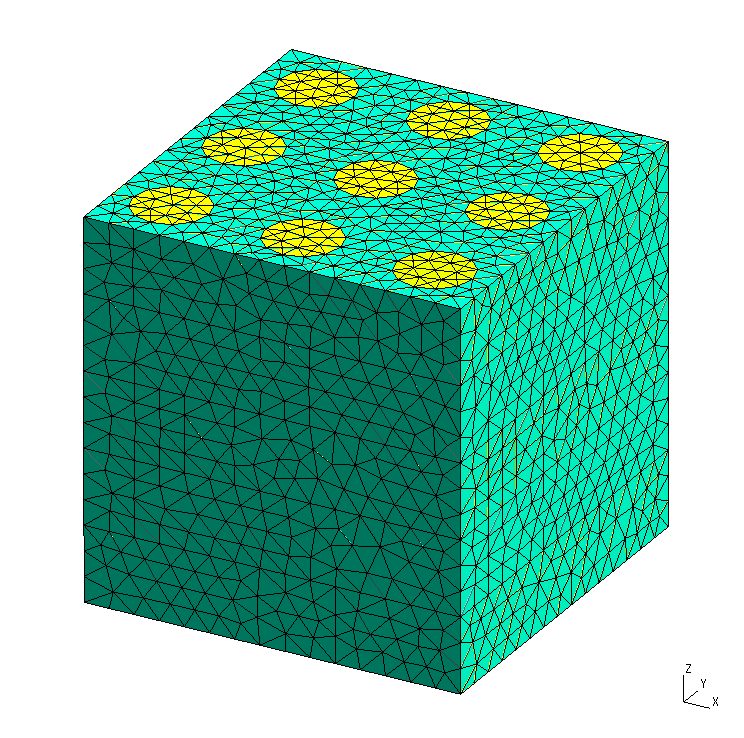
\includegraphics[scale=0.24]{fuel_z5.png}
	\end{minipage}
	\begin{minipage}{0.5\linewidth}
		\centering
		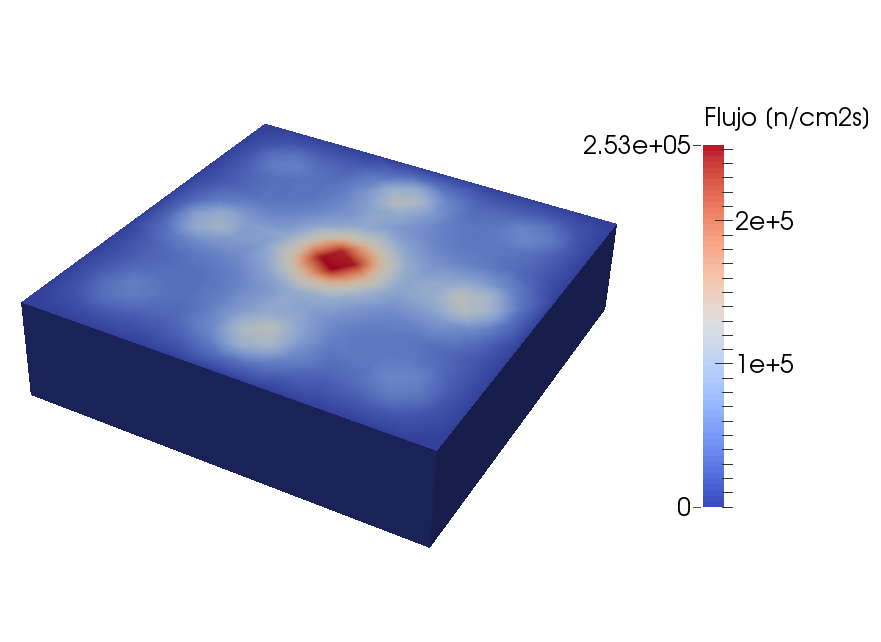
\includegraphics[scale=0.22]{flux_z5.png}
	\end{minipage}
\caption[Núcleo simple en análisis de acoplamiento neutrónico-termohidráulico utilizando \textit{RELAP5} y \textit{Fermi}]
{\textbf{(a)} Esquema de núcleo simple en análisis de acoplamiento neutrónico-termohidráulico utilizando \textbf{RELAP5} y \textbf{Fermi}.
\textbf{(b)} Distribución del flujo neutrónico obtenido en un corte axial a 0.25 $cm$ desde la base del núcleo a principio del ciclo de quemado.
}
\label{fuel_z5}
\end{figure}
El dominio de cálculo termohidráulico consiste en una simplificación de la geometría del núcleo,
considerando un único canal de refrigeración cilíndrico de sección similar a aquella por la que fluye todo el caudal del refrigerante.
Este canal está en contacto con una única estructura que genera energía, 
del mismo diámetro que el que tendrían los pines de los elementos combustibles y altura equivalente a la suma de todos ellos.
Como el modelo es ficticio, el diámetro y la cantidada de pines asumen valores arbitrarios.
La energía total generada en esta estructura es igual a la potencia total generada por el reactor. 
Este tipo de modelos es comúnmente utilizado en análsis de acoplamiento neutrónico-termohidráulico \cite{pumita-relap}.
Si bien la geometría de análisis es artificial, 
es importante contar con modelos de secciones eficaces que representen fielmente la dependencia con las variables de estado termohidráulicas.
Por este motivo se construyeron funciones de $\Sigma$ dependientes en $T_{comb}$, $T_{ref}$, $N_{ref}$ y el valor del quemado $B$
a partir de tablas de secciones eficaces proporcionadas por DIFRA (departamento de DIvisión de Física de Reactores Avanzados de CNEA).

La evolución temporal se discretiza en intervalos de 10 días.
Se definen cinco zonas axiales de acoplamiento.
Con el modelo de resolución previamente comentado, quedan definidas en total veinte incógnitas de acoplamiento.
En la Figura \ref{esquema-fermi-relap} se esquematiza la estrategia para un paso de quemado genérico.
Los mapeos entre las variables termohidráulicas y las secciones eficaces fueron implementados en la función \textit{th2xs} en el código \textit{maestro} \textbf{Newton}.
Las potencias $P_i$ calculadas por el código neutrónico son escaleadas mediante la función $P2p$ a valores $p_i$ en el cálculo de residuos.
Estos valores escaleados se definieron de tal forma que todas las variables de acoplamiento tuvieran magnitudes similares,
para evitar la construcción de matrices mal condicionadas en los métodos de resolución implícitos.
La distribución de potencias que efectivamente \textbf{Newton} envía a al código termohidráulico se define a partir de un nuevo mapeo $p2fp$
en el que se calculan las fracciones de potencia correspondientes a cada zona axial.

\pgfdeclarelayer{bg}    % declare background layer
\pgfsetlayers{bg,main}  % set the order of the layers (main is the standard laye

\begin{figure}[h]
\centering{}
\begin{tikzpicture}[
block1/.style={
	draw,
	fill=white,
	rectangle, 
	minimum width={width("Esclavo 1")+3pt},
	minimum height={17pt},
	font=\small, 
  align=center},
arrow1/.style={
  -{Latex[length=3mm, width=1mm]}
  }
]

% residuos
\node [block1, text width=6em] at (0,6em) (res) {\textbf{Resolución de residuos}};


% programa 1
\node[block1, above of=res, yshift=6em] (e1) {\textbf{Fermi}};

% alpha 1
\node [block1, below left of=e1, yshift=-0.8em, xshift=-9em] (alpha1) {$P_1, P_2, ..., P_5$};

% beta 1
\node [block1, above left of=res, yshift=0.8em, xshift=-9em] (beta1) {$p_1, p_2, ..., p_5$};

% gamma 1
\node [block1, above right of=res, yshift=0.8em, xshift=9em] (gamma1) {$N_{ref,1}, T_{ref,1}, T_{comb,1}, ..., T_{comb,5}$};

% delta 1
\node [block1, below right of=e1, yshift=-0.8em, xshift=9em] (delta1) {$\Sigma_1, \Sigma_2, ..., \Sigma_5$};


% programa 2
\node [block1, below of=res, yshift=-6em] (e2) {\textbf{RELAP5}};

% alpha 2
\node [block1, above left of=e2, yshift=2.8em, xshift=-9em] (alpha2) {$N_{ref,1}, T_{ref,1},$\\$T_{comb,1}, ..., T_{comb,5}$};

% beta 2
%\node [block1, below left of=res, yshift=-0.8em, xshift=-9em] (beta2) {$N_{ref,1}, T_{ref,1}, T_{comb,1}, ..., T_{comb,5}$};

% gamma 2
\node [block1, below right of=res, yshift=-0.8em, xshift=9em] (gamma2) {$p_1, p_2, ..., p_5$};

% delta 2
\node [block1, above right of=e2, yshift=0.8em, xshift=9em] (delta2) {$fp_1, fp_2, ..., fp_5$};

% Conexiones 1
\draw[arrow1] ($(e1.west)$) to[out=180, in=70, distance=2em] (alpha1.north);
\draw[arrow1] ($(alpha1.south)$) to node [midway, anchor=center, left]{\textit{mapeo P2p}} (beta1.north);
\draw[arrow1] ($(beta1.south)$) to[out=-70, in=-180, distance=1.7em] ($(res.west)+(0,0.2em)$);

\draw[arrow1] ($(res.east)+(0,0.2em)$) to[out=0, in=-110, distance=1.7em] ($(gamma1.south)$);
\draw[arrow1] ($(gamma1.north)$) to node [midway, anchor=center, right]{\textit{mapeo th2xs}} (delta1.south);
\draw[arrow1] ($(delta1.north)$) to [out=110, in=0, distance=2em] ($(e1.east)$);

% Conexiones 2
\draw[arrow1] ($(e2.west)$) to[out=180, in=-70, distance=2em] (alpha2.south);
\draw[arrow1] ($(alpha2.north)$) to[out=70, in=-180, distance=3em] ($(res.west)-(0,0.2em)$);
%\draw[arrow1] ($(alpha2.north)$) to node [midway, anchor=center, left]{\textit{mapeo $\alpha_2-\beta_2$}} (beta2.south);
%\draw[arrow1] ($(beta2.north)$) to[out=70, in=-180, distance=1.7em] ($(res.west)-(0,0.2em)$);

\draw[arrow1] ($(res.east)-(0,0.2em)$) to[out=0, in=110, distance=1.7em] ($(gamma2.north)$);
\draw[arrow1] ($(gamma2.south)$) to node [midway, anchor=center, right]{\textit{mapeo p2fp}} (delta2.north);
\draw[arrow1] ($(delta2.south)$) to [out=-110, in=0, distance=2em] ($(e2.east)$);

% Fondo
\begin{pgfonlayer}{bg}    % select the background layer
  % Newton frame
  \draw [blue, rounded corners, thick, dashed, opacity=0.5, fill=blue!10] 
  ($(res.west) + (-16em, 7em)$)
  -- ($(res.west) + (-16em,-7em)$)
  -- ($(res.east) + (16em,-7em)$)
  -- ($(res.east) + (16em,7em)$)
  -- ($(res.west) + (-16em,7em)$);
  % newton
  \node [draw,blue, rounded corners, thick, dashed, opacity=0.5, fill=blue!10] 
  at ($(beta1.west) + (-2em, -2.5em)$) (newton) {\textbf{Newton}};
\end{pgfonlayer}

\end{tikzpicture}
\caption[Instancias de cálculo de las variables relacionadas con cada programa \textit{esclavo}]
{Instancias de cálculo de las variables relacionadas con cada programa \textit{esclavo} en la resolución del problema de acoplamiento neutrónico-termohidráulico.
En este ejemplo los programas \textbf{Fermi} y \textbf{RELAP5} se comunican con \textbf{Newton}.}
\label{esquema-fermi-relap}
\end{figure}

El modelo neutrónico es resuelto con \textbf{Fermi} \cite{fermi}.
\textbf{Fermi} es un código de núcleo que calcula el flujo neutrónico a un grupo de energía a partir de un esquema de elementos finitos de la ecuación \ref{eq-nucleo}.
Las ecuaciones modelos presentadas en \ref{relap-calor}, \ref{relap-masa}, \ref{relap-momento} y \ref{relap-energia},
los modelos de cierre necesarios para formular problemas bien definidos que ajusten a los distintos regímenes de flujo,
y las ecuaciones modelos para las condiciones de borde de cada una de estas ecuaciones,
son resueltas con \textbf{RELAP5}.
\textbf{RELAP5} es un código de análisis de seguridad de reactores nucleares desarrollado por el Laboratorio Nacional de Idaho (INL, por sus siglas en inglés).
\textbf{RELAP5} ha sido validado en cálculos termohidráulicos de reactores nucleares y debido al amplio uso que tiene este código a nivel internacional
se decidió utilizar en la resolución del problema modelado en la presente sección,
para demostrar la posibilidad de uso en acoplamientos mediante la estrategia descripta en el \hyperlink{chapter.2}{Capítulo 2}.
\textbf{RELAP5} resuelve las ecuaciones \ref{relap-calor}, \ref{relap-masa}, \ref{relap-momento} y \ref{relap-energia} a partir de esquemas semi-implícitos de diferencias finitas.

La resolución del sistema acoplado se llevó a cabo utilizando cuatro métodos diferentes.
Cada paso de quemado se consideró convergido cuando la norma infinito del residuo se hizo inferior a una tolerancia $tol$ absoluta prefijada.
Esta tolerancia $tol$ se fijo en $0.1$.
Esta propuesta implica iterar con la solución hasta que el residuo en cada variable caiga por debajo de $0.1$, que es la precisión de los resultados impresos por \textbf{RELAP5}.
Exigir una mayor precisión en la impresión de resultados no es justificable debido a los modelos y las aproximaciones utilizadas.
En todos los métodos se utilizó extrapolación lineal para proponer la semilla $\bar{x}_0^n$ en el cálculo del paso de quemado $n$.
La Figura \ref{figura-relap-fermi} muestra la cantidad de evaluaciones de funciones requerida por cada método para la convergencia de la solución en cada paso de quemado,
y la Tabla \ref{tabla-relap-fermi} integra la cantidad total de evaluaciones y el tiempo consumido por cada uno.

\begin{figure}[h]
  \centering
  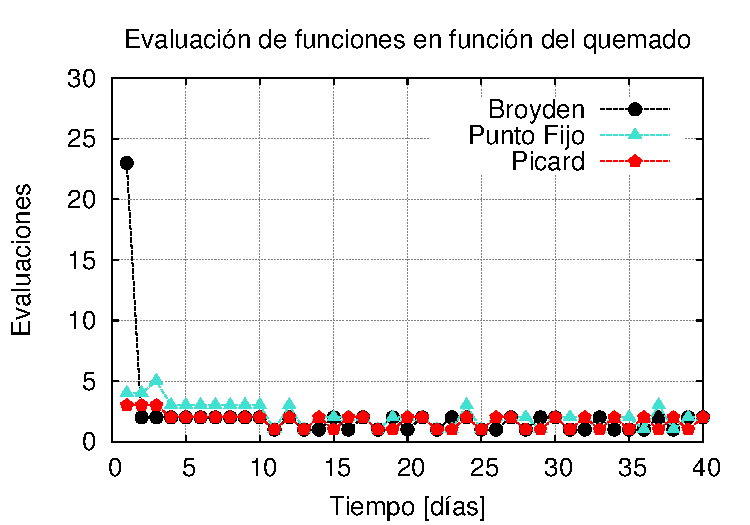
\includegraphics[scale=1]{fermi-relap-feval.pdf}
  \label{figura-relap-fermi}
  \caption[Evaluaciones de funciones en cada paso de quemado en cálculo con \textbf{RELAP5} y \textbf{Fermi}]
  {Evaluaciones de funciones en cada paso de quemado en cálculo con \textbf{RELAP5} y \textbf{Fermi}.}
\end{figure}

\begin{table}[h]
  \centering
  \begin{tabular}{ l r r } \hline
      Método no lineal& Evaluaciones totales & Tiempo total [s]\\ \hline %\hline
      Broyden & 85 & 610 \\ %\hline
      Picard & 68 & 684 \\ %\hline
      Punto fijo & 87 & 628  \\ %\hline
      Secante modificado & 370 & 2663  \\ \hline
   \end{tabular}
   \label{tabla-relap-fermi}
   \caption[Evaluaciones totales y tiempo total requerido por cada método no lineal en cálculo de quemado con \textbf{RELAP5} y \textbf{Fermi}]
   {Evaluaciones totales y tiempo total requerido por cada método no lineal en cálculo de quemado con \textbf{RELAP5} y \textbf{Fermi}.}
\end{table}

El método \textit{Dirichlet-to-Neumann} (iteraciones de \textit{Picard}) es el que consume mayor tiempo de cálculo.
El método del punto fijo demuestra la ventaja de mantener a los diferentes programas \textit{exclavos} corriendo en paralelo y concluye con un tiempo de cálculo inferior.
Se ensayaron diferentes modificaciones del método de la \textit{secante} para el uso en este problema particular.
El esquema implementado requiere la construcción de la matriz jacobiana en el primer paso temporal,
y luego se evalúa si es necesario su reinicialización cada dos pasos temporales,
en base a la cantidad de iteraciones que le toma para converger.
Este método toma excesivas evaluaciones de funciones y recursos de cálculo asociado\footnote{
Si bien el cálculo de la matriz jacobiana es paralelizable,
esta paralelización hubiera requerido la múltiples ejecuciones del mismo programa al mismo tiempo.
Se optó por serializar las sucesivas evaluaciones que requieren su contrucción debido a un criterio de diseño
de mantener controlada la cantidad de ejecuciones de código disparadas por el código \textit{maestro}.
}.
Esquemas con menor frecuencia de reinicio resultan divergentes en algún punto del ciclo de quemado.
Los esquemas con mayor frecuencia de reinicio, como el método de \textit{Newton-Raphson} (que reinicia la matriz jacobiana en cada iteración),
convergen pero requieren muchas más evaluaciones asociadas.
Por último, se utilizó el método de \textit{Broyden} que en previas aplicaciones había demostrado muy buenos resultados.
Si bien este método requiere numerosas evaluaciones en la primera iteración del primer paso de cálculo para la construcción de la matriz jacobiana,
en los siguientes pasos de quemado converge en pocas iteraciones, obteniendo el menor tiempo de cálculo total.
Los métodos \textit{Newton-Krylov} no fueron tenidos en cuenta puesto que hubieran requerido numerosas evaluaciones de funciones
debido a la gran cantidad de incógnitas del sistema.

\subsection*{Acoplamiento neutrónico-termohidráulico utilizando RELAP y PUMA}
\label{3:relap-puma}

La segunda aplicación analizada consiste en el análisis del núcleo del reactor CAREM-25 \cite{carem} durante un ciclo de quemado de 400 días.
CAREM-25 es un reactor integrado de convección natural con generación 100 MW térmicos.
Utiliza agua liviana como refrigerante y uranio enriquecido como combustible, y
cuenta con diseños innovativos en sistemas de seguridad \cite{carem}.
El análisis de este reactor es un problema complejo, con gran cantidad de incógnitas de acoplamiento.

El dominio de cálculo neutrónico consiste en un núcleo de 1.4 metros de altura y 1.312 metros de diámetro equivalente.
Este núcleo está compuesto por 61 elementos combustibles.
Cada elemento combustible posee una sección transversal de forma hexagonal con 127 posiciones, entre las que se disponen barras con material combustible y absorbente.
En la Figura \ref{carem_geom} puede observarse un esquema del núcleo del reactor.
La malla de cálculo utilizada está compuesta por celdas pentahédricas.
Los diferentes colores en la Figura \ref{carem_geom} representan diferentes materiales ficticios homogeneizados por zona en previos cálculos de celda.
Las diferencias corresponden al grado de enriquecimiento de cada combustible y a la posibilidad que algunos tienen de alojar materiales de control.
Las barras de control del Sistema de Ajuste y Control (SAC) se encuentran insertadas hasta la mitad de la longitud activa del núcleo durante todo el ciclo de quemado.
No se detalla la dispoción de materiales porque no se considera relevante para el objetivo de estudio.

\begin{figure}[ht]
	\begin{minipage}{0.5\linewidth}
		\centering
		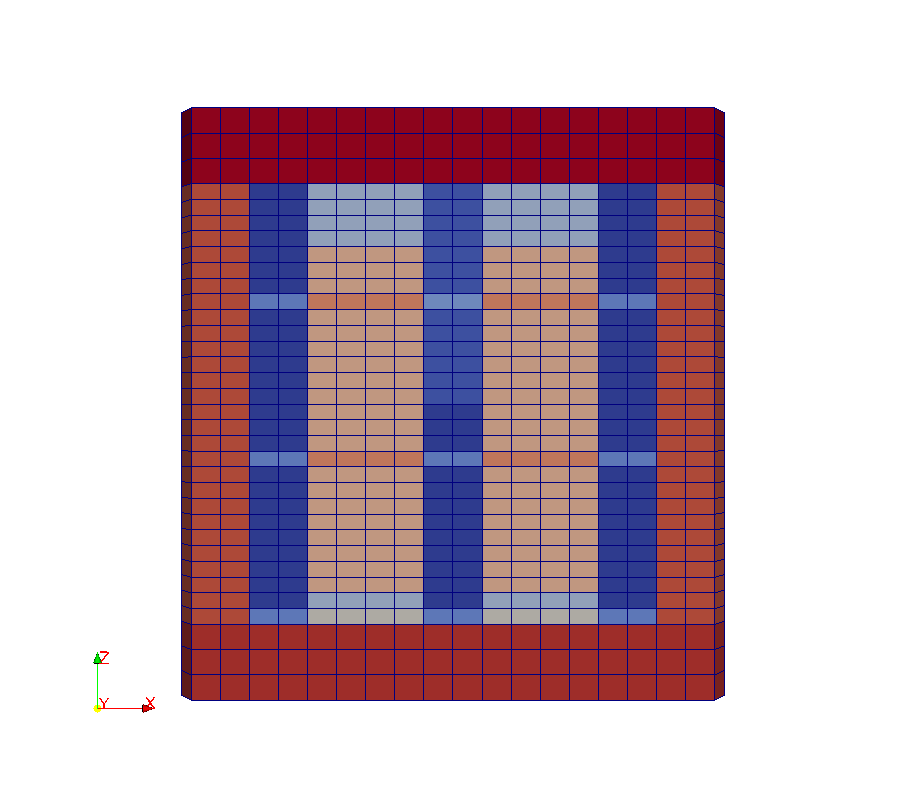
\includegraphics[scale=0.24]{carem_geom_1.png}
	\end{minipage}
	\begin{minipage}{0.5\linewidth}
		\centering
		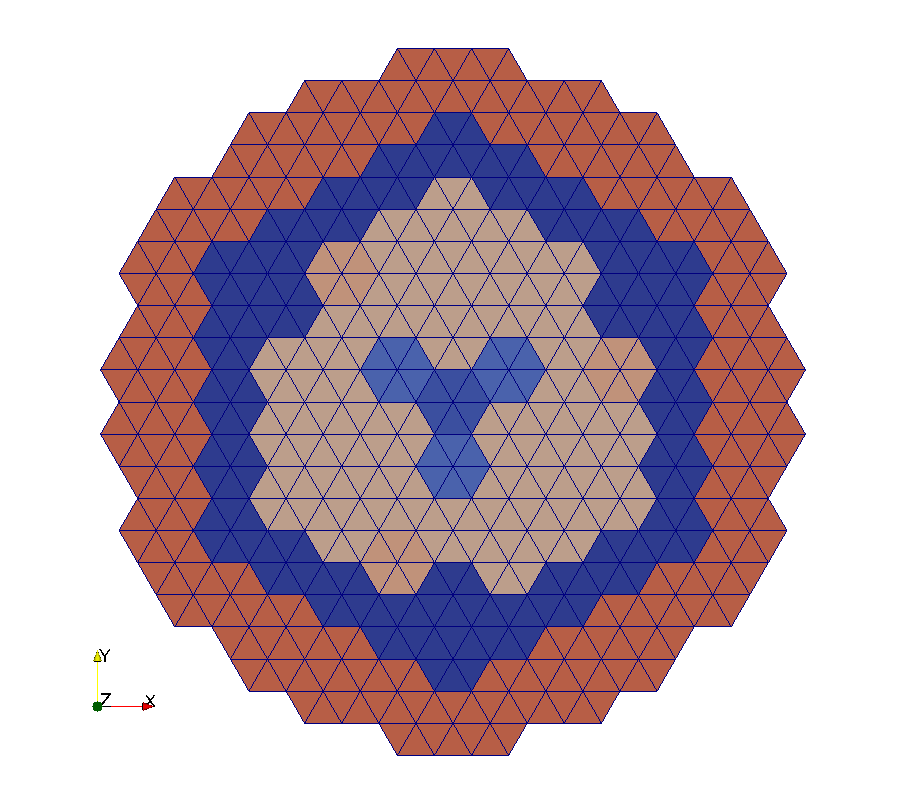
\includegraphics[scale=0.22]{carem_geom_2.png}
	\end{minipage}
\caption[Modelo de núcleo del reactor CAREM-25]
{Modelo de núcleo del reactor CAREM-25:
\textbf{(a)} Corte transversal.
\textbf{(b)} Corte axial.
}
\label{carem_geom}
\end{figure}
La ecuación \ref{eq-nucleo} que modela el flujo neutrónico es resuelta con \textbf{PUMA} \cite{puma} a cinco grupos de energía.
\textbf{PUMA} es un código de núcleo desarrollado por CNEA que calcula el flujo neutrónico a partir de un esquema de diferencias finitas de la ecuación \ref{eq-nucleo}.
El modelo de núcleo desarrollado para su cálculo con \textbf{PUMA} fue proporcionado por DIFRA.

El dominio de cálculo termohidráulico consiste en una simplificación de la geometría del núcleo, similar a la realizada en el ejemplo de análisis previo.
Se modela un único canal de refrigeración en contacto con una estructura de calor que contiene toda la masa de los elementos combustibles.
La longitud de esta estructura es equivalente a la longitud de la suma de todos los pines presentes en los elementos combustibles.
Radialmente, respeta la distribución de material de combustible, \textit{gap} y material de vaina.
Este modelo proviene de una monografía \cite{relap-carem} realizada durante el cursado de \textit{Modelado de sistemas termohidráulicos en reactores mediante códigos de planta}.
Las ecuaciones hidrodinámicas son resueltas con \textbf{RELAP5}.

La evolución temporal se discretiza en intervalos de 5 y 10 días para diferentes simulaciones.
La altura del núcleo se discretiza en tramos de 5 cm, con lo que quedan definidas 28 zonas axiales diferentes que se mantienen acopladas entre ambos modelos.
Como en cada zona axial quedan definidas cuatro incógnitas de acoplamiento, en total existen 112 incógnitas.

Durante la evolución de quemado no se realizó movimiento de barras de control para el mantenimiento de la criticidad.
Se mantuvieron insertadas hasta la mitad del núcleo durante todo el ciclo para que el exceso o la falta de reactividad no sea tan abrupta en los extremos.
El movimiento de barras hubiera incorporado un modelo extra en el acoplamiento\footnote{
Así como la termohidráulica del núcleo genera alteraciones en la distribución de las secciones eficaces en función de la distribución de potencia,
el movimiento de barras generaría también alteraciones en la distribución de las secciones eficaces en función de la distribución de potencia y del $k_{eff}$ del núcleo.
} y aquí no fue considerado por simplicidad.
En la Figura \ref{carem_power} puede observase cómo evoluciona la distribución de potencia en un corte axial a la mitad del núcleo,
y en la Figura \ref{carem_burnup} se observa la evolución de la distribución de quemado correspondiente.
La distribución de potencia se atenúa en el centro y se concentra en los anillos intermedios del núcleo a medida que avanza el ciclo de quemado.

\begin{figure}[ht]
	\begin{minipage}{0.5\linewidth}
		\centering
		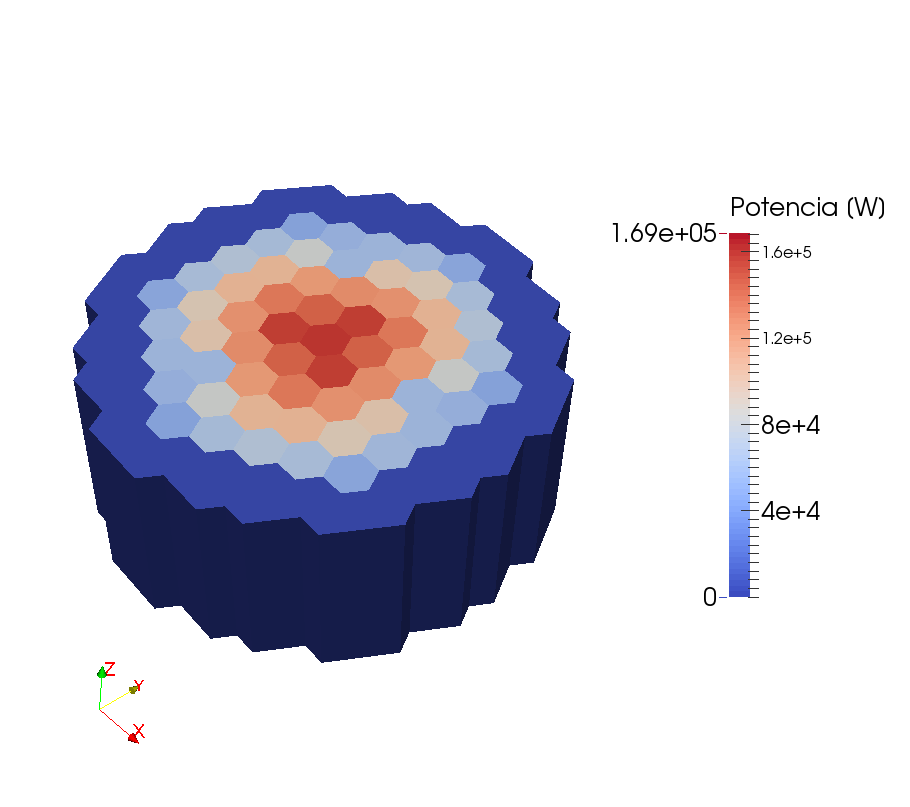
\includegraphics[scale=0.24]{carem_power_10day.png}
	\end{minipage}
	\begin{minipage}{0.5\linewidth}
		\centering
		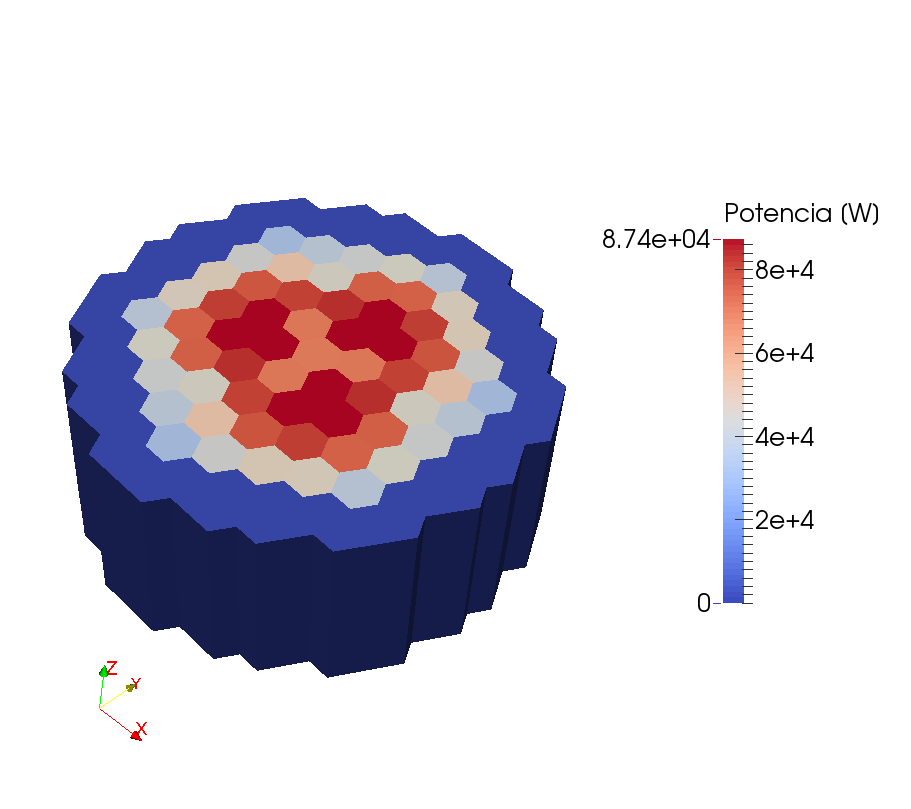
\includegraphics[scale=0.22]{carem_power_400day.png}
	\end{minipage}
\caption[Modelo de núcleo del reactor CAREM-25]
{Evolución de la distribución de potencia en corte axial a la mitad del núcleo:
\textbf{(a)} Distribuión de potencia en día 10.
\textbf{(b)} Distribución de potencia en día 400.
}
\label{carem_power}
\end{figure}

\begin{figure}[ht]
	\begin{minipage}{0.5\linewidth}
		\centering
		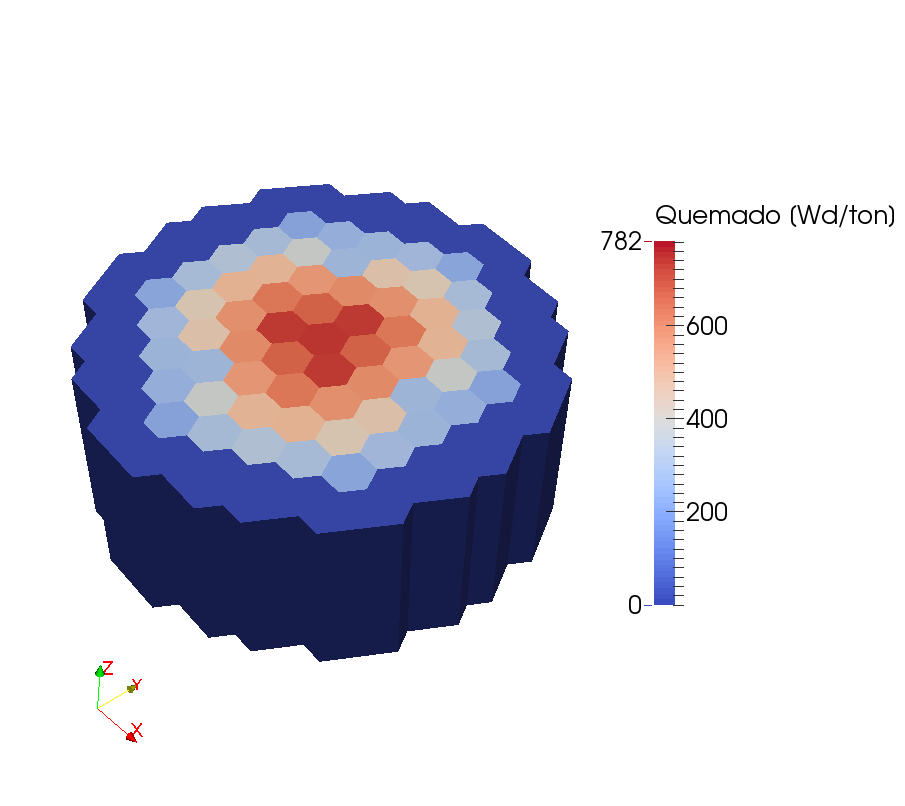
\includegraphics[scale=0.24]{carem_burnup_10day.png}
	\end{minipage}
	\begin{minipage}{0.5\linewidth}
		\centering
		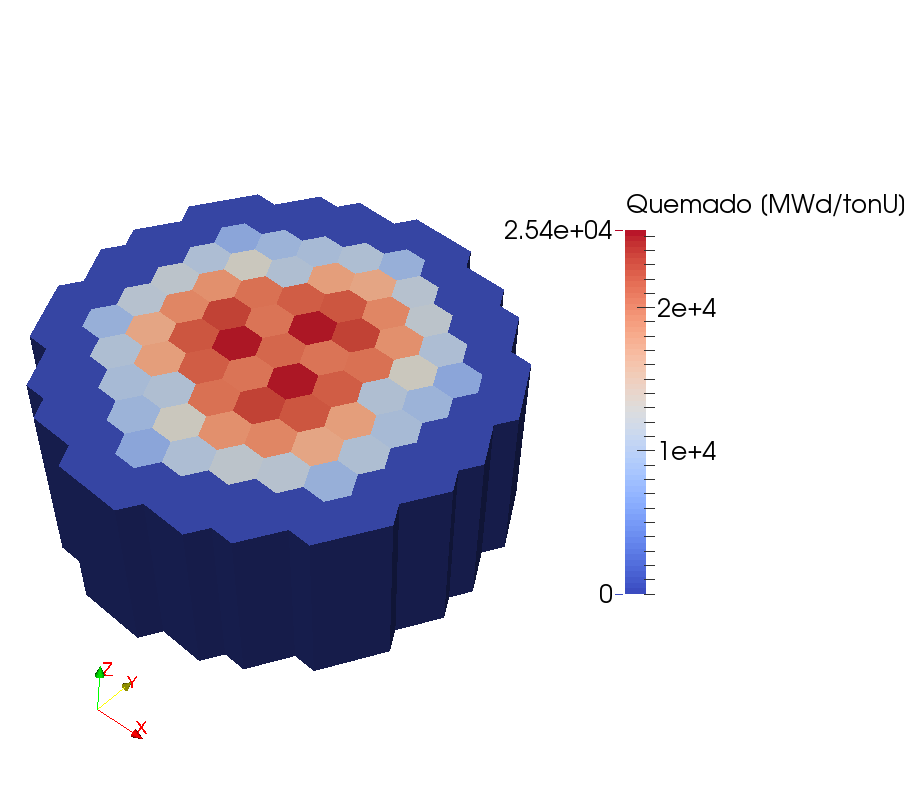
\includegraphics[scale=0.22]{carem_burnup_400day.png}
	\end{minipage}
\caption[Modelo de núcleo del reactor CAREM-25]
{Evolución de la distribución de quemado en corte axial a la mitad del núcleo:
\textbf{(a)} Distribuión de quemado en día 10.
\textbf{(b)} Distribución de quemado en día 400.
}
\label{carem_burnup}
\end{figure}

En la Figura \ref{carem-rho} se observa la evolución de la reactividad a lo largo del ciclo del quemado.
La reactividad está relacionada con el factor de multiplicación $k_{eff}$ de la siguiente forma:
\begin{equation}
\rho = \frac{k_{eff}-1}{k_{eff}}
\end{equation}
y generalmente se expresa en \textit{pcm} (por ciento mil = $10^{-5}$).

\begin{figure}[ht]
	\centering
  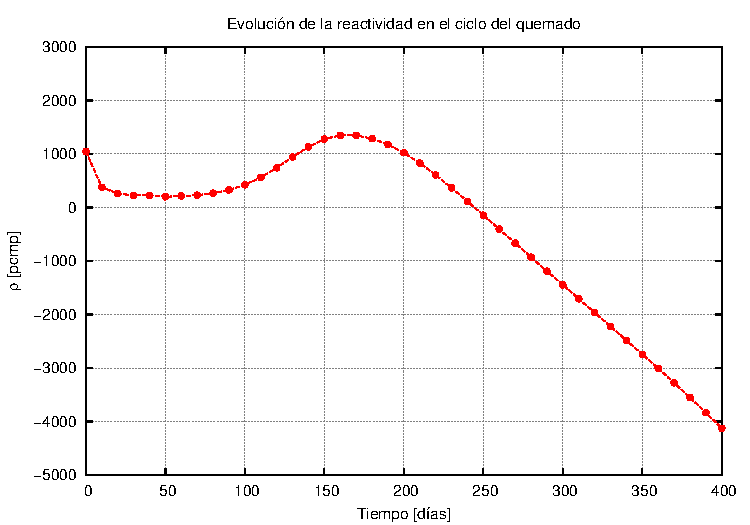
\includegraphics[scale=1]{carem-rho.pdf}
\caption[Evolución de la reactividad en el ciclo de quemado del reactor CAREM-25]
{Evolución de la reactividad en el ciclo de quemado del reactor CAREM-25.
Durante todo el ciclo las barras de control del SAC permanecen insertadas hasta la mitad de la longitud activa del núcleo.}
\label{carem-rho}
\end{figure}

En la resolución del sistema acoplado se consideraron solo tres métodos no lineales debido a las consideraciones comentadas en el ejemplo previo.
También se tomó el mismo criterio de convergencia para cada paso de quemado.

\begin{figure}[h]
  \centering
  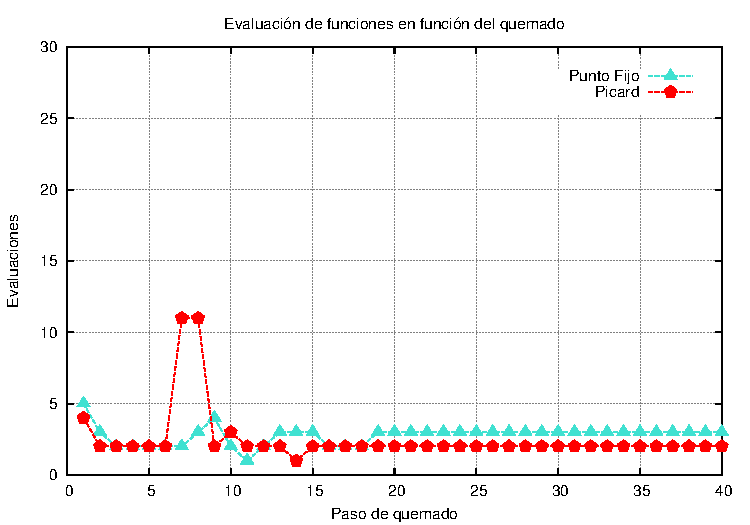
\includegraphics[scale=1]{puma-relap-feval.pdf}
  \label{fig-relap-puma}
  \caption[Evaluaciones de funciones en cada paso de quemado en cálculo con \textbf{RELAP5} y \textbf{Fermi}]
  {Evaluaciones de funciones en cada paso de quemado en cálculo con \textbf{RELAP5} y \textbf{PUMA}.}
\end{figure}

\begin{table}[h]
  \centering
  \begin{tabular}{ l r r } \hline
      Método no lineal & Evaluaciones totales & Tiempo total [s]\\ \hline %\hline
      Picard $\Delta t = 5s$& 243 &  11019 \\ %\hline      
      Picard $\Delta t = 10s$& 104 & 4774 \\ %\hline            
      Punto fijo $\Delta t = 5s$ & 139 & 5415 \\ %\hline            
      Punto fijo $\Delta t = 10s$ & 107 & 3919  \\ \hline      
   \end{tabular}
   \label{tab-relap-puma}
   \caption[Evaluaciones totales y tiempo total requerido por cada método no lineal en cálculo de quemado con \textbf{RELAP5} y \textbf{Fermi}]
   {Evaluaciones totales y tiempo total requerido por cada método no lineal en cálculo de quemado con \textbf{RELAP5} y \textbf{PUMA}.}
\end{table}

comentar doble discretización temporal

Tras múltiples estudios se reporta en la Figura \ref{fig-relap-puma} y en la Tabla \ref{tab-relap-puma} algunos de los resultados obtenidos.
La mayoría de los métodos fueron incapaces de completar el ciclo de quemado asegurando la convergencia fuerte de los resultados en cada paso de evolución.
El método de \textit{Picard} encontró pasos en los que queda estancado, iterando en series de valores que se repiten en ciclos.
Debido a la existencia de estos casos se limitó el método a un máximo de diez iteraciones por paso de quemado,
obligando a continuar con el cálculo en pasos en los que los residuos eran aún un orden de magnitud mayor al fijado por la tolerancia.
Exceptuando esta consideración, ambos métodos explícitos pudieron completar el cálculo a lo largo del ciclo de quemado de manera robusta.
El método del punto fijo aprovecha la ventaja de realizar las evaluaciones de funciones en paralelo y por lo tanto logra completar el cálculo en la menor cantidad de tiempo.

El método implícito de \textit{Broyden} fue estudiado en detalle por haber sido el que mejores resultados había entregado a lo largo de todo el trabajo,
incluyendo el modelo de acoplamiento neutrónico-termohidráulico del apartado previo.
Se hicieron múltiples ensayos incluyendo incialización y reinicialización de matriz jacobiana,
órdenes de extrapolación para el vector de incógnitas $\bar{x}_0^n$ y la matriz $\mathbb{B}_{0}^n$ y
diferentes semillas para arrancar el cálculo.
También se varió el parámetro de discretización temporal.
En las simulaciones con inicialización de la matriz jacobiana, la cual demanda 113 evaluaciones de funciones extra,
las soluciones para cada paso de quemado convergen con un promedio de 1 iteración durante los primeros 20 pasos de quemado aproximadamente.
Este resultado es muy bueno, ya que los métodos explícitos convergen con un promedio de 2.5 iteraciones en cada paso de quemado.
Sin embargo la mayoría de las simulaciones no se pudo completar,
debido a que en algún punto de la evolución aparece una inestabilidad en la convergencia de los resultados en la primera zona acoplada del núcleo.
Esta inestabilidad genera una mala actualización de la matriz de \textit{Broyden} y finalmente el método termina proponiendo valores \textit{guesses} sin sentido físico.
Se desconoce si la inestabilidad encontrada se debe a algún fenómeno físico o a un \textit{bug} del modelo.

En esta sección se ensayaron solo dos modelos de núcleo para estudiar el acoplamiento neutrónico-termohidráulico,
por lo que para obtener conclusiones sobre la ventaja de las técnicas implícitas deberían estudiarse múltiples modelos alternativos.
Cabe destacar que la estrategia de acoplamiento desarrollada provee toda la estructura necesaria para investigar nuevas propuestas.
 % ejemplos de aplicación
\chapter{Conclusiones}
\label{conclusiones}
%~ \chapterquote
%~ {The trouble with the world is that the stupid are cocksure and the intelligent are full of doubt.}
%~ {Bertrand Russell, 1872-1970}
\chapterquote
{El conocimiento no es una vasija que se llena, sino un fuego que se enciende.}
{Plutarco, 46-120}
%~ \chapterquote
%~ {Lo sabio es la meta del alma humana y, a medida que se avanza en sus conocimientos, va alejando a su vez el horizonte de lo desconocido.}
%~ {Heráclito,540-480 a.c.}

En la primera sección de este capítulo se resumen las tareas realizadas en el trabajo de maestría y se presentan los resultados obtenidos más destacados.
En la siguiente sección se comentan las líneas de investigación propuestas para continuar el trabajo.

\section{Logros alcanzados}
\label{logros}

En el trabajo se desarrolló una estrategia genérica que permite resolver problemas fluidodinámicos formulados mediante el Método de Descomposición Disjunta de Dominios.
En la última etapa se extendió la estrategia para cubrir la resolución de problemas acoplados en sistemas complejos que requieren análisis multifísicos.
Esta estrategia de acoplamiento está compuesta por dos etapas:
\begin{enumerate}
\item una primera etapa de modelado, que consiste en la formulación de un problema global, compuesto por subproblemas bien planteados, definición de variables incógnitas y de ecuaciones de residuos (ver \hyperlink{chapter.1}{Capítulo 1});
\item una segunda etapa de resolución, que consiste en la selección de programas de cálculo que resuelvan los subproblemas parciales,
selección del programa \textit{maestro} que resuelva las ecuaciones de residuos, selección de modelos de comunicación, y ejecución de la resolución (ver \hyperlink{chapter.2}{Capítulo 2}).
\end{enumerate}

Durante el trabajo se resolvieron problemas utilizando códigos cuyas fuentes estaban disponibles para realizar implementaciones de funciones de comunicación,
y también utilizando códigos cerrados que se utilizaron como cajas negras de cálculo y se comunicaron mediante manejo de archivos.
En las tareas de acoplamiento se utilizaron dos códigos \textit{maestros}: el código \textbf{Coupling}, en la resolución de problemas formulados mediante el Método de Descomposición Disjunta de Dominios,
y el código \textbf{Newton}, que fue diseñado de forma tal que pudiera utilizarse en la resolución de cualquier tipo de problema que requiriera el acoplamiento de códigos,
y mediante diversos modelos de comunicación.
Las fuentes de \textbf{Newton} fueron publicadas en \textbf{Github} junto con un manual de usuario.

La herramienta de acoplamiento se utilizó en la sección \ref{3:ff} para modelar la dinámica en una fuente fría de neutrones,
acoplando un subdominio de cálculo cero-dimensional y otro bi-dimensional.
El acople permitió analizar el detalle fluídico en el interior de la cavidad conservando la dinámica global de todo el sistema, incluyendo el circuito de enfriamiento.
Se utilizaron diferentes esquemas numéricos de resolución de sistemas no lineales y el método de \textit{Broyden} resultó ser el más eficiente.

El segundo estudio realizado en la sección \ref{3:mockup} fue el análisis del \textit{mockup} del SSP del OPAL,
acoplando un modelo tri-dimensional del arreglo de válvulas presente en la red hidráulica a un modelo cero-dimensional del resto del sistema.
El análisis reveló que la inercia del fluido en la red hidráulica solo influye en el transitorio inicial y
genera un retardo de hasta un segundo en el drenaje del tanque,
respecto de aquellos modelos que no consideran este efecto.
Sin embargo, transcurrido este transitorio, el caudal de descarga se mantiene aproximadamente constante y en todos los modelos es similar a los datos experimentales.
%lo cual verifica el cálculo mediante estudios independientes.
El acoplamiento permitió también estudiar la dinámica del vaciado considerando diferentes válvulas en falla, y los resultados arrojaron diferencias despreciables.
También se pudo confirmar que el gas de relleno de la última porción de las cañerías no genera ningún efecto apreciable durante el vaciado.
En estos análisis se compararon diferentes métodos numéricos de resolución de sistemas no lineales y el método de \textit{Broyden} demostró también ser el más eficiente,
junto con su variante, el método de \textit{Broyden ortonormal}.
Se emplearon diferentes métodos de generación de semillas para el vector de incógnitas $\bar{x}_n$ y la matriz de iteración de \textit{Broyden} $\mathbb{B}_n$ en la iteración $n$,
y se concluyó que el esquema idóneo para resolver este tipo de problemas es utilizar extrapolaciones de alto orden para $\mathbb{B}_n$ en las primeras etapas del cálculo,
y luego solo continuar con extrapolaciones para $\bar{x}_n$.

En la sección \ref{3:redes} se resolvieron sistemas de redes hidráulicas con grandes cantidades de incógnitas.
Los modelos de estudio desarrollados para los diferentes subsistemas fueron sencillos,
de modo de poder estudiar diferentes métodos de resolución de sistemas de ecuaciones utilizando bajo tiempo de cálculo.
En el estudio de sistemas con regímenes de flujo laminar el sistema de ecuaciones a resolver es un sistema lineal.
El método de \textit{Newton-Raphson} y otros métodos \textit{quasi-Newton}, entre los que también se encuentra el método de \textit{Broyden} resultaron ser los más eficientes.
Se propuso la construcción de una semilla para la matriz de cálculo en el método de \textit{Broyden} que acelera la convergencia de los resultados.
En el estudio de sistemas con regímenes de flujo turbulento el sistema de ecuaciones a resolver es un sistema no lineal.
Los métodos de resolución más eficientes resultaron ser nuevamente el método de \textit{Newton-Raphson} y otros métodos \textit{quasi-Newton}
combinados con evaluaciones de \textit{line-searching} entre las iteraciones no lineales.

En la sección \ref{3:extension-nucleo} se extendió la metodología de acoplamiento a la resolución de problemas multifísicos provenientes de modelos de análisis del núcleo de reactores nucleares.
Se desarrolló un modelo de acoplamiento neutrónico-termohidráulico para el estudio de ciclos de quemado de combustibles y se evaluó la eficiencia de resolución de difererentes esquemas numéricos.
%~ Se analizaron dos núcleos diferentes, y en ambos se constató que la técnica de \textit{Picard} comúnmente utilizada no es la más eficiente ya que requiere evaluaciones serializadas
%~ que bien pueden paralelizarse utilizando el método del punto fijo.
Las técnicas explícitas en general resultaron ser robustas, pero en algunos casos se estancaron, iterando en series de valores que se repetían en ciclo,
y en otros requerieron excesivo tiempo de cálculo.
El método de \textit{Broyden} resultó ser eficiente en el primer modelo de núcleo.
En el segundo modelo analizado resultó ser eficiente solo durante la primera mitad del ciclo de quemado,
durante la cual convergía en la mitad de iteraciones de las que requerían los métodos explícitos.
Sin embargo, tras esta primera parte del cálculo encontró inestabilidades.


\section{Trabajos futuros}
\label{trabajos-futuros}

La estrategia de acoplamiento desarrollada permite resolver cualquier tipo de problemas acoplados.
Si bien se ha intentado cubrir diversos tipos de problemas en el área de la fluidodinámica,
incluyendo acoples multi-dimensionales y acoples con baja cantidad de incógnitas y con alta cantidad de incógnitas,
solo se han realizado algunos ensayos en el área multifísica.
Los resultados obtenidos en los modelos de núcleo están lejos de ser concluyentes.
Aquí se abren las puertas a trabajos futuros en los que se investiguen nuevos modelos y esquemas numéricos de resolución.
En primera instancia, sería bueno investigar otros métodos numéricos para la resolución del acoplamiento neutrónico-termohidráulico en los modelos propuestos.
En segunda instancia, podrían ampliarse estos modelos, acoplando al cálculo mayor cantidad de canales de refrigeración.
Sería interesante tambien evaluar el desempeño en el cálculo de la dinámica de núcleos que acoplen el movimiento de las barras de control y el comportamiento de materiales.

Otro trabajo interesante sería evaluar la evolución de la criticidad en el núcleo de reactores que utilizan el vaciado del tanque reflector como SSP.
Este tipo de cálculos implicaría acoplamientos fuertes entre modelos multiescalas del SSP, como el analizado en la sección \ref{3:mockup},
y un acoplamiento débil con el modelo neutrónico, ya que si bien el drenaje del material reflector afecta las secciones eficaces,
la dinámica del núcleo no genera retroalimentación.

También existe otra línea de investigación fuertemente relacionada con el acoplamiento de códigos.
Algunos esquemas de acoplamiento implícito utilizados en el trabajo requirieron la construcción de la matriz jacobiana del sistema de ecuaciones a resolver.
En este trabajo se abordó una metodología de aproximación de sus elementos por diferencias finitas, requiriendo numerosas ejecuciones de código.
Una técnica alternativa que no ha sido investigada es la de diferenciación automática \cite{griewank-ad}.
La diferenciación automática requiere implementaciones en el código fuente del programa de cálculo utilizado,
el cual en lugar de devolver al código \textit{maestro} que lo está llamando sólo el valor de las variables incógnitas,
también debe devolver el valor de sus derivadas con respecto a las variables independientes requeridas
(que en este caso, deberían ser las variables que el código \textit{maestro} le envía como dato).
Esta técnica permitiría construir la matriz jacobiana de manera mucho más rápida y precisa,
con la consecuente aceleración en la convergencia de los resultados.
 % conclusiones

\appendix
\chapter{Descripción del código maestro \textbf{Coupling}}
\label{C:coupling}
%\chapterquote{Negociemos Don Inodoro}{Fernando de la R\'{u}a, 2001}

\textbf{Coupling} es un código escrito en \textit{Fortran 90}, desarrollado por Jorge Leiva, Pablo Blanco y Gustavo Buscaglia.
Fue diseñado como programa \textit{maestro} en las funciones de acoplamiento explícito e implícito,
estableciendo la comunicación con diversos programas \textit{esclavos} mediante funciones de MPI.
Su desempeño fue validado en diversos trabajos de acoplamiento \cite{coup-0d3d} \cite{coup-black} \cite{coup-hyd} \cite{coup-strong}.

\section{Modelado de problemas acoplados}
\label{ap1:definicion}
El programa \textbf{Coupling} resuelve problemas que fueron formulados mediante el Método de Descomposición Disjunta de Dominios descripto en el \hyperlink{chapter.1}{Capítulo 1}.
El esquema de resolución fue diseñado de tal forma que se permite que las interfaces de acoplamiento cuenten con múltiples pares de incógnitas vectoriales en diferentes nodos.
Las principales variables en la definición de un problema son las siguientes:
\begin{itemize}
\item Cantidad de subdominios acoplados (variable \textit{Ncomp}).
\item Cantidad de uniones globales (variable \textit{Nbond}).
\item Cantidad de superficies en cada subdominio (variable \textit{Nsupc}).
\item Matriz de conectividades entre las interfaces de diferentes subdominios (variable con numeraciones locales \textit{Localsur} y globales \textit{Incid}.
\item Cantidad de pares de variables incógntias en cada interfaz (variable \textit{Npair}).
Se supone que cada incógnita de cada interfaz está acompañada de otra variable incógnita relacionada con su gradiente.
Por ejemplo, \textit{temperatura} y \textit{flujo de calor}, o \textit{velocidad} y \textit{presión}.
\item Cantidad de nodos con incógnitas en cada interfaz (variable \textit{Nodpair}).
\item Cantidad de componentes escalares en cada nodo (variable \textit{Npairc}).
\item Tipo de condición de borde para cada nodo (variable \textit{indexbc}).
Las opciones posibles son condiciones de borde \textit{esenciales} (tipo \textit{Dirichlet}) o \textit{naturales} (tipo \textit{Neumann}), y deben establecerse por separado para cada subdominio.
\end{itemize}
Para que el problema de acoplamiento quede bien definido,
todos estos datos deben ser provistos en el archivo de configuración \texttt{mesh.cfg} utilizando palabras claves específicas.
Además, debe proveerse un archivo de configuración extra, el arhivo \texttt{couple.cfg}.
En este archivo se detalla el método de acoplamiento a utilizar en la resolución del problema,
y sus diferentes parámetros específicos.
También se detallan los parámetros necesarios en problemas de evolución.

En la sección \ref{ap1:ejemplo} se describe como ejemplo la formulación utilizada en una de las aplicaciones analizadas en el \hyperlink{chapter.3}{Capítulo 3}.

\section{Metodología de resolución}
\label{ap1:resolucion}

El archivo \texttt{src/couple\_ddm.for} contiene la estructura principal del programa.
El modelo de comunicación entre programas implementado es el de paso de mensajes entre programas ejecutados en modos SISD o SIMD.
Conforme a la estrategia de acoplamiento descripta en el \hyperlink{chapter.2}{Capítulo 2}, se siguen los siguientes pasos:
\begin{enumerate}
\item Lectura de archivos de datos \texttt{mesh.cfg} y \texttt{couple.cfg}.
\item Inicialización de las funciones de MPI y publicación de puertos de conexión.
\item Establecimiento de la comunicación con los diferentes programas esclavos.
\item Envío de datos generales del problema a los programas \textit{esclavos} para chequeo de compatibilidad de datos.
\item Ingreso en el bucle de evolución.
\begin{enumerate}
\item Envío de valores \textit{guess} para las condiciones de borde de cada subdominio a cada programa \textit{esclavo}.
\item Recepción de valores calculados para las incógnitas de cada subdominio de cada programa \textit{esclavo}.
\item Resolución de las ecuaciones de residuos \ref{ecuaciones-residuos}.
\item Evaluación de la convergencia:
\begin{itemize}
\item si los resultados están convergidos el problema puede continuar con el siguiente paso de evolución;
\item si los resultados no están convergidos, es necesario proponer nuevos valores \textit{guess} y reiniciar el cálculo.
\end{itemize}
\item Envío de orden de avance o de reinicio a cada programa \textit{esclavo}.
\end{enumerate}
\item Finalización del bucle de evolución.
\item Cierre de las conexiones con los programas \textit{esclavos} y finalización.
\end{enumerate}
Los pasos descriptos requieren una arquitectura de acoplamiento específica montada en los códigos \textit{esclavos}, la cual fue comentada en la sección \ref{2:arquitectura-mpi}.

\section{Ejemplo de uso}
\label{ap1:ejemplo}

A continuación se comenta la formulación del problema analizado en la sección \ref{3:mockup}:
\textit{Análisis del segundo sistema de parada de un reactor de investigación}.
Se definen dos subdominios: el primero es el subsistema tri-dimensional arreglo de válvulas y el segundo es el subsistema cero-dimensional del tanque del reactor y porción superior de la red hidráulica.
Existe una única unión entre ambos subdominios, la \textit{Unión 1}.
Es necesario definir una numeración global de interfaces de acoplamiento.
El subsistema tri-dimensional contiene la interfaz global \textit{Interfaz 1} y el subsistema cero-dimensional contiene la interfaz global \textit{Interfaz 2}.
En cada interfaz existe un solo par de variables acopladas, el par \textit{caudal-presión}.
El \textit{caudal} es impuesto como condición de borde \textit{esencial} al \textit{Subdominio 1} y la \textit{presión} como condición de borde \textit{natural} al \textit{Subdominio 2}.
La Figura \ref{ra10-coupling} resume las definiciones previas.

\begin{figure}[h]
\centering{}
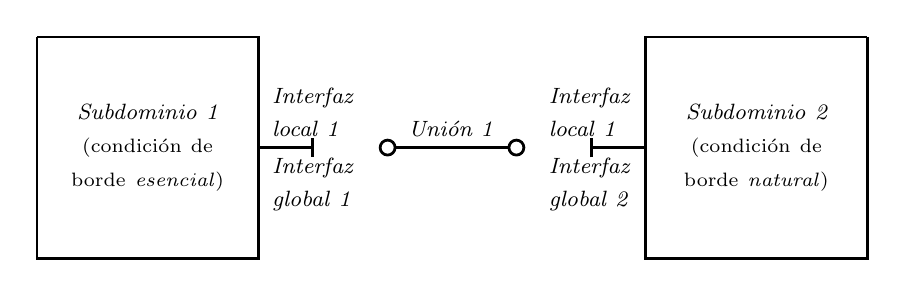
\begin{tikzpicture}

% Dummy
%\node at (0,6em) (dummy) {}; % blank space

% Unión
\node at (-3em,0em) (u0) {};
\node at ( 3em,0em) (u1) {};
\draw[line width=1pt, o-o] (u0) -- (u1) node [midway, sloped, anchor=center, above]{\footnotesize \textit{Unión 1}};

% Box 1
\node at (-15em,4em) (b0) {};
\node at (-15em,-4em) (b1) {};
\node at (-7em,-4em) (b2) {};
\node at (-7em,4em) (b3) {};
\draw[line width=1pt, -] (b0.center) -- (b1.center) -- (b2.center) -- (b3.center) -- (b0.center);
\node [text width=7em, align=center] at (-11em,0) (s1) {\footnotesize \textit{Subdominio 1} \scriptsize(condición de borde \textit{esencial})};

% Box 2
\node at (15em,4em) (b0) {};
\node at (15em,-4em) (b1) {};
\node at (7em,-4em) (b2) {};
\node at (7em,4em) (b3) {};
\draw[line width=1pt, -] (b0.center) -- (b1.center) -- (b2.center) -- (b3.center) -- (b0.center);
\node [text width=7em, align=center] at (11em,0) (s2) {\footnotesize \textit{Subdominio 2} \scriptsize(condición de borde \textit{natural})};

% Interfaz global 1
\node at (-7em,0em) (i10) {};
\node at (-5em,0em) (i11) {};
\draw[line width=1pt, -|] (i10.center) -- (i11.center) node [pos=1.0, text width=3em, above]{\footnotesize \textit{Interfaz local 1}}
node [pos=1.0, text width=3em, below]{\footnotesize \textit{Interfaz global 1}};

% Interfaz global 2
\node at (7em,0em) (i10) {};
\node at (5em,0em) (i11) {};
\draw[line width=1pt, -|] (i10.center) -- (i11.center) node [pos=1.0, text width=3em, above]{\footnotesize \textit{Interfaz local 1}}
node [pos=1.0, text width=3em, below]{\footnotesize \textit{Interfaz global 2}};

\end{tikzpicture}
\caption[Definición del problema de acoplamiento en el SSP de un reactor de investigación]
{Definición del problema de acoplamiento en el Segundo Sistema de Parada del reactor de investigación investigado en la sección \ref{3:mockup}.}
\label{ra10-coupling}
\end{figure}

Las siguientes líneas conforman el archivo de configuración \texttt{mesh.cfg}:

\begin{Verbatim}[frame=single,commandchars=\\\{\}]
\textcolor{Gray}{! Nombre del problema}
\textcolor{Red}{*TITLE}
\textcolor{OliveGreen}{manifold mockup OPAL}

\textcolor{Gray}{! Número de subdominios}
\textcolor{Red}{*NUMBER_OF_COMPONENTS}
\textcolor{OliveGreen}{2     }\textcolor{Gray}{! Subdominio 3D y subdominio 0D}

\textcolor{Gray}{! Cantidad de interfaces en cada subdominio}
\textcolor{Red}{*NUMBER_OF_COMPONENT_INTERFACES}
\textcolor{OliveGreen}{1     }\textcolor{Gray}{! Subdominio (1): 1 interfaz}
\textcolor{OliveGreen}{1     }\textcolor{Gray}{! Subdominio (2): 1 interfaz}

\textcolor{Gray}{! Uniones en cada componente}
\textcolor{Red}{*CONECTIVITY_BETWEEN_COMPONENT_INTERFACES}
\textcolor{OliveGreen}{1 1   }\textcolor{Gray}{! Subdominio (1); Interfaz local (1): Unión 1}
\textcolor{OliveGreen}{2 1   }\textcolor{Gray}{! Subdominio (2); Interfaz local (1): Unión 1}

\textcolor{Gray}{! Pares de variables en cada componente}
\textcolor{Red}{*PAIR_VARIABLES_NUMBER_BY_COMPONENT_INTERFACE}
\textcolor{OliveGreen}{1     }\textcolor{Gray}{! Subdominio (1); interfaz local (1): 1 par}
\textcolor{OliveGreen}{1     }\textcolor{Gray}{! Subdominio (2); interfaz local (1): 1 par}

\textcolor{Gray}{! Componentes escalares en cada par de variables}
\textcolor{Red}{*PAIR_VARIABLES_NUMBER_OF_COMPONENTS}
\textcolor{OliveGreen}{1     }\textcolor{Gray}{! Subdominio (1); interfaz (1); par (1): 1 componente escalar}
\textcolor{OliveGreen}{1     }\textcolor{Gray}{! Subdominio (2); interfaz (1); par (1): 1 componente escalar}

\textcolor{Gray}{! Tipo de condición de borde en cada par}
\textcolor{Red}{*BOUNDARY_CONDITION_TYPE_BY_COMPONENT_PAIRS}
\textcolor{OliveGreen}{1     }\textcolor{Gray}{! Subdominio (1); interfaz (1); par (1): tipo Dirichlet (1)}
\textcolor{OliveGreen}{-1    }\textcolor{Gray}{! Subdominio (2); interfaz (1); par (1): tipo Neumann (-1)}

\textcolor{Gray}{! Cantidad de nodos en cada par de variables}
\textcolor{Red}{*PAIR_VARIABLES_NUMBER_OF_NODES}
\textcolor{OliveGreen}{1     }\textcolor{Gray}{! Subdominio (1); interfaz (1); par (1): 1 nodo}
\textcolor{OliveGreen}{1     }\textcolor{Gray}{! Subdominio (2); interfaz (1); par (1): 1 nodo}

\textcolor{Gray}{! Finalización}
\textcolor{Red}{*END}
\end{Verbatim}

Las siguientes líneas en el archivo de configuración \texttt{couple.cfg} definen la metodología numérica de resolución:

\begin{Verbatim}[frame=single,commandchars=\\\{\}]
\textcolor{Gray}{! Parámetro de evolución inicial}
\textcolor{Red}{*INITIAL_CONTINUATION_PARAMETER}
\textcolor{OliveGreen}{0.0}

\textcolor{Gray}{! Parámetro de evolución final}
\textcolor{Red}{*FINAL_CONTINUATION_PARAMETER}
\textcolor{OliveGreen}{15.0}

\textcolor{Gray}{! Cantidad de pasos de evolución}
\textcolor{Red}{*NUMBER_OF_CONTINUATION_STEPS}
\textcolor{OliveGreen}{1500}

\textcolor{Gray}{! Maxima cantidad de iteraciones del método de acoplamiento en cada}
\textcolor{Gray}{paso}
\textcolor{Red}{*MAXIMUM_NONLINEAR_ITERATIONS}
\textcolor{OliveGreen}{800}

\textcolor{Gray}{! Método de acoplamiento}
\textcolor{Red}{*NONLINEAR_SOLVER}
\textcolor{OliveGreen}{2} \textcolor{Gray}{! Broyden}

\textcolor{Gray}{! Tolerancia absoluta en residuos de variables acopladas}
\textcolor{Red}{*ABSOLUTE_TOLERANCE}
\textcolor{OliveGreen}{1.0e-15}

\textcolor{Gray}{! Tolerancia relativa en residuos de variables acopladas}
\textcolor{Red}{*TOLERANCE_NONLINEAR}
\textcolor{OliveGreen}{1.0e-08}

\textcolor{Gray}{! Iteraciones lineales máximas en la resolución de sistemas}
\textcolor{Gray}{algebraicos definidos en métodos implícitos}
\textcolor{Red}{*MAXIMUM_LINEAR_ITERATIONS}
\textcolor{OliveGreen}{800}

\textcolor{Gray}{! Pasos entre las reinicializaciones de la matriz jacobiana}
\textcolor{Red}{*JACOBIAN_INITIALIZATION}
\textcolor{OliveGreen}{100}

\textcolor{Gray}{! Parámetro de perturbación en cálculo de la matriz jacobiana mediante}
\textcolor{Gray}{diferencias finitas}
\textcolor{Red}{*JACOBIAN_PERTURBATION_PARAMETER}
\textcolor{OliveGreen}{0.1}

\textcolor{Gray}{! Máxima cantidad de evaluaciones de funciones en cada paso}
\textcolor{Red}{*MAXIMUM_FUNCTION_EVALUATIONS}
\textcolor{OliveGreen}{10000}

\textcolor{Gray}{! Órden de extrapolación de variables incógnitas}
\textcolor{Red}{*STATE_VARS_EXTRAPOLATION_ORDER}
\textcolor{OliveGreen}{1}

\textcolor{Gray}{! Órden de extrapolación de matriz jacobiana}
\textcolor{Red}{*JACOBIAN_EXTRAPOLATION_ORDER}
\textcolor{OliveGreen}{0}

\textcolor{Gray}{! Finalización}
\textcolor{Red}{*END}
\end{Verbatim}

\chapter{Descripción del código maestro \textbf{Newton}}
\label{C:newton}
%\chapterquote{Negociemos Don Inodoro}{Fernando de la R\'{u}a, 2001}

\textbf{Newton} es un código escrito en \texttt{C++} desarrollado durante la maestría,
publicado en \textbf{Github} \cite{github} bajo Licencia Pública General (GPL por sus siglas en inglés, \textit{Public General License}) del Proyecto GNU colaborativo de software libre.
Fue diseñado como programa \textit{maestro} con un propósito general, de forma que permita resolver cualquier tipo de ecuaciones acopladas,
parcialmente resueltas por códigos \textit{esclavos}.
Algunos ejemplos de los problemas que pueden resolverse con \textbf{Newton} son los siguientes:
\begin{itemize}
\item Cálculos formulados con el Método de Doscomposición Disjunta de Dominios: 
acoplamientos fluidodinámicos multiescala, con o sin transferencia de calor, como los presentados en las secciones \ref{3:ff}, \ref{3:mockup} y \ref{3:redes}.
\item Cálculos multifísicos: acoplamiento fluido-estructura, acoplamiento neutrónico-termohidráulico, como los presentados en la sección \ref{3:extension-nucleo}.
También podrían pensarse modelos de núcleo completo (\textit{full core models}), acoplando el comportamiento de los materiales a la dinámica neutrónica-termohidráulica y otros fenómenos de interés.
\end{itemize}

\section{Principales características}
\label{ap2:main-features}

\subsection*{Archivo de configuración}
\label{ap2:parser}

La ejecución de \textbf{Newton} requiere el archivo de configuración \texttt{newton.config} en el que debe detallarse la formulación del problema a resolver,
la forma de comunicación con cada código \textit{esclavo}, los mapeos utilizados, y métodos numéricos y demás parámetros asociados a la resolución del sistema \ref{sistema-simple}.
El formato de entrada fue pensado de forma tal que resulte simple e intuitivo al usuario.
Las funciones implementadas en la clase \texttt{Parser} se encargan de analizar las diferentes palabras claves ingresadas y sus atributos.
Se desarrolló un manual de comandos de entrada \cite{newton-user-manual}.

\subsection*{Mapeos}
\label{ap2:mappers}

En ciertas formulaciones las variables de acoplamiento pueden ser expresadas bajo transformaciones en las diferentes ecuaciones acopladas.
Por ejemplo, en acoplamientos fluidodinámicos es común que en algunos modelos se calculen velocidades medias en interfaces de acople
y que en otros modelos se calculen valores de caudales.
En estos casos es necesario realizar mapeos \textit{velocidad-caudal}.
En otros tipos de problemas también es necesario realizar mapeos.
En acoplamiento neutrónico-termohidráulico, por ejemplo, las variables de cálculo del programa termohidráulico podrían ser densidades y termperaturas,
pero el programa neutrónico utiliza como variables secciones eficaces, que dependen de ellas.
Además, las variables transformadas podrían ser condensadas o multiplicadas.
Aquí podría pensarse un mapeo \textit{termohidráulico-secciones eficaces}.

En general, los mapeos son transformaciones simples de las variables de acoplamiento, y pueden extraerse de la resolución de las ecuaciones parciales,
definiendo ecuaciones extras que pueden ser resueltas por el programa \textit{maestro}.
Debido a esta generalización, es necesario definir cuál va a ser la variable acoplada utilizada para resolver el sistema de residuos \ref{sistema-simple}.
Diferentes mapeos pueden ser utilizados para diferentes códigos \textit{esclavos}, ya sea para adecuar variables \textit{guess} o variables calculadas.
Su implementación requiere una mínima programación en funciones listas para ser utilizadas pertenecientes a la clase \texttt{Mapper}.
Luego deben ser incluidos mediante palabras claves en el archivo de configuración \texttt{newton.config}.

\subsection*{Modelos de comunicación}
\label{ap2:comm}

Con la finalidad de poder establecer conexiones con programas \textit{esclavos} cuyos códigos fuente no están disponibles,
se incorporaron diferentes modos de comunicación, conforme a la estrategia descripta en el \hyperlink{chapter.2}{Capítulo 2}:
\begin{itemize}
\item Comunicación por MPI entre programas ejecutados en simultáneo o entre programas ejecutados de manera independiente, cuando es posible acceder al código fuente.
\item Comunicación por lectura y escritura de archivos con programas sin acceso al código fuente.
\end{itemize}
Todas estas funciones fueron implementadas en la clase \texttt{Communicator}.
\textbf{Newton} puede ser ejecutado en múltiples procesos de modo que la conexión mediante manejo de archivos sea paralelizada.
Las tareas se distribuyen automáticamente de forma eficiente conforme a la cantidad de procesos lanzados por el usuario.

\subsection*{Métodos numéricos}
\label{ap2:num-met}

\textbf{Newton} puede resolver acoplamientos utilizando diferentes métodos numéricos:
\begin{itemize}
\item Métodos explícitos:
\begin{itemize}
\item método \textit{Picard} simple;
\item método \textit{Picard} combinado.
\end{itemize}
\item Métodos implícitos:
\begin{itemize}
\item método de \textit{Newton-Raphson};
\item método de \textit{Shamanskii};
\item método de \textit{Broyden}.
\end{itemize}
\end{itemize}
A futuro sería posible implementar otros métodos en la clase \texttt{Solver}.
Los sistemas algebraicos resultantes en los métodos implícitos son resueltos mediante la biblioteca \textbf{PETSc} \cite{petsc-web-page} altamente eficiente para este tipo de cálculos.

\subsection*{Manejo de errores}
\label{ap2:error}

El manejo eficiente de errores fue pensado como una de las características principales durante el diseño del programa,
debido a la complejidad de conexiones y consecuente diversidad en origen de fallas.
Cualquier error generado comienza la siguiente cascada de eventos:
\begin{enumerate}
\item Devolución de un mensaje correspondiente en la salida estándar.
\item Comunicación del error a todos los procesos de \textbf{Newton}.
\item Envío de órden de aborto a los programas \textit{esclavos} por parte del proceso \textit{raiz}.
\item Finalización de las tareas.
\end{enumerate}

\subsection*{Depuración}
\label{ap2:debug}

Se desarrolló un visualizador genérico en la clase \texttt{Debugger} para realizar seguimiento de la evolución de las variables pertenecientes a las diferentes clases implementadas.
El usuario puede requerir su uso en clases específicas mediante palabras claves ingresadas en el archivo de configuración para la ejecución de \textbf{Newton}.
\texttt{Debugger} va imprimiendo la salida requerida en archivos particulares para cada clase.

\subsection*{Validación}
\label{ap2:bench}

Las funciones implementadas y la metodología de cálculo fueron puestas a prueba exitosamente en la resolución de sistemas de ecuaciones lineales y no lineales acopladas.
Las mismos pueden encontrarse dentro de la carpeta \texttt{examples} en el directorio principal de \textbf{Newton}.
Se verificó el correcto funcionamiento de los diferentes tipos de comunicación, de las intancias de mapeos y de los distintos métodos numéricos implementados para la resolución del sistema de ecuaciones de residuos.

\section{Modelado de problemas acoplados}
\label{ap1:definicion}

\textbf{Newton} resuelve problemas que comprenden algún sistema de ecuaciones acopladas, en el que las ecuaciones son resueltas por separado por diferentes programas.
Conforme a la estrategia de acoplamiento extendida comentada en la sección \ref{3:strategy-extended}, 
es necesario definir qué variables van a ser datos y qué variables van a ser incógnitas para cada subsistema de análisis.
Como existe la posibilidad de transformaciones previas o posteriores a la resolución del sistema de ecuaciones de residuos característico de cada problema,
es necesario además definir en forma clara cuáles van a ser las variables transformadas y los mapeos.
Para organizar esta formulación en forma clara \texttt{Newton} trabaja con cuatro instancias de variables para cada programa \textit{esclavo}:
las instancias $\alpha$, $\beta$, $\gamma$ y $\delta$.

\subsection*{Alfas, betas, gammas y deltas}
\label{ap1:abgd}

Existen cuatro instancias de variables para cada programa \textit{esclavo}:
\begin{enumerate}
\item Instancia $\alpha$: corresponde al valor crudo de las variables calculadas por el programa.
\item Instancia $\beta$: corresponde al valor transformado de las variables $\alpha$.
En el caso de que no se haya definido una transformación, se utiliza la transformación de identidad por defecto.
Las variables $\beta$ están listas para ser utilizadas en el cálculo de residuos.
\item Instancia $\gamma$: corresponde a los valores \textit{guess} generados por \textbf{Newton} para ese programa.
\item Instancia $\delta$: corresponde a los valores $\gamma$ transformados, utilizando también la transformación de identidad por defecto.
\end{enumerate}
La Figura \ref{fig:abgd} esquematiza lo expresado.

\pgfdeclarelayer{bg}    % declare background layer
\pgfsetlayers{bg,main}  % set the order of the layers (main is the standard laye

\begin{figure}[h]
\centering{}
\begin{tikzpicture}[
block1/.style={
	draw,
	fill=white,
	rectangle, 
	minimum width={width("Esclavo 1")+3pt},
	minimum height={17pt},
	font=\small, 
  align=center},
arrow1/.style={
  -{Latex[length=3mm, width=1mm]}
  }
]

% residuos
\node [block1, text width=6em] at (0,6em) (res) {\textbf{Resolución de residuos}};


% programa 1
\node[block1, above of=res, yshift=6em] (e1) {\textbf{Esclavo 1}};

% alpha 1
\node [block1, below left of=e1, yshift=-0.8em, xshift=-9em] (alpha1) {\textbf{variables} $\alpha_1$};

% beta 1
\node [block1, above left of=res, yshift=0.8em, xshift=-9em] (beta1) {\textbf{variables} $\beta_1$};

% gamma 1
\node [block1, above right of=res, yshift=0.8em, xshift=9em] (gamma1) {\textbf{variables} $\gamma_1$};

% delta 1
\node [block1, below right of=e1, yshift=-0.8em, xshift=9em] (delta1) {\textbf{variables} $\delta_1$};


% programa 2
\node [block1, below of=res, yshift=-6em] (e2) {\textbf{Esclavo 2}};

% alpha 2
\node [block1, above left of=e2, yshift=0.8em, xshift=-9em] (alpha2) {\textbf{variables} $\alpha_2$};

% beta 2
\node [block1, below left of=res, yshift=-0.8em, xshift=-9em] (beta2) {\textbf{variables} $\beta_2$};

% gamma 2
\node [block1, below right of=res, yshift=-0.8em, xshift=9em] (gamma2) {\textbf{variables} $\gamma_2$};

% delta 2
\node [block1, above right of=e2, yshift=0.8em, xshift=9em] (delta2) {\textbf{variables} $\delta_2$};

% Conexiones 1
\draw[arrow1] ($(e1.west)$) to[out=180, in=70, distance=2em] (alpha1.north);
\draw[arrow1] ($(alpha1.south)$) to node [midway, anchor=center, left]{\textit{mapeo $\alpha_1-\beta_1$}} (beta1.north);
\draw[arrow1] ($(beta1.south)$) to[out=-70, in=-180, distance=1.7em] ($(res.west)+(0,0.2em)$);

\draw[arrow1] ($(res.east)+(0,0.2em)$) to[out=0, in=-110, distance=1.7em] ($(gamma1.south)$);
\draw[arrow1] ($(gamma1.north)$) to node [midway, anchor=center, right]{\textit{mapeo $\gamma_1-\delta_1$}} (delta1.south);
\draw[arrow1] ($(delta1.north)$) to [out=110, in=0, distance=2em] ($(e1.east)$);

% Conexiones 2
\draw[arrow1] ($(e2.west)$) to[out=180, in=-70, distance=2em] (alpha2.south);
\draw[arrow1] ($(alpha2.north)$) to node [midway, anchor=center, left]{\textit{mapeo $\alpha_2-\beta_2$}} (beta2.south);
\draw[arrow1] ($(beta2.north)$) to[out=70, in=-180, distance=1.7em] ($(res.west)-(0,0.2em)$);

\draw[arrow1] ($(res.east)-(0,0.2em)$) to[out=0, in=110, distance=1.7em] ($(gamma2.north)$);
\draw[arrow1] ($(gamma2.south)$) to node [midway, anchor=center, right]{\textit{mapeo $\gamma_1-\delta_1$}} (delta2.north);
\draw[arrow1] ($(delta2.south)$) to [out=-110, in=0, distance=2em] ($(e2.east)$);

% Fondo
\begin{pgfonlayer}{bg}    % select the background layer
  % Newton frame
  \draw [blue, rounded corners, thick, dashed, opacity=0.5, fill=blue!10] 
  ($(alpha1.west) + (-5em, 1.2em)$)
  -- ($(alpha2.west) + (-5em,-1.2em)$)
  -- ($(delta2.east) + (5em,-1.2em)$)
  -- ($(delta1.east) + (5em,1.2em)$)
  -- ($(alpha1.west) + (-5em,1.2em)$);
  % newton
  \node [draw,blue, rounded corners, thick, dashed, opacity=0.5, fill=blue!10] 
  at ($(beta1.west) + (-2em, -2.5em)$) (newton) {\textbf{Newton}};
\end{pgfonlayer}

\end{tikzpicture}
\caption[Instancias de cálculo de las variables relacionadas con cada programa \textit{esclavo}]
{Instancias de cálculo $\alpha$, $\beta$, $\gamma$ y $\delta$ de las variables relacionadas con cada programa \textit{esclavo}.
En este ejemplo los programas \textbf{Esclavo 1} y \textbf{Esclavo 2} se comunican con \textbf{Newton}.}
\label{fig:abgd}
\end{figure}

\subsection*{Configuración del problema}
\label{ap1:abgd}

Una vez definidas estas instancias para cada subsistema de análisis, debe completarse el archivo de configuración \texttt{newton.config}.
En el mismo deben definirse \textit{clientes}, que son los diferentes programas \textit{esclavos}.
Para cada \textit{cliente} es necesario ingresar el nombre de las variables de instancia $\beta$ depués de la palabra clave \texttt{CALCS},
y de instancia $\gamma$ después de la palabra clave \texttt{GUESSES}.
En el caso de que no sean requeridos mapeos no debe especificarse nada sobre las instancias $\alpha$ y $\delta$.
Si se requieren transformaciones, éstas deben ser ingresadas en otra instancia del archivo, bajo la palabra clave \texttt{MAPPER}.
Allí se detalla el \textit{cliente}, si corresponde a una transformación $\alpha-\beta$ o a una transformación $\gamma-\delta$, y la cantidad de variables implicadas en la transformación.

Para cada \textit{cliente} también es necesario ingresar el tipo de comunicación con \textbf{Newton}, y otras opciones de conexión en el caso de manejo de archivos.

Finalmente, es necesario definir el método de acoplamiento a utilizar y sus parámetros específicos.

\section{Metodología de resolución}
\label{ap2:resolucion}

El archivo \texttt{src/main.cpp} contiene la estructura principal del programa.
En el mismo se crea un objeto de clase \texttt{Newton} y se ejecutan sus tres funciones principales:
\begin{enumerate}
\item Función de inicio: \texttt{Newton::initialize}.
\item Función de ejecución: \texttt{Newton::run}.
\item Función de finalización: \texttt{Newton::finish}.
\end{enumerate}

A continuación se describen brevemente las tareas desarrolladas en cada función.

\subsection*{Función de inicio}
\label{ap2:newton-init}

La función \texttt{Newton::initialize} ejecuta todas las tareas necesarias para comenzar el cálculo:
\begin{enumerate}
\item Creación de objetos de uso interno.
\item Lectura del archivo de configuración.
\item Creación de comunicadores con procesos \textit{raíces} de programas ejecutados en simultáneo junto con \textbf{Newton}.
\item Publicación de puertos y establecimiento de conexiones con procesos \textit{raíces} de programas que necesitan establecer comunicación por MPI.
\item Envío de datos generales del problema a los programas \textit{esclavos} para chequeo de compatibilidad de datos.
\item Asignación de espacio en memoria a los arreglos de uso interno dependientes del problema.
\end{enumerate}

\subsection*{Función de ejecución}
\label{ap2:newton-run}

La función \texttt{Newton::run} ejecuta todas las tareas necesarias para completar el cálculo:
\begin{enumerate}
\item Ingreso en el bucle de evolución.
  \begin{enumerate}
  \item Comunicación de valores \textit{guess} para las condiciones de borde de cada subdominio a cada programa \textit{esclavo}:
    \begin{enumerate}
    \item escritura de los valores en archivos de entrada y ejecución de los programa \textit{esclavos} conectados por manejo de archivos;
    \item envío de valores por MPI a aquellos programas conectados por paso de mensajes.
    \end{enumerate}
  \item Recepción de valores calculados para las incógnitas de cada subdominio de cada programa \textit{esclavo}:
    \begin{enumerate}
    \item lectura de los valores en archivos de salida de los programa \textit{esclavos} conectados por manejo de archivos;
    \item recepción de valores por MPI desde aquellos programas conectados por paso de mensajes.
    \end{enumerate}
  \item Resolución de las ecuaciones de residuos \ref{ecuaciones-residuos}.
  \item Evaluación de la convergencia:
  \begin{itemize}
  \item si los resultados están convergidos el problema puede continuar con el siguiente paso de evolución;
  \item si los resultados no están convergidos, es necesario proponer nuevos valores \textit{guess} y reiniciar el cálculo.
  \end{itemize}
  \item Envío de orden de avance o de reinicio a cada programa \textit{esclavo} conectado por MPI.
  \end{enumerate}
\item Finalización del bucle de evolución.
\end{enumerate}

\subsection*{Función de finalización}
\label{ap2:newton-finish}

La función \texttt{Newton::finish} ejecuta todas las tareas necesarias para terminar el programa de forma segura:
\begin{enumerate}
\item Desconexión de programas comunicados por MPI.
\item Liberación de comunicadores.
\item Finalización de \textbf{PETSc} y de MPI.
\item Cierre de archivos de depuración.
\end{enumerate}

\section{Ejemplo de uso}
\label{ap2:ejemplo}

A continuación se comenta la resolución de uno de los problemas utilizados para la validación de las funciones desarrolladas.
Se quiere resolver el siguiente sistema de ecuaciones:

\begin{equation}
\left\{ \begin{array}{rcl}
  1w +  2x +  3y +  4z &=& 17 \\
 12w + 13x + 14y +  5z &=& 18 \\
 11w + 16x + 15y +  6z &=& 19 \\
 10w +  9x +  8y +  7z &=& 20
\end{array}
\right.
\label{eq:linear2}
\end{equation}
Uno de los programas \textit{esclavos} calcula $(w,x,y)$ en función de algún valor $z_{guess}$ poporcionado, y resuelve las primeras tres ecuaciones:
\begin{equation}
\left\{ \begin{array}{rcl}
 w &=& (17 -  2x -  3y - 4z_{guess})/ 1 \\
 x &=& (18 - 12w - 14y - 5z_{guess})/13 \\
 y &=& (19 - 11w - 16x - 6z_{guess})/15
\end{array}
\right.
\label{eq:linear2a}
\end{equation}
El otro programa \textit{esclavo} calcula $z$ como función de los valores $(w_{guess},x_{guess},y_{guess})$ proporcionados, resolviendo la última ecuación de \ref{eq:linear2}:

\begin{equation}
 z = (20 - 10w_{guess} -  9x_{guess} - 8y_{guess})/ 7
 \label{eq:linear2b}
\end{equation}
La solución analítica para este problema es la siguiente:
\begin{equation}
\left\{ \begin{array}{rcl}
 w &=& -0.70909 \\
 x &=& -1.89091 \\
 y &=& 2.36364 \\
 z &=& 3.60000
\end{array}
\right.
\label{eq:linear2-sol}
\end{equation}

Para formular este problema comunicando los programas por MPI,
mediante una ejecución en modo MISD de \textbf{Newton} y los dos programas \textit{esclavos},
el archivo de configuración \texttt{newton.config} se completa como sigue:

\begin{Verbatim}[frame=single,commandchars=\\\{\}]

\textcolor{Gray}{ # Métodos numéricos}

\textcolor{Red}{METHOD} \textcolor{OliveGreen}{secant} \textcolor{Gray}{# Método selecionado}
\textcolor{Red}{ABS_TOL} \textcolor{OliveGreen}{1e-15} \textcolor{Red}{MAX_ITER} \textcolor{OliveGreen}{10} \textcolor{Gray}{# Parámetros de iteración}
\textcolor{Red}{X_INI} \textcolor{OliveGreen}{w 1 x 2 y 3 z 4} \textcolor{Gray}{# Semilla inicial}

\textcolor{Gray}{ # Especificaciones para códigos esclavos}

\textcolor{Red}{CLIENT} \textcolor{OliveGreen}{linear1} \textcolor{Gray}{# Apodo del primer programa esclavo}
\textcolor{Red}{ROOT_GLOBAL_RANK} \textcolor{OliveGreen}{1} \textcolor{Gray}{# Rango global del proceso raíz}
\textcolor{Red}{CALCS} \textcolor{OliveGreen}{w x y} \textcolor{Red}{GUESSES} \textcolor{OliveGreen}{z} \textcolor{Gray}{# Variables de cálculo y variables dato}
\textcolor{Red}{CONNECTION} \textcolor{OliveGreen}{mpi_comm} \textcolor{Gray}{# Tipo de conexión}

\textcolor{Red}{CLIENT} \textcolor{OliveGreen}{linear2} \textcolor{Gray}{# Apodo del primer programa esclavo}
\textcolor{Red}{ROOT_GLOBAL_RANK} \textcolor{OliveGreen}{2}  \textcolor{Gray}{# Rango global del proceso raíz}
\textcolor{Red}{CALCS} \textcolor{OliveGreen}{z} \textcolor{Red}{GUESSES} \textcolor{OliveGreen}{w x y} \textcolor{Gray}{# Variables de cálculo y variables dato}
\textcolor{Red}{CONNECTION} \textcolor{OliveGreen}{mpi_comm} \textcolor{Gray}{# Tipo de conexión}

\end{Verbatim}

Notar que en este modo de ejecución \textbf{Newton} debe conocer 
cuál es la numeración global de los procesos raíces de los programas \textit{esclavos} para poder establecer los comunicadores con ellos.
Con el método de resolución seleccionado, \textbf{Newton} construye la matriz jacobiana del sistema y luego converge a la solución \ref{eq:linear2-sol} en una sola iteración,
utilizando en total  6 evaluaciones de funciones.

\chapter{Acoplamiento de \textbf{Par-GPFEP}}
\label{C:pargpfep}
%\chapterquote{Negociemos Don Inodoro}{Fernando de la R\'{u}a, 2001}

\textbf{Par-GPFEP} (programa de elementos finitos de propósito general paralelizado, el nombre se debe a sus siglas
en inglés)
es un código escrito en \texttt{Fortran 90} y en \texttt{C},
desarrollado inicialmente por G. Buscaglia, S. Felicelli, E. Dari, A. Lew y M. Raschi,
y que ha ido teniendo contribuciones a partir de diferentes trabajos y tesis realizadas
en el Departamento de Mecánica Computacional de la Comisión Nacional de Energía Atómica (\cite{gpfep}, \cite{pargpfep}).

En el presente trabajo se trabajó con las rutinas relacionadas con el bucle de resolución general
y el ensamblaje de matrices para las ecuaciones de \textit{Navier-Stokes}, de modelos de turbulencia, flujo multifase y transporte de energía.
Además, se implementaron las rutinas necesarias para realizar el acoplamiento mediante el modelo de comunicación por paso de mensajes
a partir de la conexión a puertos publicados por el código \textit{maestro}, de modo que pudiera comunicarse con \textbf{Coupling} y con \textbf{Newton} de forma exitosa.
Estos trabajos son comentados en la sección \ref{pargpfep-impl}.
También se desarrolló un programa para la identificación de condiciones de borde sobre conjuntos de nodos específicos, el cual es comentado en la sección \ref{genbco}.

\section{Implementación de la arquitectura de acoplamiento en \textbf{Par-GPFEP}}
\label{pargpfep-impl}

La estructura principal de acoplamiento se compone de cuatro instancias genéricas.
Estas cuatro instancias fueron descriptas en la sección \ref{2:arquitectura-mpi} y se programaron en la rutina \texttt{pargpfep\_control.for}.
Cada una de estas intancias es llamada desde el bucle de resolución general en momentos adecuados.
Pero para que este acoplamiento resultara exitoso, fue necesario además implementar una serie de funciones extra:
\begin{itemize}
\item Análisis de palabras clave del archivo de configuración \texttt{gpfep.cfg} específicas a la formulación del problema de acoplamiento (implementado en el archivo \texttt{cfgreadingCoup.for}).
\item Seteo paralelizado de variables sobre grupos de superficie conforme a perfiles previstos:
  \begin{itemize} 
  \item para condiciones de borde \textit{esenciales} (modificaciones en el archivo \texttt{bcfemco.for});
  \item para condiciones de borde \textit{naturales} (modificaciones en el archivo \texttt{nssurf.for});
  \end{itemize}
\item Cálculo integral paralelizado de variables sobre grupos de superficie (implementado en el archivo \texttt{sendValuesCoupling.for}).
\item Cálculo de campos vectoriales gradientes a partir de campos escalares (modificaciones en el archivo \texttt{gpmain.F}).
\item Condicionamiento sobre el avance evolutivo para respetar las órdenes de reinicio o continuación recibidas desde programa \textit{maestro} (modificaciones en el archivo \texttt{gpmain.F}).
\item Resguardo (\textit{back-up}) de las soluciones calculadas debido a la posibilidad de reinicio en determinados pasos de cálculo (modificaciones en el archivo \texttt{gpmain.F}).
\end{itemize}

\section{El programa \textbf{genbco}}
\label{genbco}

Normalmente, las condiciones de borde de tipo \textit{Dirichlet} se establecen con los programas \textbf{genbcc} y \textbf{gpboco}.
Estos programas imponen para alguna variable dada, el mismo valor a todos los nodos que pertenecen a un grupo de superficie seleccionado.
Durante el trabajo realizado, resultó necesario diferenciar los nodos sobre los que se aplicaba las condiciones de borde.
Por ejemplo, era necesario sustraer los nodos de las aristas a los nodos de una cara, englobar varias aristas en un mismo grupo, englobar varias caras en un mismo grupo, etc.
Con estos fines fue desarrollado el código \textbf{genbco}.
\textbf{genbco} unifica las funciones previamente desempeñadas por los códigos \textbf{genbcc} y \textbf{gpboco}.
Los archivos de entrada necesarios para su uso son el archivo de nodos de superficie y conectividades \texttt{.sur} específico de \textbf{Par-GPFEP}
y el archivo de configuración \texttt{genbco.cfg}.
En \texttt{genbco.cfg} se especifican los conjuntos de nodos sobre los que se desea imponer condiciones de borde de tipo \textit{Dirichlet} para cada variable de cálculo.
Esta especificación se realiza a partir de operaciones \textit{booleanas} sobre los grupos originales de superficie.
Las operaciones permitidas son:
\begin{itemize}
\item unión (U);
\item intersección (I);
\item sustracción (m).
\end{itemize}
Sobre cada uno de los conjuntos se especifican, además, los valores iniciales de contorno.
El archivo de salida \texttt{gp.bco} contiene una lista con todos los nodos y sus condiciones de borde para cada variable y está listo para ser leído posteriormente por \textbf{Par-GPFEP}.


\section{Ejemplo de uso de \textbf{Par-GPFEP} en forma acoplada}
\label{pargpfep-coup}

A continuación se comentan las consideraciones necesarias en \textbf{Par-GPFEP}
para la resolución del problema \textit{Análisis del segundo sistema de parada de un reactor de investigación} analizado en \ref{3:mockup}.

En primer lugar, es necesario notificar en el archivo de configuración \texttt{gpfep.cfg} que las condiciones de borde de algunas interfaces están acopladas.
El llamado a las funciones de acoplamiento se activa con la siguiente bandera:
\begin{Verbatim}[frame=single,commandchars=\\\{\}]
\textcolor{Gray}{! Switch para acople}
\textcolor{Red}{*COUPLING_SWITCH}
\textcolor{OliveGreen}{1}
\end{Verbatim}

El método de comunicación utilizado es el de conexión a puertos previamente publicados por el programa \textit{maestro}.
En este método es necesario definir un código de identificación para cada programa \textit{esclavo}:
\begin{Verbatim}[frame=single,commandchars=\\\{\}]
\textcolor{Gray}{! ID del código}
\textcolor{Red}{*CODE_ID}
\textcolor{OliveGreen}{1}
\end{Verbatim}

Las siguientes tarjetas se utilizan para definir las interfaces y las variables de acople:
\begin{Verbatim}[frame=single,commandchars=\\\{\}]
\textcolor{Gray}{! Cantidad de interfaces de acople}
\textcolor{Red}{*INTERFACES}
\textcolor{OliveGreen}{1}

\textcolor{Gray}{! Área [m2] de cada interfaz}
\textcolor{Red}{*INTERFACES_AREAS}
\textcolor{OliveGreen}{0.05067}

\textcolor{Gray}{! Grupo de la malla correspondiente a cada interfaz}
\textcolor{Red}{*INTERFACES_GROUPS}
\textcolor{OliveGreen}{3}

\textcolor{Gray}{! Pares de variables en cada interfaz}
\textcolor{Red}{*UNKNOWN_PAIRS_PER_INTERFACE}
\textcolor{OliveGreen}{1}

\textcolor{Gray}{! Tipo de par intercambiado en cada interfaz:}
\textcolor{Gray}{! (Tipo 1: caudal-presión; Tipo 2: temperatura-flujo de calor)}
\textcolor{Red}{*INTERFACES_PAIRS_TYPES}
\textcolor{OliveGreen}{1}
\end{Verbatim}

A continuación es necesario definir el tipo de perfil que va a ser utilizado para calcular los vectores de velocidades en cada interfaz con condición de borde de tipo \textit{Dirichlet}.
\begin{Verbatim}[frame=single,commandchars=\\\{\}]
\textcolor{Gray}{! Tipo de perfil de velocidades para la componente x, componente y,}
\textcolor{Gray}{! componente z, en cada interfaz con seteo de caudal}
\textcolor{Gray}{! (Tipo 0: nulo; Tipo 1: uniforme; Tipo 2: parabólico 2D; Tipo 3:}
\textcolor{Gray}{! parabólico 3D )}
\textcolor{Red}{*FLOW_PROFILES}
\textcolor{OliveGreen}{1} \textcolor{Gray}{! Cantidad de perfiles}
\textcolor{OliveGreen}{1 0 0} \textcolor{Gray}{! Tipo para cada componente escalar (x,y,z)}
\end{Verbatim}

Si bien en el modelado del problema se utiliza un perfil de velocidades plano, en ciertas ocasiones puede requerirse el uso de perfiles parabólicos.
Para calcular estos perfiles es necesario proveer algunas coordenadas de referencia.
Si se hubiera utilizado un perfil parabólico tri-dimensional,
y dado que la sección es circular,
debe proveerse la posición del centro de la misma y el valor de su radio del siguiente modo:
\begin{Verbatim}[frame=single,commandchars=\\\{\}]
\textcolor{Gray}{! Coordenadas del punto de referencia de cada interfaz con seteo de}
\textcolor{Gray}{! caudal}
\textcolor{Red}{*INTERFACES_REFERENCES}
\textcolor{OliveGreen}{0.0 0.0 0.0}

\textcolor{Gray}{! Radio en cada interfaz con seteo de caudal}
\textcolor{Red}{*INTERFACES_RADIUS}
\textcolor{OliveGreen}{0.127}
\end{Verbatim}

Previo al modelado de futuros problemas acoplados, debe verificarse la implementación de ciertas particularidades
bajo la palabra clave \texttt{USUARIO} en los archivos comentados en la sección \ref{pargpfep-impl}.
Por ejemplo, cuando la variable de acople en una interfaz dada es una fuerza, ésta puede recibirse con diferentes signos según la formulación del problema,
por lo que es responsabilidad del usuario su correcto uso.


\begin{biblio}
\bibliography{mibib}
\end{biblio}


\begin{postliminary}

\begin{seccion}{Publicaciones asociadas}
\begin{itemize}

\item Informes técnicos en Comisión Nacional de Energía Atómica:
\begin{itemize}
\item Rechiman, L.; Cantero, M.; Dari, E.; Caccia, F.; Chacoma, A. 2015. “Análisis hidrodinámico del Segundo Sistema de Parada del reactor RA10”. Reporte técnico CNEA IN-ATN40MC-04/2015 Mayo de 2015, Bariloche, Argentina.
\end{itemize}

\item Publicaciones en revistas internacionales:
\begin{itemize}
\item Rechiman, L.; Cantero, M.; Caccia, F.; Chacoma, A. and Dari, E. 2017. “Three-dimensional hydrodynamic modeling of the second shutdown system of an experimental nuclear reactor” ("Modelado hidrodinámico tri-dimensional del segundo sistema de parada de un reactor nuclear experimental"), Nuclear Engineering and Design, vol. 319, pp 163-175.
\end{itemize}

\item Presentaciones en congresos con publicación en actas:
\begin{itemize}
\item Caccia, F. and Dari. E. “Acoplamiento multiescala en cálculos fluidodinámicos”. Mecánica Computacional, vol XXXIV, págs 1955-1972.

\item Rechiman, L.; Chacoma, A.; Caccia, F.; Dari E. and Cantero, M. "Validation of a multiscale model of the second shutdown system of an experimental nuclear reactor“ ("Validación del modelo multiescala del segundo sistema de parada del reactor nuclear experimental RA-10”). Mecánica Computacional, vol XXXIV, págs 2199-2215.
\end{itemize}

\end{itemize}
\end{seccion}

%~ \begin{seccion}{Agradecimientos}
%~ a mi familia, 
%~ amigos, 
%~ a sol, 
%~ ludmila (ra10), guido(fermi), manuely alexis(puma), fede mezio(relap),
%~ compañeros de oficina,
%~ mecom,
%~ enzo
%~ \end{seccion}

\end{postliminary}

\end{document}

